\documentclass[12pt]{dalthesis}
\usepackage{graphicx}
% \usepackage[hidelinks]{hyperref}
% \hypersetup{
%   colorlinks=true,
%   linkcolor=blue,
%   citecolor=black,
%   filecolor=magenta,
%   urlcolor=blue, }
\usepackage{amsmath,amssymb,amsfonts}
\usepackage{rotating}
\usepackage[bottom=2in]{geometry}
\usepackage{microtype}
\usepackage[flushleft]{threeparttable}
\usepackage{mathtools}
\usepackage{graphicx}
\usepackage{textcomp}
\usepackage{xcolor}
% \usepackage{hyperref}
\usepackage{multirow}
\usepackage{framed}
\usepackage{booktabs}
\usepackage[]{algorithm2e}
\usepackage{algpseudocode}
\usepackage{numprint}
\usepackage{listings}
\definecolor{codegreen}{rgb}{0,0.6,0}
\definecolor{codegray}{rgb}{0.5,0.5,0.5}
\definecolor{codepurple}{rgb}{0.58,0,0.82}
\definecolor{backcolour}{rgb}{0.95,0.95,0.92}
\lstdefinestyle{mystyle}{
    backgroundcolor=\color{backcolour},   
    commentstyle=\color{codegreen},
    keywordstyle=\color{magenta},
    numberstyle=\tiny\color{codegray},
    stringstyle=\color{codepurple},
    basicstyle=\ttfamily\footnotesize,
    breakatwhitespace=false,         
    breaklines=true,                 
    captionpos=b,                    
    keepspaces=true,                 
    numbers=left,                    
    numbersep=5pt,                  
    showspaces=false,                
    showstringspaces=false,
    showtabs=false,                  
    tabsize=2
}
\lstset{style=mystyle}
% https://ctan.mirror.rafal.ca/macros/latex/contrib/glossaries/glossaries-user.pdf
\usepackage[acronym,toc,nonumberlist]{glossaries}
\makeglossaries

\usepackage{multirow}
\usepackage{tabularx}
\usepackage{booktabs}

\usepackage[style=ieee,minnames=1,maxcitenames=1]{biblatex} 
\addbibresource{thesis.bib}
\newcommand*{\citet}{\textcite}
\newcommand*{\citep}{\parencite}
\usepackage{subfig}
\renewcommand{\listofalgorithms}{\listof{algorithm}{\listalgorithmname}}

\RestyleAlgo{ruled}

\newcommand{\pluseq}{\mathrel{+}=}
\newcommand*{\permcomb}[4][0mu]{{{}^{#3}\mkern#1#2_{#4}}}
\newcommand*{\comb}[1][-1mu]{\permcomb[#1]{C}}

\colorlet{shadecolor}{gray!10}
\colorlet{framecolor}{black}
\newenvironment{frshaded}{%
	\def\FrameCommand{\fboxrule=\FrameRule\fboxsep=\FrameSep \fcolorbox{framecolor}{shadecolor}}%
	\MakeFramed {\FrameRestore}}%
{\endMakeFramed}

\newcommand{\customframedtextref}[1]{answer for issue \#58280}

% \newacronym{svm}{SVM}{Support Vector Machine}
% \newacronym{vsm}{VSM}{Vector Space Model}

\begin{document}

\title{Complementing Deficient Bug Reports with Missing Information Leveraging Neural Text Generation}
\author{Usmi Mukherjee}

% The following degrees are included in the current dalthesis.cls
% class file:
\mcs  % options are \mcs, \macs, \mec, \mhi, \phd, and \bcshon

% If you degree is not included, you can set several options manually.
% The following example shows the parameters for the \mcs degree.
% However, if you need to set these parameters manually, please check
% the correct names with the Faculty of Graduate Studies, and let the
% maintainer of this class file know (Vlado Keselj, vlado@cs.dal.ca).
% MCS Example:

\degree{Master of Computer Science}
\degreeinitial{M.C.Sc.}
\faculty{Computer Science}
\dept{Faculty of Computer Science}

% Month and Year of Defence
\defencemonth{December}\defenceyear{2023}

\dedicate{To Baba and Maa for supporting me through all hardships and loving me unconditionally}

% This sample thesis contains no tables nor figures, so there is no
% need to include lists of tables and figures in the front matter:
% \nolistoftables
% \nolistoffigures

\frontmatter

\begin{abstract}
\looseness=-1
Software bug reports often lack crucial information (e.g., steps to reproduce, expected behaviour), which makes bug resolution challenging. A recent study found that 78\% of bug reports from open-source projects (e.g., Eclipse) contain less than 100 words each and thus require the developers to spend more time on bug resolution. According to an existing survey, 77\% of 327 professional developers from major technology companies (e.g., Google, Meta) consider missing information a major problem and emphasize complementing them with useful information (e.g., environment configuration). In this thesis, we propose and evaluate two novel approaches that complement deficient bug reports with relevant information using Generative AI. In our first study, we propose --- BugMentor --- a novel approach that combines structured information retrieval and neural text generation (e.g., CodeT5) to generate appropriate answers to the follow-up questions from bug reports. Our approach identifies past, relevant bug reports to a given bug report, constructs the context and then leverages it to generate the answers. According to our evaluation, BugMentor generates good answers and outperforms three existing baselines significantly in terms of four appropriate metrics (e.g., BLEU, Semantic Similarity). We also conduct a developer study involving 10 participants where BugMentor’s answers were found to be more accurate, precise, concise and useful. In our second study, we propose --- BugEnricher --- a novel approach that enriches bug reports with meaningful explanations using neural text generation. We fine-tuned the T5 model on software-specific vocabulary (e.g., Stack Overflow tags) to generate explanations against software-specific terms and jargon, which has the potential to enrich a bug report. Our evaluation using three performance metrics shows that BugEnricher generates understandable to good explanations according to Google’s standards and outperforms two baselines from the literature. We also conduct a case study to demonstrate the benefit of our bug report enhancement and found that it was able to improve an existing technique in detecting textually dissimilar duplicate bug reports, which has been reported as a major challenge. Given the empirical evidence above, our approaches have strong potential to support bug resolution and bug report management.
\end{abstract}


\newacronym{vsm}{VSM}{Vector Space Model}
\newacronym{svm}{SVM}{Support Vector Machine}
\newacronym{TF-IDF}{TF-IDF}{Term Frequency - Inverse Document Frequency}
\newacronym{ir}{IR}{ Information Retrieval}
\newacronym{oss}{OSS}{Open Source Software}
\newacronym{METEOR}{METEOR}{Metric for Evaluation of Translation with Explicit ORdering}
\newacronym{BLEU}{BLEU}{Bi-Lingual Evaluation of Understudy}
\newacronym{Semantic Similarity}{SS}{Semantic Similarity}
\newacronym{WMD}{WMD}{Word Mover Distance}
\newacronym{nlm}{NLM}{Neural Language Modelling}
\newacronym{nmt}{NMT}{Neural Machine Translation}
\newacronym{sede}{SEDE}{Stack Exchange Data Explorer}
\newacronym{llm}{LLM}{Large Language Model}
\printglossary[
    type=\acronymtype,
    title=List of Abbreviations Used,
    toctitle=List of Abbreviations Used,
    style=index
]

\begin{acknowledgements}

\begin{figure}[!htbp]
    \centering
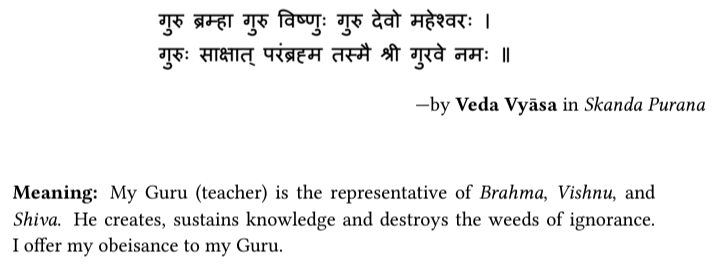
\includegraphics[width = 0.6\textwidth]{images/guru shlok.png}
    \label{fig:guru}
    \vspace{-0.5cm}
\end{figure}

This \textit{shlok} expresses the idea that \textit{guru} is revered as a divine entity, embodying the creative, preserving, and enlightening aspects of the divine. I would like to acknowledge and offer my sincere gratitude to the people who have played a pivotal role in shaping my academic journey at Dalhousie University.

\looseness=-1
First, I thank the Almighty, who granted me good health, intellectual capacity, and the fortitude to carry out my thesis. Then I want to express immense gratitude to my supervisor, Dr. Masud Rahman, for allowing me to join his research group and supporting me throughout my Master's studies. I thank him for motivating me and believing in me constantly, especially when I could not. His unwavering support, insightful feedback, and patience have been invaluable to me throughout my thesis work.

I would like to express my sincere gratitude to Dr.\ Vlado Keselj and Dr.\ Tushar Sharma for their insightful feedback and thorough evaluation of my work. Their critical analysis and insightful comments have raised the standard and rigor of my thesis, and I sincerely appreciate their time and expertise.

To my beloved parents, Samar Kumar Mukherjee and Madhumita Mukherjee, for their support and love in every capacity throughout my life. Their guidance, encouragement, and sacrifices have been instrumental in shaping the person I am today and achieving this significant milestone in my life.

I would also like to thank my brother Udayan Mukherjee and my sister Shaniqua Mukherjee for guiding me all the way. Thank you for taking me to places that I never thought I could visit, for the amazing food and for also being my friends. I am also thankful to Flo for making me happy through the simplest of ways and being my unofficial mental health support dog. 

I would like to acknowledge the irreplaceable support and affinity of my precious friends Nikita Rathi and Isaac Xu for their friendship, support, and shared experiences. In particular, I would like to thank Nikita for taking care of me when I was sick, teaching me how to cook and also making me food. I would like to thank Isaac, for being my support system through this journey, for cheering me up when I was sad, and for teaching me about transformers. I thank both of them for being my best friends, and I consider myself lucky to have them by my side.

To all of the members of the Intelligent Automation in Software EngineeRing (RAISE) Lab -- Sigma Jahan, Ohiduzzaman Shuvo, Parvez Mahbub, Asif Samir, Riasat Mahbub, Shihui Gao, Lareina Yang, Callum MacNeil and Mehil B Shah with whom I have had the opportunity to grow as a researcher. I would also like to express my gratitude to all the members of the Software Maintenance and Analytics Research Team (SMART) Lab --- Indranil Palit, Gautam Shetty, Mootez Saad, Saurabhsingh Rajput and Himesh Nandani. I appreciate their efforts in making our work in the labs enjoyable and for engaging in meaningful discussions. In particular, I thank Sigma, Parvez, Shuvo and Mehil for making me feel at home despite being away from home. Special thanks go to Indranil and Mehil for bringing laughter to the group, especially on gloomy days.

Furthermore, I would like to thank Dalhousie University and the Department of Computer Science for creating a stimulating learning environment and providing the necessary resources for my research. The outcome of this thesis has been greatly influenced by their drive for intellectual progress and their commitment to excellence. In particular, I would like to thank Dr. Michael McAllister and Megan Baker.

Lastly, I extend my heartfelt thanks to all those who have supported me in various ways throughout this research endeavour. Your encouragement, advice, and assistance have been invaluable, and I am deeply grateful for your presence in my life.

\end{acknowledgements}

\mainmatter


\chapter{Introduction}

\section{Motivation}

Software bugs are human-made mistakes in a software system that prevent it from working as expected~\cite{ieeestandardglossaryforse}. Existing studies have shown that software bugs cost the global economy billions of dollars every year~\cite{britton2013reversible, zou2018practitioners}. Hundreds of software bugs are submitted to bug-tracking systems like GitHub and JIRA as \textit{bug reports}~\cite{anvik2006should}. These bugs are then triaged, analyzed, and resolved by developers. Developers spend $\sim$50\% of their programming time finding and fixing bugs~\cite{britton2013reversible}. Thus, bug resolution has been one of the major challenges in software maintenance~\cite{zou2018practitioners}.  A recent study suggests that up to 78\% of 32,198 bug reports collected from four open-source projects (e.g., Eclipse, Mozilla, Firefox, GCC) have less than 100 words each, which might not be sufficient (a.k.a., short bug reports)~\cite{zhang2017bug}. These short bug reports required 121 days extra on average for their resolutions as opposed to the well-written bug reports~\cite{zhang2017bug}. That is, missing information in bug reports could lead to their delayed resolution~\cite{zhang2017bug}. According to a recent survey~\cite{zou2018practitioners}, 77\%  of 327 software practitioners (e.g., developers, testers, managers) from the major technology companies (e.g., Google, Meta, Amazon, Microsoft) consider missing information as a major problem and emphasize on complementing bug reports with useful information (e.g., steps to reproduce, environmental configuration)~\cite{zou2018practitioners}. Missing information has also been found to be a key factor behind the non-reproducibility of software bugs~\cite{rahman2020some}. Thus, missing information has been a major challenge and complementing the bug reports with relevant information would greatly benefit the developers in their bug resolution.\par
\begin{figure} [!htbp]
    \centering 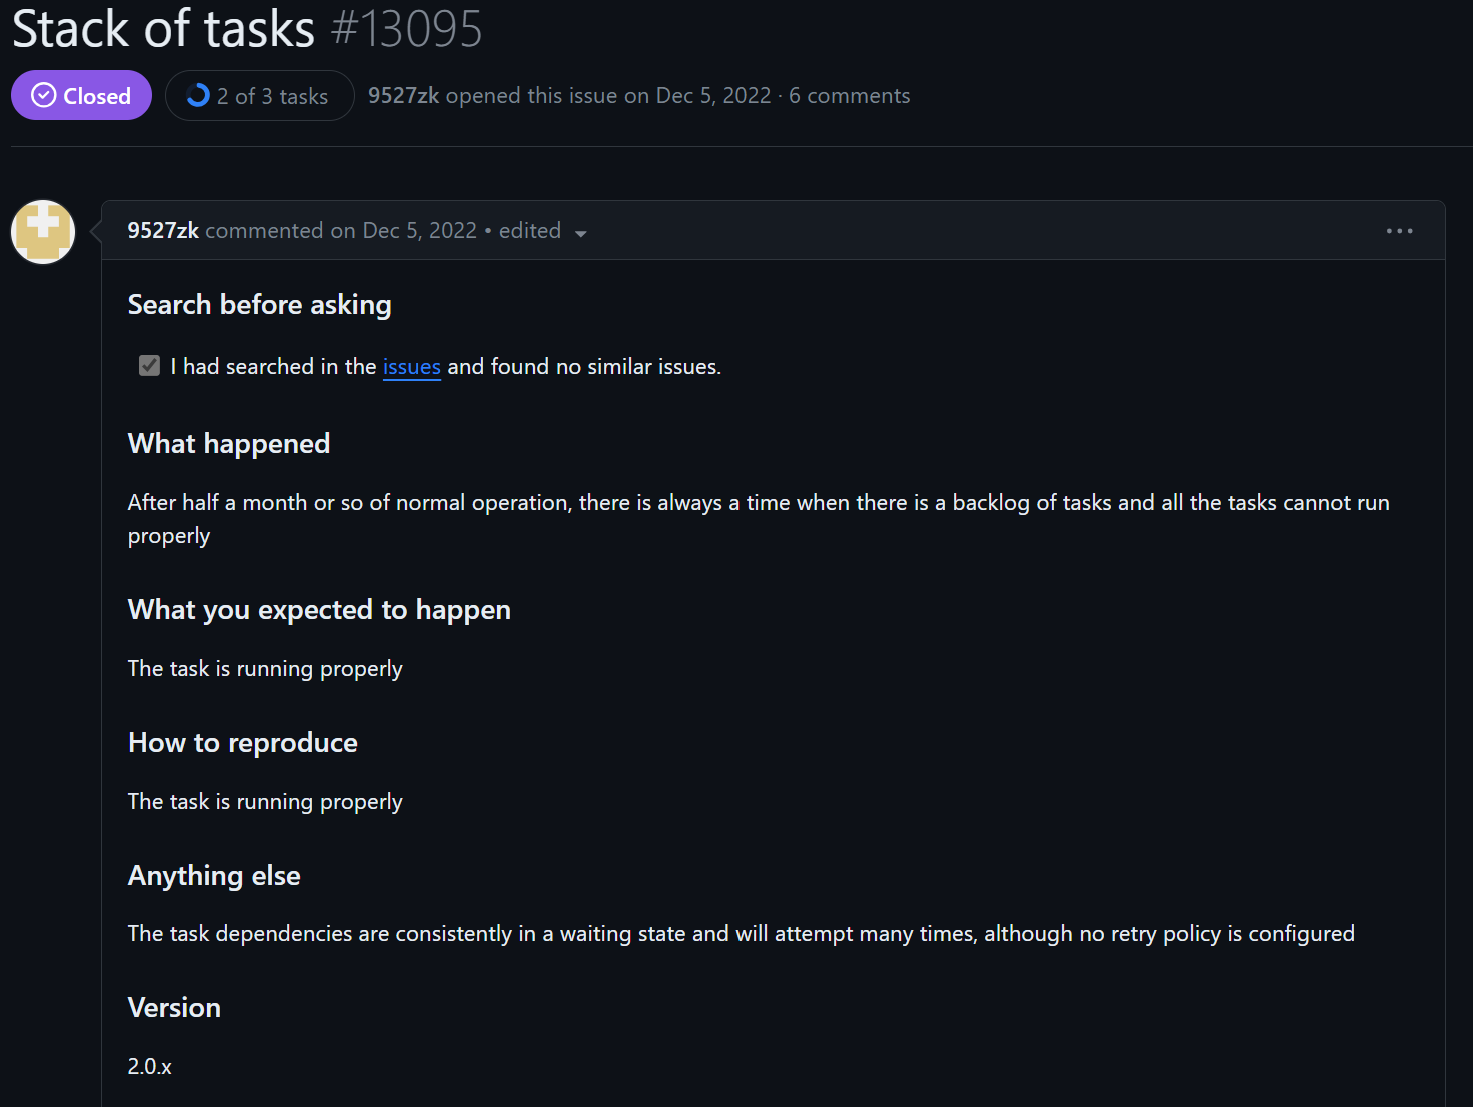
\includegraphics[width=0.8\textwidth]{images/intro_missing_info_eg.png} 
    \caption{An example bug report with missing information (ID \#13095)}
    \label{fig:missinginfo}
\end{figure}

Ideally, bug reports should contain all the information, such as system configuration, expected behaviour, observed behaviour, and reproducing steps that help a developer resolve a bug~\cite{chaparro2017detecting}. However, in practice, they often do not contain all the required information for reproducing or resolving a bug~\cite{chaparro2017detecting}. Let us consider the example bug report in Fig. \ref{fig:missinginfo}. It discusses a task backlog problem where the task dependencies are consistently in a waiting state. However the reporter does not provide any system configuration details, logs or steps to reproduce. As a result, the report was later marked as ``needs more information" and then closed. According to existing literature~\cite{chaparro2017detecting},  64.8\% of bug reports do not contain any expected behaviour of target software systems, and 48.6\% of them do not explicitly describe the steps to reproduce a bug. Many software projects on GitHub now require the bug reports to adhere to specific templates or standard guidelines~\cite{githubguidelines}. However, many bug reporters might fail to comply with them and might not be able to provide all the information during report submission~\cite {imran2021automatically}. Developers thus often pose \textit{follow-up} questions to bug reporters soliciting the missing information. Unfortunately, the bug reporters often find it challenging to answer the follow-up questions in a timely fashion, according to a recent developer survey ~\cite{rahman2020some}. Such a lack of responses could lead to non-reproducible or unresolved bugs~\cite{breu2010information}. However, there has been only a little research investigating the follow-up questions from bug reports or their answers.

\begin{figure}[!htpb]
  \centering
  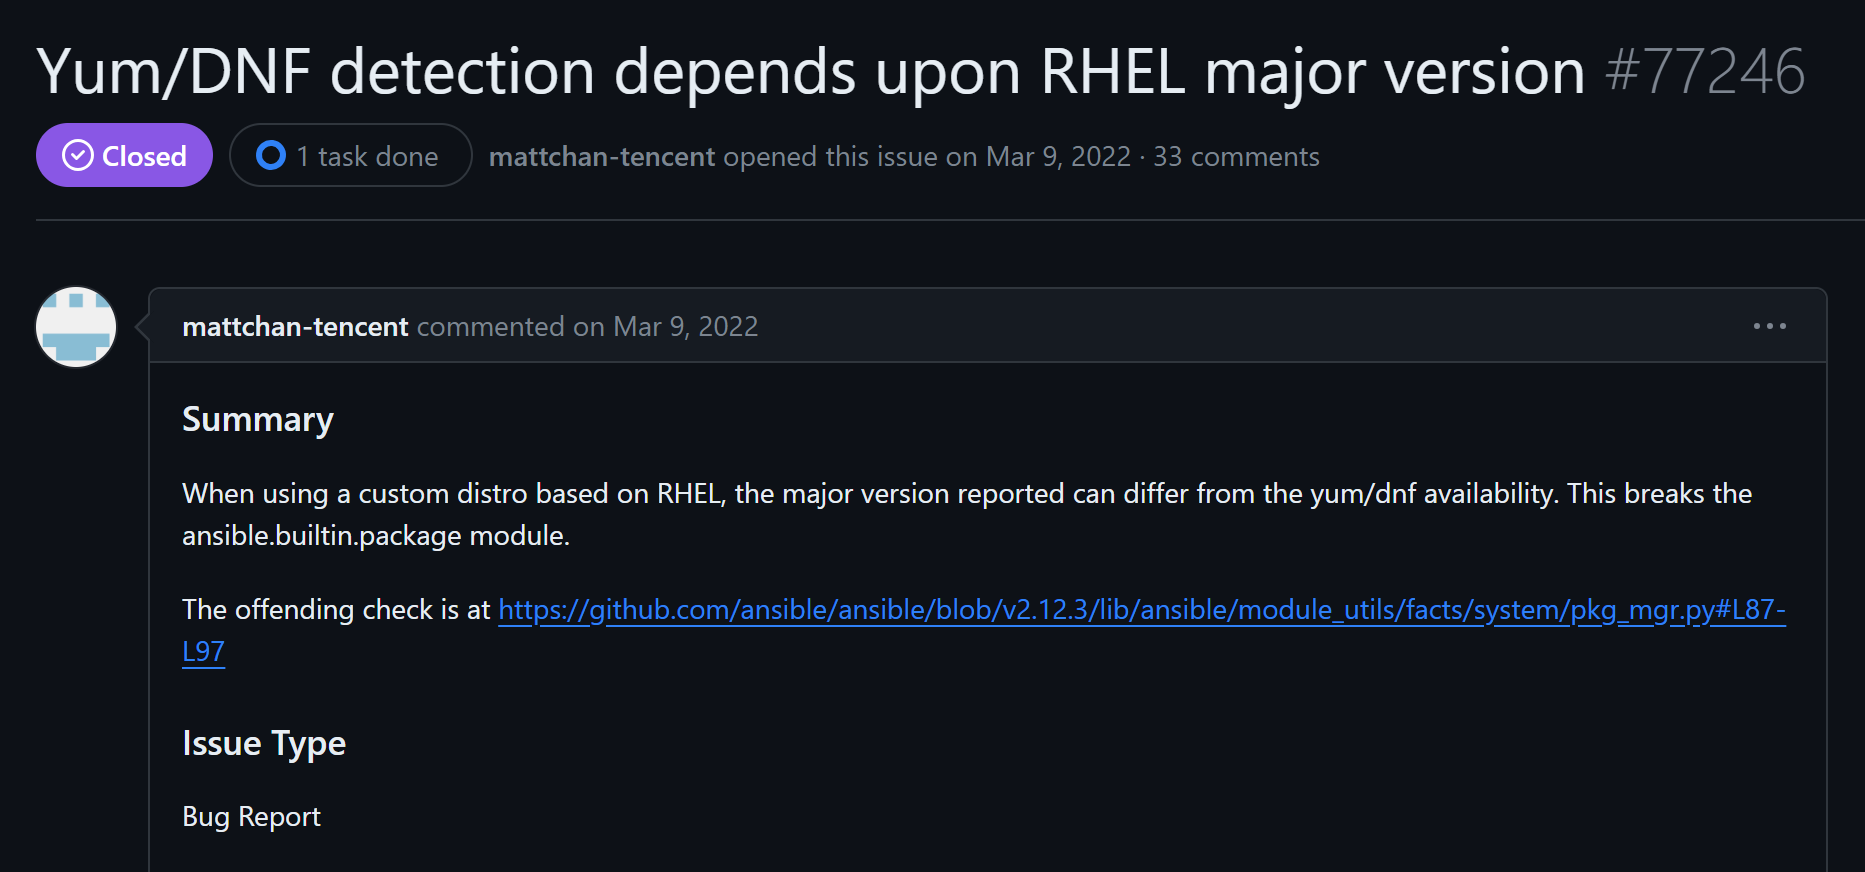
\includegraphics[width=0.8\textwidth]{images/not_readable_bug_report.png}
  \caption{ An example bug report (ID \#77246)}
  \label{Intro-fig:notreadbleBR}
\end{figure}

Answers to the follow-up questions provide more contextual information regarding a reported bug, which could help the developers resolve the bug. However, newcomers or novice developers to a project might need additional help to accurately understand or resolve a bug. In particular, complex contextual information and the incomplete or inaccurate content in bug reports could make bug understanding a challenging task~\cite{velly2013towards}. Let us consider the example bug report in Fig. \ref{Intro-fig:notreadbleBR}. The bug report uses several software-specific terms such as ``custom distro'', ``RHEL'' and ``yum/dnf". It discusses the ansible version mismatch between the custom distribution of Red Hat Enterprise Linux (RHEL) and the Yellowdog Updater Modified (yum)/dandified YUM (dnf) package management tool. To a newcomer, all these terminologies could be daunting and discouraging. However, decoding them is essential to understand and diagnose the reported bug. 
% This discrepancy poses a challenge, potentially causing a malfunction in the ansible.builtin.package module, which relies on accurate version information for proper execution. 
According to an existing study~\cite{guizani2021long}, even with prior experience, developers often struggle to acquire a comprehensive understanding of any application domain and understand the discussions from a bug report. Thus, a lack of explanation for the domain-specific terms or jargon could be a major issue towards bug understandability.

\section{Problem Statement}

Bug reports are a valuable resource for software maintenance and continuous evolution. Over the last few decades, there has been extensive research to support various bug report management tasks, including bug triage ~\cite{zhao2019unified}, ~\cite{bodden2017proceedings}, issue report classification ~\cite{thung2012automatic}, ~\cite{nayrolles2018towards}, duplicate bug report detection~\cite{nguyen2012duplicate, chaparro2019reformulating}, and bug localization ~\cite{zhang2019finelocator}, ~\cite{xiao2019improving}. However, the problem of missing information or domain-specific jargon in bug reports has not been comprehensively studied or addressed. Given the evidence above, adding complementary information to deficient bug reports could greatly benefit software practitioners in their work.\par

There have been existing studies that provide complementary information through Question Answering (QA) to support various software engineering tasks. Tian et al.~\cite{tian2017apibot} designed APIBot that can answer questions related to an API by analyzing relevant API documentation. Bansal et al.~\cite{bansal2021neural} designed a context-aware QA system to answer basic questions about subroutines. Lu et al.~\cite{lu2021beat} proposed a QA approach that can provide answers by executing structured queries generated from bug templates. However, there has been only a little research investigating the follow-up questions from bug reports or their answers. Breu et al.~\cite{breu2010information} first conducted a mix of quantitative and qualitative analysis on follow-up questions and found that 32.34\% of the questions were never responded to. They suggest that the questions in the bug reports were critical to the effective triaging, reproduction and resolution of a bug. Recently, Imran et al.~\cite{imran2021automatically} proposed a technique that recommends follow-up questions against a deficient bug report using structured information retrieval. Although both studies above deal with the follow-up questions from a bug report and are a source of inspiration, they do not answer the questions.\par

There have been existing studies to support newcomers or inexperienced developers who may struggle to comprehend software bug reports. An existing survey by Tan et al.~\cite{tan2020first} suggests that a clear description of a bug that does not rely on in-depth domain knowledge is necessary to help newcomers understand and resolve the bug. Recently, Correa et al.~\cite{correa2013samekana} suggest that the inclusion of web links (to external knowledge sources or artifacts) in the issue tracker discussion can benefit the developers. Zhang et al.~\cite{zhang2017bug} propose to supplement a bug report with a list of sorted sentences that are extracted from past, relevant bug reports. Dit et al.~\cite{dit2008improving} proposed a technique that recommends relevant comments so that the developers can make explicit connections between the recommended comments and existing ones. Such connections could help the developers better understand a bug report. While the above approaches offer complementary information to support bug understanding, they do not focus on the domain-specific terms or jargon, which warrants for further investigation.\par

% research problem without lit
Given the above discussions, missing information is one of the key factors that affect developers when comprehending software bug reports and could lead to delayed bug delayed reproduction and resolution. It affects bug reports in two different ways. First, bug reports often do not contain sufficient information for timely resolution. Developers thus pose follow-up questions asking the bug reporter for missing information. However, bug reporters or any user facing a similar bug may find it challenging to answer them due to a lack of domain-knowledge. Second, bug reports may contain domain-specific terms or jargon that may not be well understood by novice or newcomer developers. Traditional bug tracking systems do not provide any support to comprehend such domain-specific terms or jargon. To the best of our knowledge, existing literature might also not be sufficient to enhance the bug reports plagued by missing information. We thus perform two studies to complement such deficient bug reports with missing information using automated tools and technologies. \par

 
\section{Our Contribution}
In this thesis, we propose and evaluate two novel techniques that support developers in bug resolution by complementing a deficient bug report in two different ways.

In our first study, we propose a novel technique --- \textit{BugMentor} --- that can offer relevant answers to follow-up questions from bug reports by combining structured information retrieval and neural text generation. First, we capture textually relevant questions, answers, and bug reports against a follow-up question using structured information retrieval~\cite{saha2013improving}. Then we capture each item's embeddings using Word2Vec~\cite{efstathiou2018word} and re-rank them based on their semantic relevance to the question. Second, we generate meaningful answers to the follow-up question by leveraging the ranked items above as \textit{context} with a neural text-generation technique (e.g., CodeT5).

We evaluate answers from \textit{BugMentor} using four performance metrics ---  BLEU score~\cite{papineni2002bleu}, METEOR~\cite{banerjee2005meteor}, Semantic Similarity~\cite{haque2022semantic}, and WMD~\cite{huang2016supervised}. We achieve a BLEU score of 34.12 which indicates that our generated answers are \textit{understandable} to \textit{good} according to Google AutoML documentation~\cite{automldoc}. We also conduct an ablation study to justify our combination of structured information retrieval and neural text generation in BugMentor. We find that BugMentor can capture a rich context leveraging structured information retrieval and thus can generate meaningful answers. BugMentor also outperforms all three baselines --- Lucene~\cite{mccandless2010lucene}, CodeT5~\cite{wang2021codet5}, AnswerBot~\cite{xu2017answerbot} --- in all four metrics.  To further demonstrate its benefit, we conduct a developer study involving 10 participants. According to the participants, the answers from BugMentor were more accurate, more precise, more concise and more useful compared to the baseline answers.


In our second study, we propose -- \textit{BugEnricher} -- a novel technique that can enhance bug reports with meaningful explanations to their domain-specific terms or jargon using neural text generation. First, we collect thousands of domain-specific vocabulary and their explanations from three different sources -- StackOverflow, API documentation, and glossary. Second, we fine tune the T5 model~\cite{raffel2020exploring} on our collected vocabulary and explanations. Third, we use \acrshort{TF-IDF} to extract the infrequent domain-specific terms from each bug report. Finally, we generate natural language explanations to the domain-specific terms or jargon using our fine-tuned T5 model. \par

Our evaluation using three performance metrics shows that \textit{BugEnricher} can generate \textit{understandable} and \textit{good} explanations according to Google’s standard, and can outperform two existing baselines --- T5~\cite{raffel2020exploring} and AnswerBot~\cite{xu2017answerbot} --- from the literature. To further demonstrate the benefit of our explanations, we conduct a case study using the bug reports enriched with explanations. We evaluate the performances of an existing technique~\cite{yang2012duplication} for duplicate bug report detection that is impacted by the problem of textually dissimilarity~\cite{jahan2023towards}. We find that the enriched bug reports were able to improve the performances of the existing technique in detecting textually dissimilar duplicate bug reports.\par

Given the empirical evidence, our proposed techniques have the potential to significantly improve the bug report management and their resolution.

\section{Related Publications}
Several parts of this thesis are either submitted or ready to be submitted to different conferences.
We provide a list of papers here. In each of these papers, I am the primary author, and all the studies were conducted by me under the supervision of Dr. Masud Rahman. While I wrote these papers, the co-author took part in advising, editing, and reviewing the papers.
\begin{itemize}
    \item \emph{Usmi Mukherjee} and M. Masudur Rahman. \emph{Answering Follow-up Questions from Bug Reports Leveraging Structured Information Retrieval with Neural Text Generation}. In Proceedings of the 47th International Conference on Software Engineering (ICSE 2025), pp.13, Ottawa, Canada, April-May 2025.(Pre-submission)
\end{itemize}

\begin{itemize}
    \item \emph{Usmi Mukherjee} and M. Masudur Rahman. \emph{BugEnricher: Explaining Domain-specific Terms and Jargon from Bug Reports with Neural Machine Translation}. In Proceeding of the 40th IEEE International Conference on Software Maintenance and Evolution (ICSME 2024), pp. 12, Flagstaff, Arizona, October 2024 (Pre-submission).
\end{itemize}

\section{Outline of the Thesis}

The thesis contains five chapters in total.
To complement missing information in bug report effectively, we conduct two independent but interrelated studies, and this section outlines different chapters of the thesis.

\begin{itemize}
    \item Chapter 2 discusses several background concepts (e.g., embedding, transformers, neural language modeling) that are required to follow the rest of the thesis.

    \item Chapter 3 discusses our first study that proposes \textit{BugMentor}, a novel approach that combines neural text generation (e.g., CodeT5) and structured information retrieval to generate appropriate answers to the follow-up questions.

    \sloppy
    \item Chapter 4 discusses our second study that proposes \emph{BugEnricher}, a novel transformer-based generative model that generates natural language explanations for software-specific terms in Bug Reports.

    \item Chapter 5 concludes the thesis with a list of directions for future works.
\end{itemize}
\chapter{Background}

In this chapter, we introduce the required terminologies and concepts to follow the remaining of the thesis. 
Section \ref{background:LM} discusses \acrfull{nlm}, a deep learning based approach to learn the probability distribution of a textual corpus. Section \ref{background:NMT} discusses \acrfull{nmt}, a deep neural network based approach for automated translation. Section \ref{background:StructuredIR} discusses structured information retrieval for question answering. Section \ref{background:WordEmbedding} describes embedding, the process of converting high dimensional vector data into low dimensional semantic representation. 
Section \ref{domaintermsdef} discusses the definition of domain-specific terms or jargon that are present in software bug reports.
Section \ref{background:TF-IDF} discusses TF-IDF, a statistical measure for determining the importance of a term in a document.\par

\section {Neural Language Modelling}\label{background:LM}

A language model is a probabilistic model for natural language texts. It generates the probability of occurrence of a word or a phrase within a given text corpus. Such probability distributions could be useful in various tasks. For example, in a text generation task, a language model predicts the next word $w_L$  on the basis of all preceding words and their probability of co-occurrence~\cite{hu2018deep,mahbub2023comprehending}.\par

\begin{equation}
    w_L = \arg\max_{w_v \in V} P(w_v | w_{L-1} w_{L-2} ... w_1)
\end{equation}

where $w_L$ is the next predicted word, $V$ is the vocabulary, and $w_{L-1}, w_{L-2}, ..., w_1$ are the previously predicted words.\par

Neural language models use neural networks to capture the complex patterns and dependencies of natural language and leverage them to compute the probabilities of the next word. In particular, they attempt to predict the next word while estimating the numerical representation of the words and texts (a.k.a., embeddings)~\cite{zhang2021natural}. Our first study -- BugMentor -- uses neural language modelling to generate answers to follow-up questions. Our second study -- BugEnricher -- uses neural language modelling to generate explanations for domain-specific jargon.\par

\section{Neural Machine Translation}\label{background:NMT}

\acrfull{nmt} is an automated translation technique based on deep neural networks ~\cite{wu2016google}. NMT has made significant progress, capturing the attention of both researchers and practitioners. It supports various software engineering tasks such as automatic program repair~\cite{lutellier2020coconut,jiang2021cure}, commit message generation~\cite{jiang2019boosting}, and code summarization~\cite{leclair2019neural}. An \acrshort{nmt} model consists of two main components: an encoder and a decoder. The encoder accepts a sequence as input and uses Neural Language Modeling to construct a numerical representation of the input called the context vector. This context vector is then fed into the decoder, which, based on this vector, sequentially generates the target sequence, one token at a time. We use Transformer~\cite{raffel2020exploring,vaswani2017attention} based state of the art \acrshort{nmt} models -- CodeT5~\cite{wang2021codet5} and T5~\cite{raffel2020exploring} as a part of our studies. In our first study -- BugMentor, we use \acrshort{nmt} for generating answers to the follow-up questions from bug reports. In our second study -- BugEnricher, we use \acrshort{nmt} for generating explanations for domain-specific terms or jargon from bug reports.\par


\section{Structured Information Retrieval} \label{background:StructuredIR}

\acrfull{ir} is a popular method that facilitates access to vast repositories of information (e.g., World Wide Web).
In traditional IR, there are two major components: query and corpus. The query consists of a few keywords, whereas the corpus represents a collection of searchable documents. These queries and corpus are preprocessed using standard natural language preprocessing techniques such as text normalization, stopword removal and lemmatization. The query corpus is also indexed by collecting various statistics such as term frequency (TF, the number of times a term occurs in a given document) and document frequency (DF, the number of documents in which the term appears)~\cite{saha2013improving}. These terms and document statistics are then used in algorithms such as TF-IDF and BM25. Traditional IR, however, does not take into account the underlying structure of the query and the corpus. Structured IR is found to be more effective in retrieving. It has the potential to reduce noise and spurious matching due to the structured nature of the search. For example, in our first study, BugMentor uses three main components of the bug reports -- title, description, and follow-up questions -- that are used to match with the corpus bug reports. Structured IR divides both query and document into granular abstractions and calculates the lexical similarity between them~\cite{saha2013improving}.
   

\section{Word Embedding} \label{background:WordEmbedding}

Word embedding is a vector representation of words in a \acrfull{vsm}. It encodes the meaning of the word in such a way that semantically similar words are closer to each other within the vector space~\cite{moser2008comparative}. An embedding function $E: \mathcal{X} \rightarrow \mathbb{R}^d$ takes an input $X$ in the domain $\mathcal{X}$ and generates its vector representation in a $d$-dimensional vector space~\cite{cambronero2019deep}. Each word or phrase is mapped to a vector of real numbers that represent the meaning of the input~\cite{mahbub2022explaining}. 
Word embedding can overcome issues faced by traditional \acrshort{vsm}, such as the sparse representation problem of one-hot encoding or the vocabulary mismatch issue of \acrshort{TF-IDF} and BM25. Several techniques employ neural networks to learn richer word representations, such as Word2Vec~\cite{mikolov2013distributed} and GloVe~\cite{pennington2014glove}. We use Word2Vec embeddings to determine semantic relevance between bug reports in our first study, BugMentor.

\section{Domain-specific Terms or Jargon}\label{domaintermsdef}
Domain-specific terms or jargon are specialized vocabularies for a particular application domain such as programming language, library or software. They may have specific meanings or interpretations unique to that domain. They can be categorized based on their type, application domain (e.g., Android, Firefox), domain concepts (e.g.,semantic labels/classes) ~\cite{kim2011classifying, fowler2010domain}. The explanations or meanings for domain-specific terms can be found in their corresponding documentation and glossary. In our second study, BugEnricher, we explain the domain-specific terms or jargon from several domains including two programming languages - Java and Python.

\section{TF-IDF}\label{background:TF-IDF}
Term Frequency - Inverse Document Frequency (TF-IDF) is a statistical measure of the importance of a term within a document. Each word in the document can have a \acrshort{TF-IDF} score. First, the Term Frequency (TF) is computed using the occurrence of each term within a document and can be normalized using the total number of terms in the document as follows.
\begin{equation}
\text{tf}(t, d) = \frac{\text{number of times term } t \text{ appears in document } d}{\text{total number of terms in document } d}
\end{equation}
Second, the Document Frequency (DF) refers to the number of documents containing the term. Words unique to a small percentage of documents (e.g., technical jargon terms) receive higher importance than the common words across all documents (e.g., a, the, and). Inverse Document Frequency (IDF) measures the rarity or uniqueness of a term across the entire collection of documents by inverting the DF as follows.
\begin{equation}
{ DF(t) = occurrence\ of\ term\ t\ in\ N\ documents \\}
\end{equation}
\begin{equation}
    IDF(t) = log(N/(DF(t) + 1))
\end{equation}
Finally, the TF-IDF score is the product of the TF and IDF scores. The greater the TF-IDF score, the more significant the term in that document~\cite{tfidf}.
\begin{equation}
\text{tf-idf}(t, d) = \text{tf}(t, d) \times \text{idf}(t)
\end{equation}
We compute the TF-IDF score to determine the less frequent but important domain-specific terms or jargon from a bug report in our second study, BugEnricher.

\section{Summary}
In this chapter, we introduce different terminologies and background concepts to help one follow the remainder of the thesis. We discuss Neural Language Modelling in Section~\ref{background:LM}, deep learning based approach to learn the probability distribution of a textual corpus; Neural Machine Translation in Section~\ref{background:NMT}, a deep learning approach for automated translation; Structured Information Retrieval in Section \ref{background:StructuredIR} for effective retrieval of documents for a given query; Word Embeddings in Section~\ref{background:WordEmbedding} for vector representation of text; Section~\ref{domaintermsdef} defines domain-specific terms or jargon and TF-IDF in Section~\ref{background:TF-IDF} for determining important keywords in a document with respect to a collection of documents.
\chapter{BugMentor: Answering Follow-up Questions from Bug Reports Leveraging Structured Information Retrieval with Neural Text Generation}\label{chapter:BugMentor}


% \begin{abstract}
\looseness=-1
Software bug reports often lack crucial information (e.g., steps to reproduce), which makes bug resolution challenging. Developers thus ask follow-up questions to capture additional information. However, according to existing evidence, bug reporters often face difficulties answering them, which leads to the premature closing of bug reports without any resolution. Recent studies suggest follow-up questions to support the developers, but answering the follow-up questions still remains a major challenge. In this chapter, we propose BugMentor, a novel approach that combines neural text generation (e.g., CodeT5) and structured information retrieval to generate appropriate answers to the follow-up questions. 

The rest of this chapter is organized as follows. Section~\ref{Chap1:Intro} introduces our study and discusses the novelty of our work. Section~\ref{sec:motivating-example} discusses a motivating example to demonstrate the effectiveness of BugMentor. Section~\ref{Chap1:BugMentor} discusses our proposed technique. Section~\ref{Chap1:Experiment} presents our experimental design, datasets, and evaluation metrics. Section~\ref{Chap1:Evaluation} discusses the evaluation results of BugMentor. Section~\ref{Chap1:RelatedWork} discusses relevant works to our study. Section~\ref{Chap1:Threats} discusses the threats to the validity of our study. Finally, Section~\ref{Chap1:Summary} summarizes this study.

\section{Introduction} \label{Chap1:Intro}

\looseness=-1
Software bugs are human-made errors in a software system that prevent the software from working as expected~\cite{ieeestandardglossaryforse}. Studies have shown that software bugs cost the global economy billions of dollars every year~\cite{britton2013reversible, zou2018practitioners}. Developers also spend $\sim$50\% of their programming time finding and fixing bugs~\cite{britton2013reversible}. Thus, bug resolution has been one of the major challenges in software maintenance~\cite{zou2018practitioners}. Hundreds of software bugs are submitted to bug-tracking systems like GitHub and JIRA as \textit{bug reports} ~\cite{anvik2006should}. These bugs are then triaged, analyzed, and resolved by developers.\par



\looseness=-1
Ideally, bug reports should contain all the information, such as system configuration, expected behaviour, observed behaviour, and reproducing steps that help a developer resolve a bug~\cite{chaparro2017detecting}. However, in practice, they often do not contain all the required information for reproducing or resolving the bug~\cite{chaparro2017detecting}. According to existing literature~\cite{chaparro2017detecting},  64.8\% of bug reports do not contain any expected behaviour of target software systems, and 48.6\% of them do not explicitly describe the steps to reproduce a bug. Missing information like this has been found to be a key factor behind the non-reproducibility of software bugs~\cite{rahman2020some}. In a survey conducted by Zou et al.~\cite{zou2018practitioners}, 77\% of 327 professional developers from the major technology companies (e.g., Google, Meta, Amazon, Microsoft) consider missing information as a major problem and emphasize on complementing bug reports with useful information (e.g., steps to reproduce, environmental configuration)~\cite{zou2018practitioners}. In short, missing information has been a key challenge toward cost-effective bug resolution. \par



\looseness=-1
Many software projects on GitHub now require bug reports to adhere to specific templates or standard guidelines~\cite{githubguidelines}. Unfortunately, many bug reporters might fail to comply with them and might not be able to provide all the information during report submission~\cite {imran2021automatically}. Developers thus often pose \textit{follow-up} questions to bug reporters soliciting the missing information. Unfortunately, the bug reporters often find it challenging to answer the follow-up questions in a timely fashion, according to a recent developer survey ~\cite{rahman2020some}. For instance, Fig.~\ref{fig:motivating_example} shows how a bug report was closed prematurely without any resolution due to a lack of responses to the follow-up question posed by the developer.\par



\looseness=-1
Over the last few decades, there has been extensive research to support various bug report management tasks, including bug triage ~\cite{zhao2019unified}, ~\cite{bodden2017proceedings}, issue report classification ~\cite{thung2012automatic}, ~\cite{nayrolles2018towards}, duplicate bug report detection~\cite{nguyen2012duplicate, chaparro2019reformulating}, and bug localization ~\cite{zhang2019finelocator}, ~\cite{xiao2019improving}. However, there has been only a little research investigating the follow-up questions from bug reports or their answers. Breu et al.~\cite{breu2010information} first performed both quantitative and qualitative analyses on follow-up questions and found that 32.34\% of the questions were never responded to. According to them, these unanswered questions in the bug reports were critical to the effective triaging, reproduction and debugging of a bug. Recently, Imran et al.~\cite{imran2021automatically} proposed a technique that recommends follow-up questions against a deficient bug report using information retrieval. While both studies above deal with the follow-up questions of a bug report, they do not answer them.\par



\looseness=-1
Automated Question Answering (QA) has been an active research topic for decades in Information Retrieval (IR) and Natural Language Processing (NLP) communities~\cite{ravichandran2002learning,brill2002analysis,waltz1978english, iyyer2014neural,asaduzzaman2013answering, tian2017apibot, lu2021beat, bansal2021neural, xu2017answerbot, abdellatif2020msrbot}. There also have been several works in the context of software engineering. Tian et al.~\cite{tian2017apibot} designed APIBot that can answer questions related to an API by analyzing relevant API documentation. Bansal et al.~\cite{bansal2021neural} designed a context-aware QA system to answer basic questions about subroutines. Lu et al.~\cite{lu2021beat} proposed a QA approach that can provide answers by executing structured queries generated from bug templates. However, their approach might fail when a bug report does not contain the requested information. Xu et al.~\cite{xu2017answerbot} designed AnswerBot that can synthesize answers for a non-factoid technical question from StackOverflow Q\&A website. While the above approaches are a source of inspiration, they do not answer the follow-up questions posed by developers against the bug reports.\par




\looseness=-1
In this chapter, we propose a novel technique --- \textit{BugMentor} --- that can offer relevant answers to follow-up questions from bug reports by combining structured information retrieval and neural text generation. First, we capture textually relevant questions, answers, and bug reports against a follow-up question using structured information retrieval ~\cite{saha2013improving}. Then we capture each item's embeddings using Word2Vec~\cite{efstathiou2018word} and re-rank them based on their semantic relevance to the question. Second, we generate meaningful answers to the follow-up question by leveraging the ranked items above as \textit{context} with a neural text-generation technique (e.g., CodeT5) ~\cite{yu2022code}.\par



\looseness=-1
We select the top 20 popular projects from GitHub that use four programming languages and collect 30,869 bug reports from them for our experiments. We evaluate our technique using four popular metrics for text generation, namely BLEU score~\cite{papineni2002bleu}, METEOR~\cite{banerjee2005meteor}, Semantic Similarity~\cite{haque2022semantic}, and WMD~\cite{huang2016supervised}. We achieve a BLEU score of 34.12 which indicates that our generated answers are \textit{understandable to good} according to Google AutoML documentation~\cite{automldoc}. We also conduct an ablation study to justify our combination of structured information retrieval and neural text generation in BugMentor. We find that BugMentor can leverage the rich context captured through structured information retrieval and thus can generate meaningful answers. BugMentor also outperforms all three baselines --- Lucene~\cite{mccandless2010lucene}, CodeT5~\cite{wang2021codet5}, AnswerBot~\cite{xu2017answerbot} in all four metrics.  To further demonstrate its benefit, we conduct a developer study involving 10 participants. According to the participants, the answers from BugMentor were more accurate, precise, concise and useful compared to the baseline answers.\par



\looseness=-1
To summarize, we make three contributions in this work:
\begin{itemize}
\item[(a)] A novel technique --- BugMentor --- that can generate relevant answers to follow-up questions from bug reports by combining structured information retrieval and neural text generation (e.g., CodeT5).
\item[(b)] A comprehensive evaluation and validation of BugMentor using both popular performance metrics (e.g., BLEU score, METEOR score, WMD, Semantic Similarity) and a developer study involving 10 participants.
\item[(c)] A replication package~\cite{bugmentorreplicationpackage} that includes our working prototype, experimental dataset, and other configuration details for the replication or third-party reuse.
\end{itemize}



\section{Motivating Example} \label{sec:motivating-example}



\looseness=-1
To demonstrate the potential benefit of our work, let us consider the example bug report in Fig.~\ref{fig:motivating_example}. It has been taken from the \emph{tensorflow} repository which is maintained by the organization \emph{tensorflow} on GitHub~\cite{MotivatingExampleTensorflow}. The bug report (Step (a), Fig~\ref{fig:motivating_example}) discusses a memory allocation issue and provides minimal steps to reproduce the issue. However, it does not follow the standard issue template provided by GitHub~\cite{issueTemplate_Github} and lacks sufficient information about the system configuration. Subsequently, the developer (\textit{@mohantym}) requests the missing information as a follow-up question inquiring whether 
%such as system details and if 
they experienced the same issue on \textit{nightly} version of the software (Step (b), Fig.~\ref{fig:motivating_example}). However, neither the bug reporter (\textit{@DanielZanchi}) nor anyone else provided an answer to the follow-up question. As a result, the bug report was initially marked as stale (Step (c), Fig.~\ref{fig:motivating_example}) and later closed due to a lack of response (Step (d), Fig.~\ref{fig:motivating_example}).\par

\begin{figure}[!htpb]
  \centering
  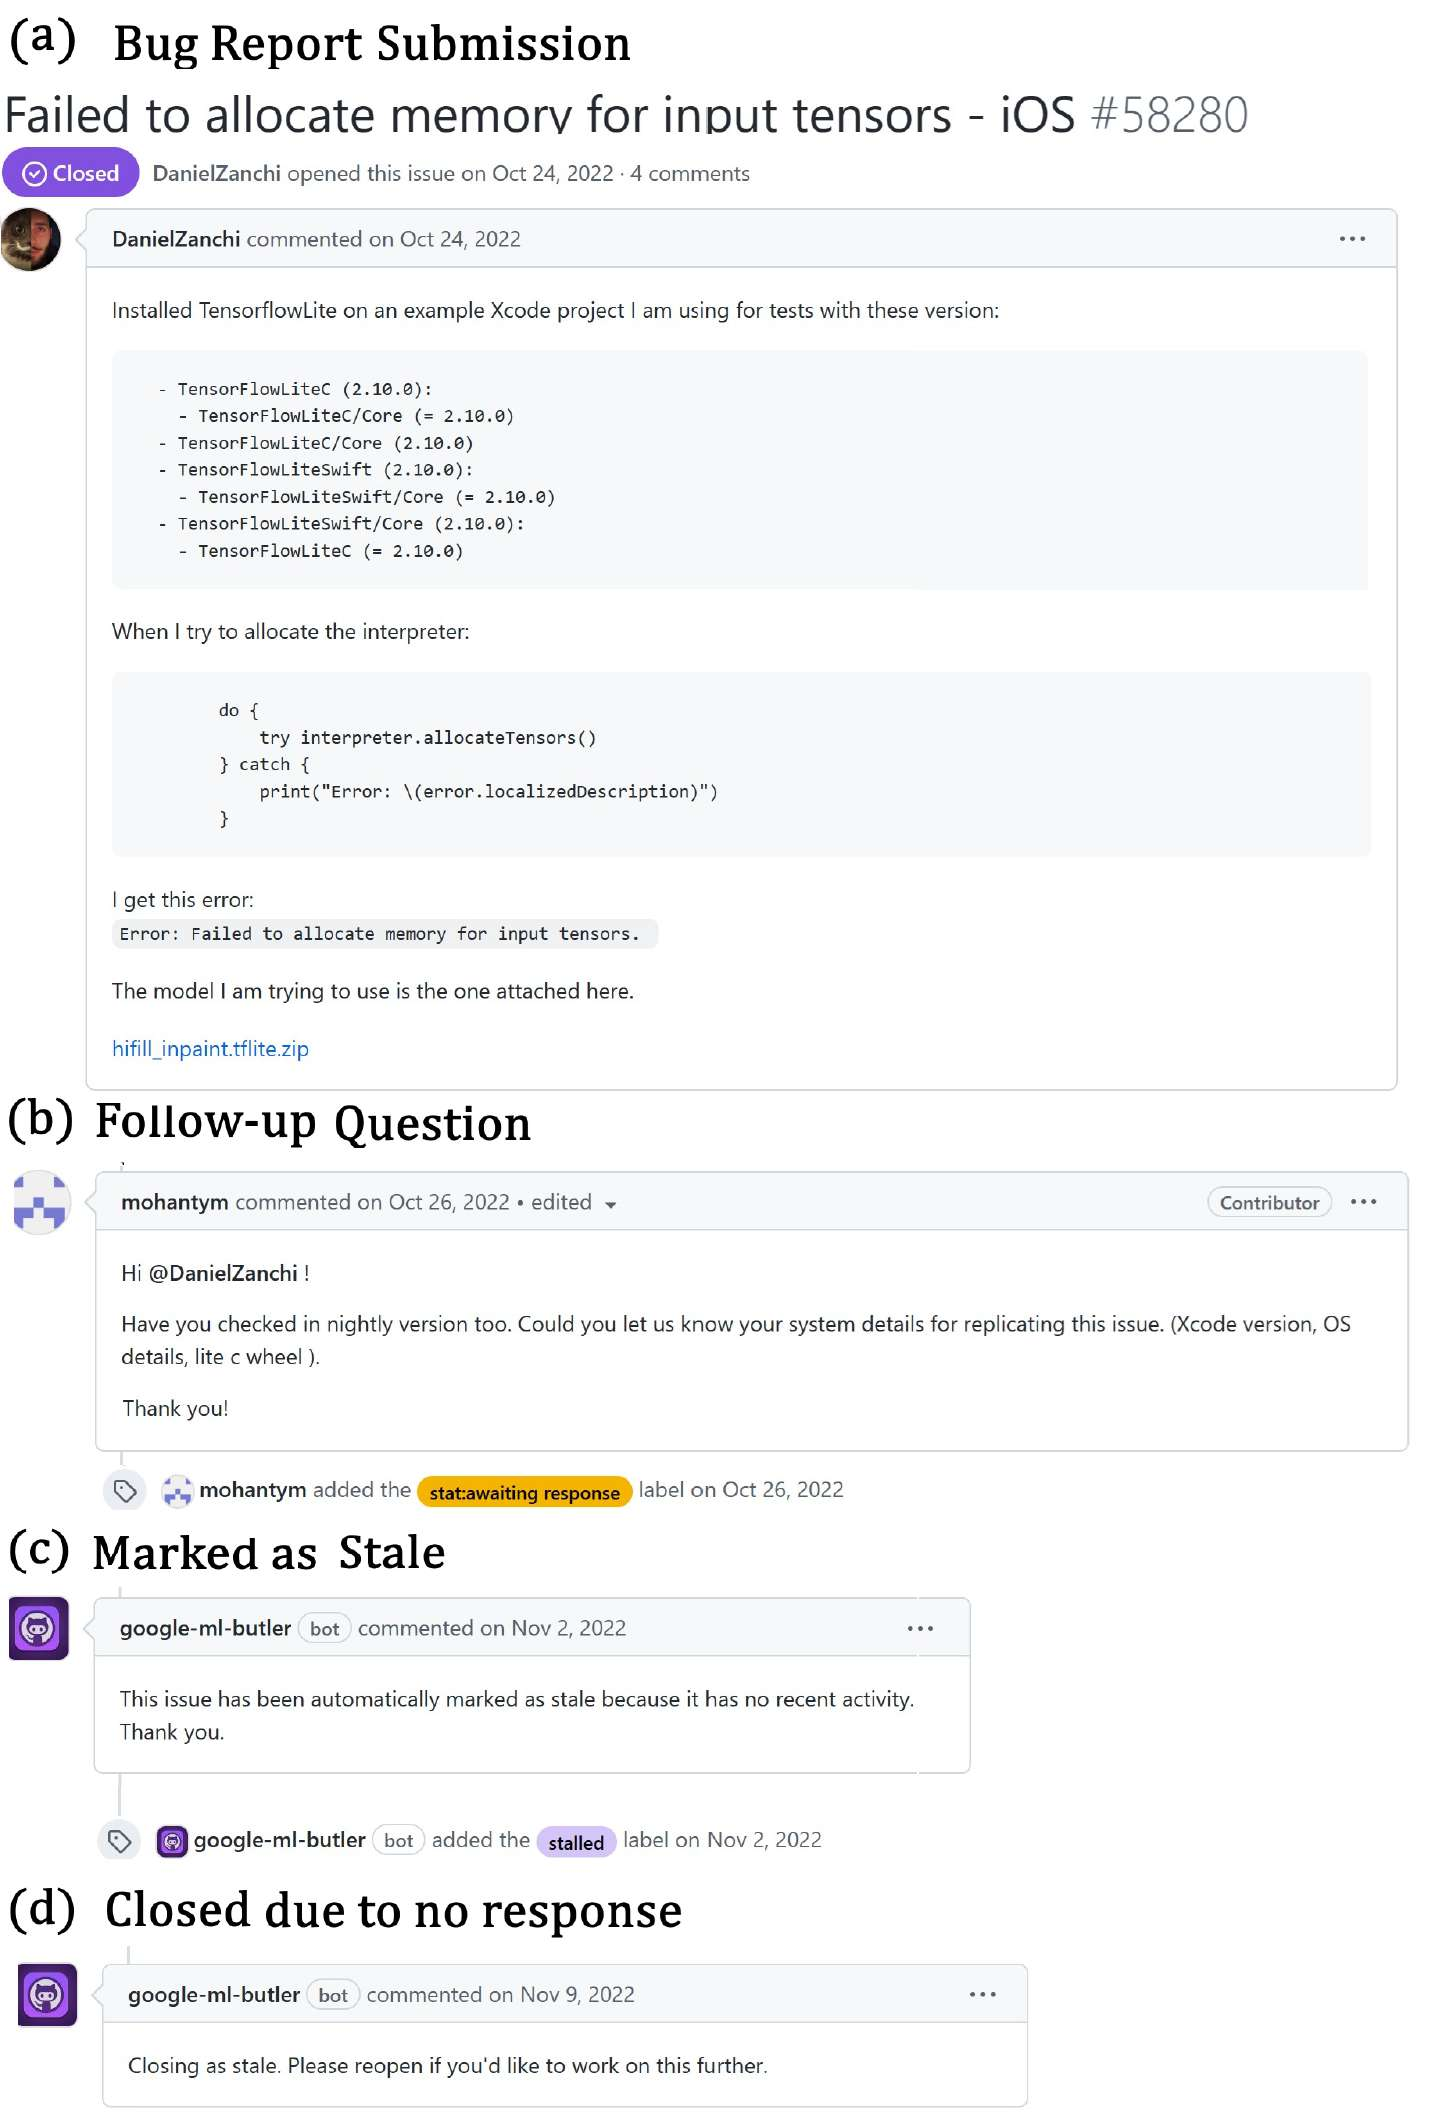
\includegraphics[ width=\textwidth, height=8.5in]{images/motivating_example_optimized.pdf}
  \caption{An example of a bug report (ID \#58280) being closed due to a lack of response to the follow-up question}
  \label{fig:motivating_example}
\end{figure}


\looseness=-1
As shown in Fig~\ref{fig:motivating_example}, without proper support in gathering missing information, software bugs either take longer to be resolved or remain unresolved and are ultimately closed. Several bugs, such as memory allocation bugs, are considered to be severe~\cite{li2006bugseverity} that significantly impact software quality. Our work --- BugMentor --- delivers meaningful answers to the follow-up questions, as shown in the answer for issue \#58280. \par

\begin{frshaded}
    % \vspace{-0.3cm}
    \begin{center}
        \textbf{Answer for issue \#58280 }
        % \label{bumentor-ans}
    \end{center}
        \noindent
        \textbf{Question:} Have you checked in nightly version too? Could you let us know your system details for replicating this issue (Xcode Version, OS details, lite c wheel)?\\
        \textbf{Generated Answer: }Adding two flags to Xcode's `Other Linker Flags' settings and modify the Podfile to use the nightly TensorFlow build, specifically `TensorFlowLiteSwift' and `TensorFlowLiteSelectTfOps'.
\end{frshaded}

\looseness=-1
We see that BugMentor was able to capture the context of the discussed problem above and provide useful suggestions. According to the bug report (Fig.~\ref{fig:motivating_example}), integrating the TensorFlow library into an Xcode project resulted in a memory allocation bug. BugMentor suggests modifying the \textit{``Other Linker Flags"} from Xcode to link the IDE to various versions of the TensorFlow library, such as \textit{TensorFlowLiteSwift} or \textit{TensorFlowLiteSelectTfOps}. It should be noted that these library versions were carefully extracted by our technique from the problem context in the bug report. Furthermore, BugMentor was able to deliver complementary information (e.g., \textit{Other Linker Flags}) that could be useful in resolving the library integration problem. The effectiveness of such an idea was further confirmed by a discussion on StackOverflow Q\&A site~\cite{linkerflags}.
% \vspace{-0.1cm}

% \vspace{-0.4cm}


\section{BugMentor: Proposed Technique} \label{Chap1:BugMentor}


\begin{figure}[htbp]
  \centering
  \rotatebox{270}{%
    \begin{minipage}{\textheight}
      \centering
      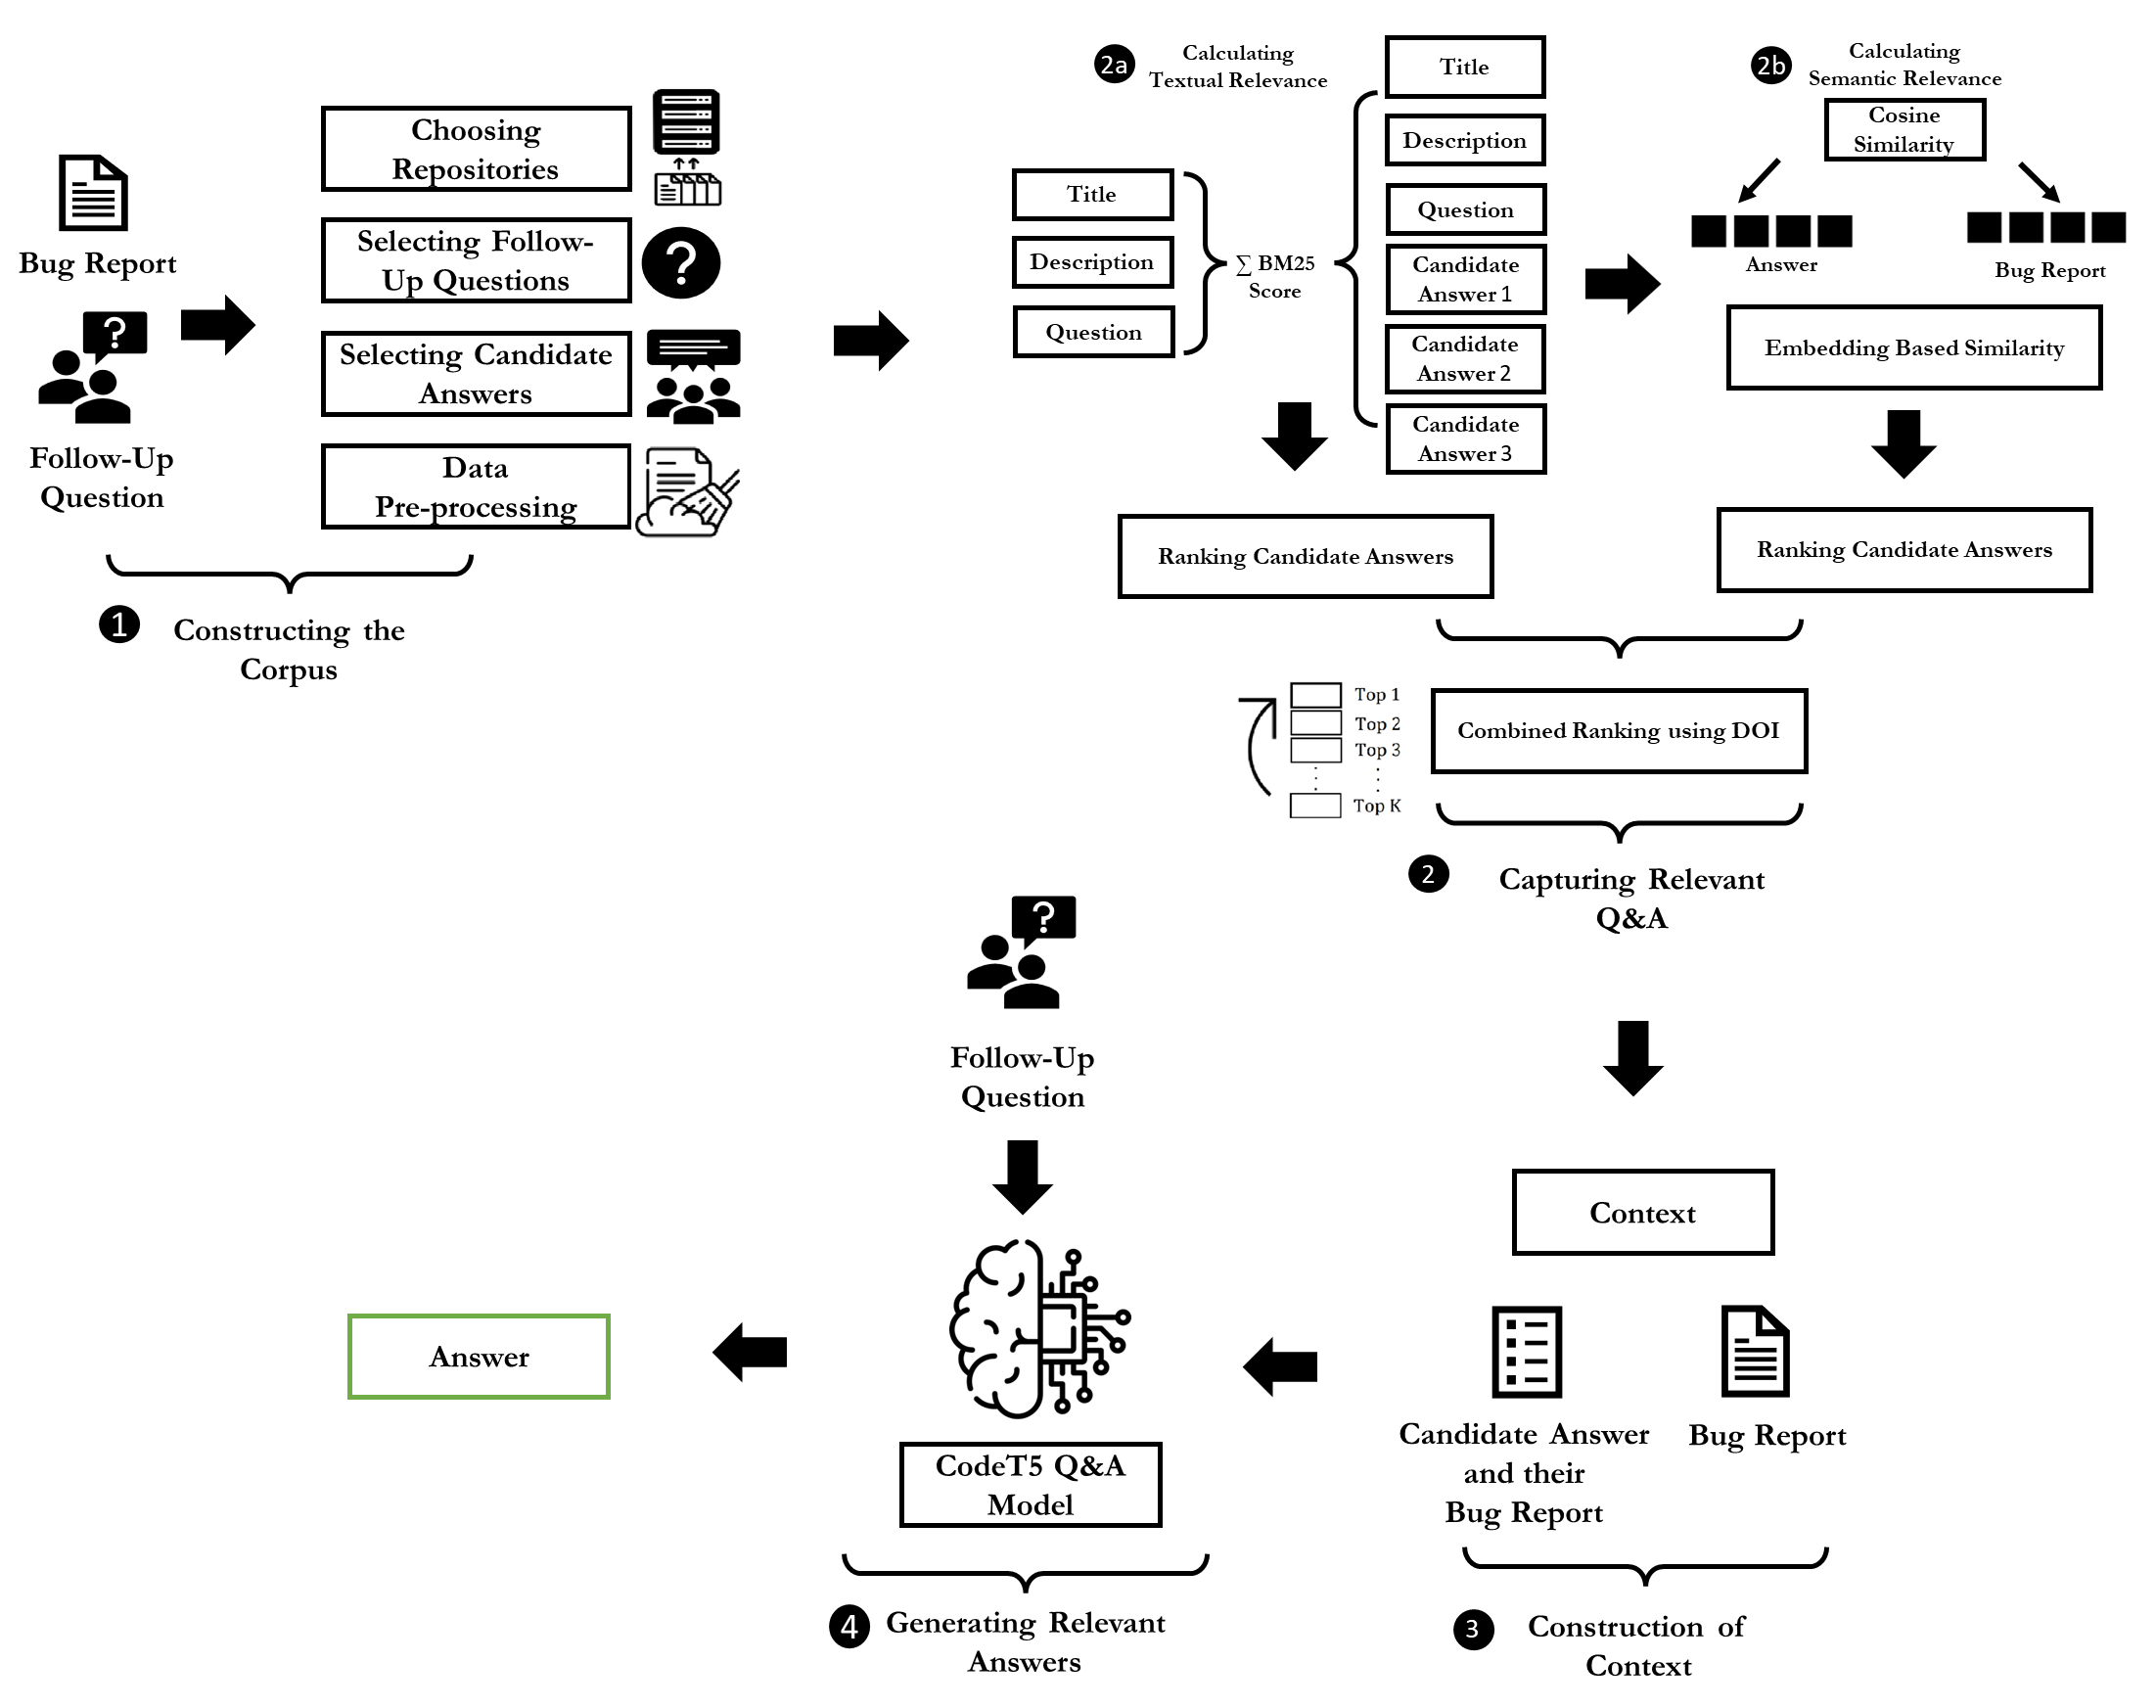
\includegraphics[width=0.9\textwidth, height=\textwidth,keepaspectratio]{images/BugMentorSchematic3.png}
      \caption{Schematic diagram of BugMentor}
      \label{fig:algo}
    \end{minipage}%
  }
\end{figure}

\looseness=-1
Fig.~\ref{fig:algo} shows the schematic diagram of our proposed technique --- BugMentor. As the input, it accepts a bug report of interest, its follow-up question, and a corpus of past bug reports with their follow-up questions and corresponding answers. As the output, our technique generates a relevant answer to the follow-up question. We discuss different steps of our technique in detail in the following sections.\par

\subsection{Constructing the Corpus}
\label{sec:corpus-construction}
\looseness=-1
We construct our corpus using past bug reports and their discussion history from 20 real-world open-source software systems on GitHub (Step 1, Fig~\ref{fig:algo}).\par


\subsubsection{\textit{Choosing the Repositories for the Corpus}}
\label{sec:proposedtechnique-repo}
To construct our corpus, we collect high-quality repositories using a semi-automated approach. We follow the approach of Imran et al. ~\cite{imran2021automatically} and choose GitHub~\cite{github} as a data source. GitHub~\cite{github} is a popular open-source platform that supports various software maintenance practices, including bug report management. We select the repositories and collect the bug reports as follows.\par

First, we select the most starred active repositories containing a minimum of 500 issues (reported as of May 2023) using GitHub's advanced search~\cite{GitHubAdvancedSearch}. We then categorize the repositories into four subsets based on their programming languages --- Python, Java, Javascript and C++ --- where each programming language had five repositories.\par

\subsubsection{\textit{Choosing the Bug Reports for the Corpus}}
\looseness=-1
From each repository, we then select the issues that were closed within the last five years. We select the issues that are labelled as ``bug", ``crash", or ``defect" to ensure that they are discussing software bugs or defects. We also select the bug reports labelled as ``needs more info" and ``stale" that were closed due to a lack of activity. We use GitHub's REST API~\cite{githubdocumentation} to collect the bug reports and their discussion history. Each of our collected bug reports consists of several fields, namely issue ID, title, bug description, bug reporter, label, creation time, and resolution time. \par

\subsubsection{\textit{Selecting Follow-up Questions}}
\label{sec:proposedtechnique-followq}
To select follow-up questions from each bug report, we first collect their issue comments using a GitHub API client~\cite{koshukeGitHubLibrary}. From each comment, we capture four different fields, namely --- comment ID, author of the comment, comment, and comment time. Following the strategy of Imran et al. ~\cite{imran2021automatically}, we collect the comments that begin with an interrogative word and end with a question mark. We use NLTK's Classifier~\cite{nltkclassifydocumentation} to identify these comments, as was applied previously~\cite{yuan2012enhancing}. We also consider comments that requested additional information using words such as ‘please’ or `can you' as valid comments. Then we select the first valid, interrogative comment that is not written by the author as our follow-up question from each bug report. We manually check up to 30 comments from each bug report to identify our follow-up questions. \par

\subsubsection{\textit{Selecting Candidate Answers}}
\label{sec:proposedtechnique-candidateans}
The next step in our corpus construction is to select candidate answers against the follow-up questions above. 
We apply three criteria to the selection of our candidate answers: (a) Candidate Answer 1 --- the first comment after the follow-up question that was not authored by the question submitter ~\cite{imran2021automatically}, (b) Candidate Answer 2 --- the first comment after the follow-up question that was authored by the bug reporter, and (c) Candidate Answer 3 --- the most similar comment to the follow-up question based on BM25 algorithm~\cite{whissell2011improving}. Finally, our corpus consisted of hundreds of bug reports where we capture the Bug ID, title, description, follow-up question and three candidate answers from each bug report.\par

\subsubsection{\textit{Data Pre-processing}}
\label{sec:proposedtechnique-datapreprocessing}
\looseness=-1
We apply standard natural language pre-processing to each bug report, follow-up question and candidate answer from our corpus. First, we remove redundant or noisy elements such as escape sequences, special characters, URLs, stack traces or images from each item~\cite{imran2021automatically}. We use appropriate regular expressions from  NLTK~\cite{NLTK}
% \footnote{\url{https://www.nltk.org/}} 
to retain the natural language text and code elements while discarding the rest. Second, we perform lemmatization on all items in our corpus. This step ensures that words are transformed to their root forms, facilitating better analysis ~\cite{pramana2022systematic}.\par

\subsection{Capturing Relevant Candidate Answers}
\label{sec:proposedtechnique-relanswer}
We then capture relevant candidate answers against each follow-up question (Step 2, Fig~\ref{fig:algo}). We use the ElasticSearch implementation~\cite{ElasticSearch}
% \footnote{\url{https://www.elastic.co/elasticsearch/}} 
of Lucene~\cite{haiduc2013automatic,moreno2015query, mccandless2010lucene}, a widely adopted search engine combining Boolean search and Vector Space Model (VSM), for our task. We employ the Okapi BM25 algorithm~\cite{kamphuis2020bm25} from the engine for similarity calculation. In particular, we calculate two BM25-based relevance scores where we adapt an existing work of Saha et al.~\cite{saha2013improving}:
\vspace{-0.21cm}
\begin{equation}\label{bluir}
\vspace{-0.25cm}
  s'\left( \vec{d},\vec{q} \right) = \sum_{r\in Q}\sum_{f\in D}s(d_{f} , q_{r})
\end{equation}
Here $q_{r}$ is a query representation, and $d_{f}$ is a field from the past bug report (e.g., title, description).\par

\begin{figure}
	% \includegraphics[width=3.6in, height = 3.5in]{Capturing_Relevant_QA.png}
 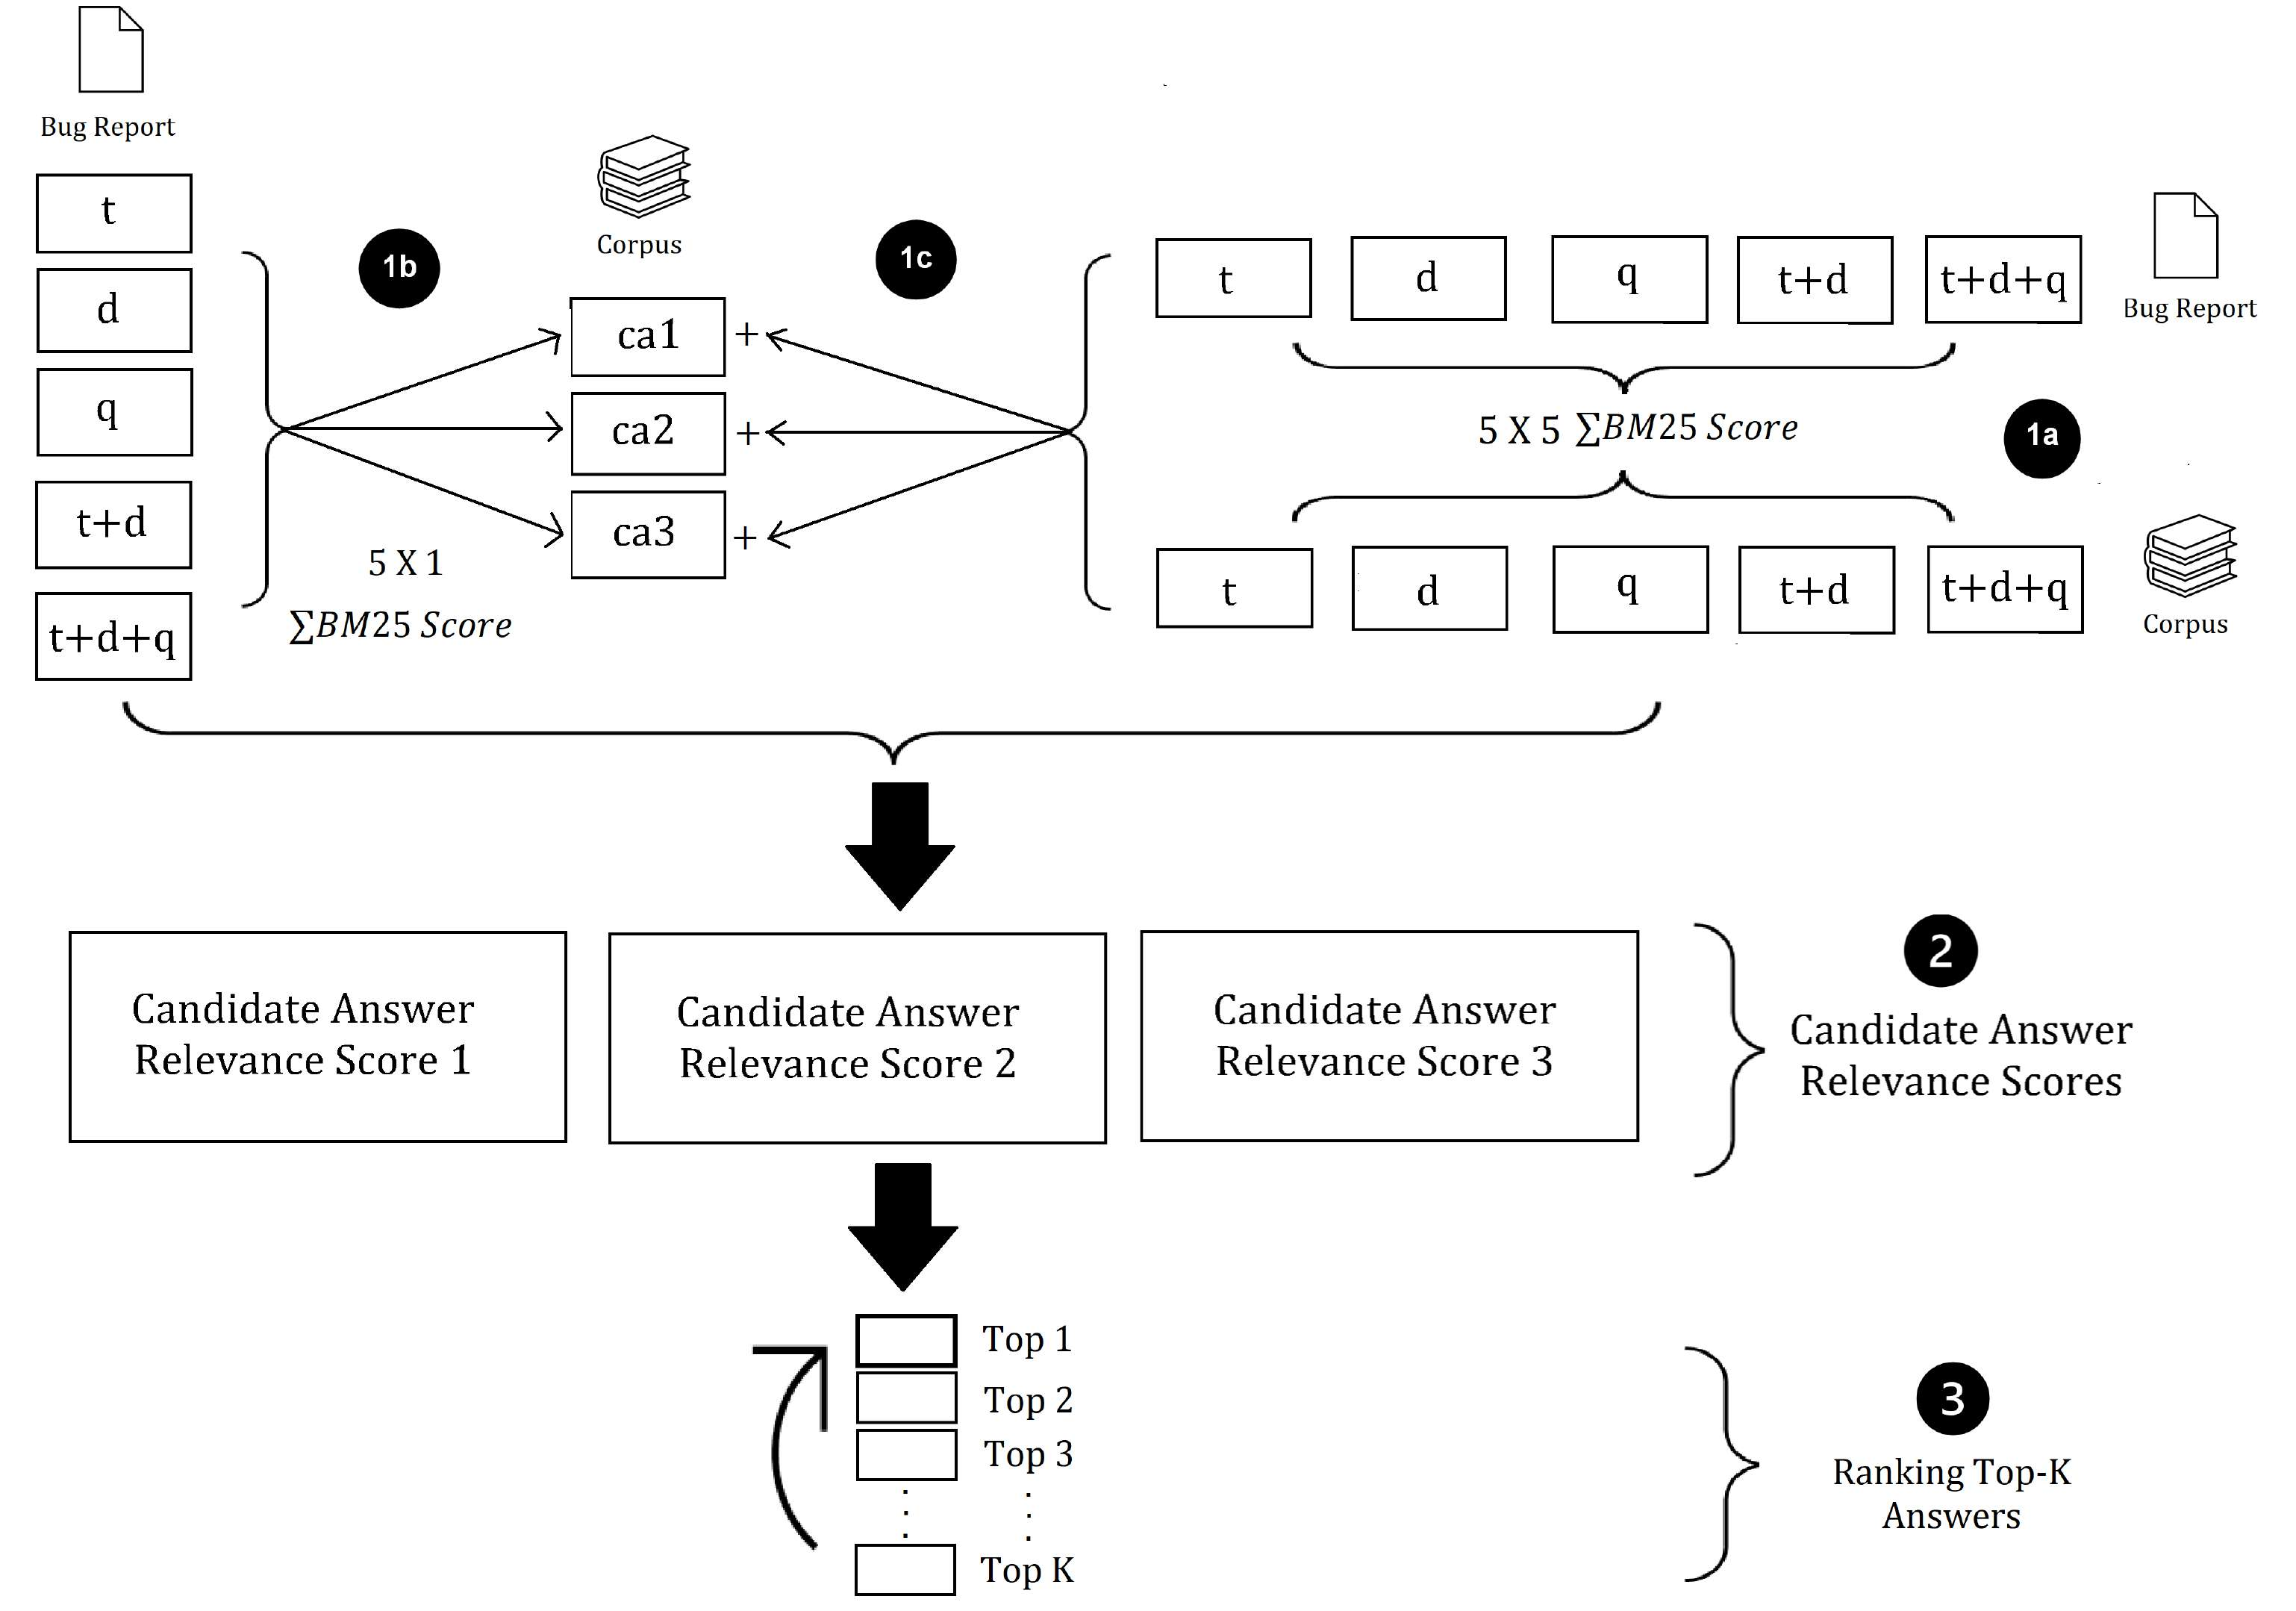
\includegraphics[width=\textwidth, height = 3.5in]{images/Capturing_Relevant_QA_Optimized.pdf}
	% \vspace{-.4cm}
	\caption{Capturing relevant answers with structured Information Retrieval}
	% \vspace{-.6cm}
	\label{fig:qa}
 	% \vspace{-.cm}
\end{figure}
% \\where t-title, d-description, q-question, ca1-candidate answer 1, ca2-candidate answer 2 and ca3-candidate answer 3
\subsubsection{Detecting Relevant Candidate Answers}
\looseness=-1
First, we capture five items from each of the given and past bug reports --- title (t), description (d), follow-up question (q), title + description (t+d), and title + description + question (t+d+q). Then we conduct 25 (5x5) similarity calculations between these bug reports using Eq~\ref{bluir}, and add all 25 similarity scores as shown in Step 1a in Fig.~\ref{fig:qa}. According to existing literature~\cite{saha2013improving}, such an element-based similarity calculation can help prevent spurious matching. This score indicates the general relevance between a given and past bug reports.\par
\looseness=-1
Second, we capture five items from the given bug report --- title (t), description (d), and follow-up question (q), title + description (t+d), and title + description + question (t+d+q) and three candidate answers (ca1, ca2, ca3) from each past bug report. Then, we conduct 5 (5x1) similarity calculations using Eq.~\ref{bluir}, for each of the three candidate answers, as shown in Step 1b, in Fig.~\ref{fig:qa}. This score indicates the relevance between the follow-up question (and its bug report) and each candidate answer.\par

While the score from Step 1a indicates a general relevance between bug reports, the score from Step 1b measures more granular relevance between the question and answer. Thus, the above two scores capture relevance from two different aspects that could be complementary to each other. We thus combine the scores from Step 1a and Step 1b to determine the relevance of each answer against the given follow-up question (and corresponding bug report) in Step 1c.\par

\subsubsection{Ranking Based on Textual Relevance}
We rank the candidate answers based on their BM25-based relevance scores calculated above (Steps 1-2, Fig.~\ref{fig:qa}). In particular, we capture the top K (e.g., 5) relevant candidate answers from the corpus against a follow-up question (Steps 3, Fig.~\ref{fig:qa}). It should be noted that these answers can come from various bug reports.\par

\subsubsection{Ranking Based on Semantic Relevance}
\looseness=-1
BM25 algorithm relies on keyword matching for relevance estimation, which could suffer from the vocabulary mismatch problem~\cite{furnas1987vocabulary}. We thus incorporate embedding-based similarity into our approach and detect the semantically relevant candidate answers. We capture word embeddings, trained by Word2Vec~\cite{church2017word2vec} on Stack Overflow~\cite{efstathiou2018word}, and calculate the cosine similarity between the embeddings of the follow-up question and that of each candidate answer. We then re-rank the answers based on their semantic relevance to the question and return the top K answers.\par

\subsubsection{Capturing the Top Relevant Answers}
\looseness=-1
We combine both BM25-based ranking and semantic relevance-based ranking using the Degree of Interest (DOI) method. Rahman et al.~\cite{rahman2016rack} use the following formulae to combine two orthogonal rankings:\par

\begin{equation}
DOI = \frac{I}{N} 
\end{equation}

\looseness=-1
Here, $I$ is the position of an answer in the ranked list and $N$ is the total number of answers. First, we calculate the DOI score of each answer within the BM25-based list and then, we calculate the DOI score within the semantic relevance-based ranked list. Then we combined the DOI scores for each answer and rank the answers based on their combined DOI score.\par

\subsection{Constructing the Context}
\looseness=-1
Generative question-answering models such as CodeT5 rely on \textit{context} to comprehensively understand the semantics or intent of a question and to generate an answer to the question~\cite{huggingfacegenerativeqa,seonwoo2020context}. We thus construct the context to enrich our follow-up question (Step 3, Fig~\ref{fig:algo}).
To construct the context, we use three items from the previous step --- one answer from the ranked list, its bug report, and the given bug report. The answer and its bug report are likely to contain additional information to compensate for the missing information in the given bug report that triggers a follow-up question. We repeat the context construction for each of the K candidate answers and send them to our CodeT5 model for final answers.\par 

\subsection{Generating Relevant Answers}
\looseness=-1
We then generate relevant answers to the follow-up question by leveraging our context above with CodeT5, a pre-trained encoder-decoder Transformer model for neural text generation. CodeT5 has been pre-trained on  8.35M methods from open-source code accompanied by documentation and adopts an encoder-decoder network to generate texts~\cite{wang2021codet5} (Step 3, Fig~\ref{fig:algo}). The model requires two components to operate, a question and its context. We provide the model with a follow-up question and its context from the previous step and capture an answer to the follow-up question from the model. For example, our technique --- BugMentor --- offers the following answer against the example question in Fig.~\ref{fig:motivating_example}.\par

\FrameSep.3em
\begin{frshaded}
\noindent	
\textbf{Generated Answer: }Adding two flags to Xcode's `Other Linker Flags' settings and modify the Podfile to use the nightly TensorFlow build, specifically `TensorFlowLiteSwift' and `TensorFlowLiteSelectTfOps'
\end{frshaded}



\section{Experiment} \label{Chap1:Experiment}
\looseness=-1
We curated a large dataset containing 30,869 bug reports and their follow-up questions from 20 subject systems and evaluate BugMentor using four appropriate metrics from relevant literature --- BLEU~\cite{papineni2002bleu}, METEOR ~\cite{banerjee2005meteor}, Semantic Similarity~\cite{haque2022semantic} and WMD~\cite{huang2016supervised}. To place our work in the literature, we also conduct an ablation study~\cite{mccandless2010lucene,wang2021codet5} and compare our technique with three baseline techniques. %abalation~\cite{mccandless2010lucene,wang2021codet5}. 
Through our experiments, we answer four research questions as follows:
\begin{enumerate}
\item[(a)] \textbf{RQ$\mathbf{_1}$}: How does our technique perform in answering follow-up questions in terms of different automatic evaluation metrics?
\item[(b)] \textbf{RQ$\mathbf{_2}$}: Can our technique outperform the existing baselines in terms of automatic evaluation metrics?
\item[(c)]\textbf{RQ$\mathbf{_3}$}: How do different components impact the overall performance of BugMentor?
\item[(d)]\textbf{RQ$\mathbf{_4}$}: How accurate, precise, useful, and concise are the answers from BugMentor?
\end{enumerate}

% \subsection{Dataset Collection}

% \subsection{Feasibility Study}
% To investigate the feasibility of our study, we manually examined 450 bug reports comprising of 30 most recent bug reports from 15 different repositories with a high number of issues and forks. Our examination focused on evaluating the quality of the follow-up questions and the received answers.\par
% During our analysis, we observed that many follow-up questions were generic in nature and existing answers to these questions were frequently present in the comments of previous bug reports, duplicate or similar bug reports. Although the answers were not completely syntactically similar, they provided additional information.\par

\subsection{Dataset Construction}\label{sec:dataset-cons}
\subsubsection{Corpus Creation}

\looseness=-1
To construct our corpus, we chose the top 20 popular projects from GitHub written in 4 different programming languages and collected 30,869 bug reports from them. We also capture a follow-up question and three candidate answers from each bug report. Finally, our corpus consisted of hundreds of bug reports where we capture the Bug ID, title, description, follow-up question and three candidate answers from each bug report. We apply standard natural language pre-processing to each item from our corpus. Please check Section~\ref{sec:corpus-construction} for further details on corpus construction.\par

\subsubsection{Ground-Truth Construction}
\label{sec:groundtruth}

\looseness=-1
To evaluate BugMentor, we first construct a randomly sampled held-out dataset (i.e., 95\% confidence level and 4.06\% error margin) containing 550 bug reports ($\sim$27 bug reports x 20 systems). We then involve six human annotators (e.g., graduate students) to determine the ground truth answers against the follow-up question from each bug report. We divided 550 bug reports into six buckets (Table~\ref{tab:interannotatoragreement}), each containing $\sim$90 bug reports, their questions, and candidate answers. Each bucket was annotated by three annotators, resulting in $\sim$270-275 bug reports per annotator. We used majority voting ~\cite{kuhrmann2017pragmatic} to determine the ground truth answers. That is, the answer having the majority of votes was chosen as the ground truth answer against a follow-up question. When the answers did not have a clear majority, i.e. for 3\% of the dataset, the three annotators engaged in discussions to resolve conflicts and determine the ground truth answer~\cite{kuhrmann2017pragmatic}. Each annotator spent $\sim$2.5-3 hours to complete the annotation. \par

\looseness=-1
We compute the Cohen's \emph{$\kappa$} for all pairs of annotators, and the result is reported in Table~\ref{tab:interannotatoragreement}. Although we use majority voting for annotation, our calculated metrics show the agreement level for each pair of annotators. We found an average of 0.46, which indicates a moderate agreement between any two annotators.\par

\begin{table*}[!t]
\centering
\caption{Inter-annotator Agreement}
\label{tab:interannotatoragreement}
\resizebox{\textwidth}{!}{
\begin{tabular}{|cc|cc|cc|cc|cc|cc|}
\hline
\multicolumn{2}{|c|}{\textbf{Bucket 1}}     & \multicolumn{2}{c|}{\textbf{Bucket 2}}     & \multicolumn{2}{c|}{\textbf{Bucket 3}}     & \multicolumn{2}{c|}{\textbf{Bucket 4}}     & \multicolumn{2}{c|}{\textbf{Bucket 5}}     & \multicolumn{2}{c|}{\textbf{Bucket 6}}     \\ \hline
\multicolumn{1}{|c|}{\textbf{Pairs}} & \textbf{$\kappa$}    & \multicolumn{1}{c|}{\textbf{Pairs}} & \textbf{$\kappa$}    & \multicolumn{1}{c|}{\textbf{Pairs}} & \textbf{$\kappa$}    & \multicolumn{1}{c|}{\textbf{Pairs}} & \textbf{$\kappa$}    & \multicolumn{1}{c|}{\textbf{Pairs}} & \textbf{$\kappa$}    & \multicolumn{1}{c|}{\textbf{Pairs}} & \textbf{$\kappa$}    \\ \hline \hline
\multicolumn{1}{|c|}{A1 \& A2}       & 0.72 & \multicolumn{1}{c|}{A2 \& A3}       & 0.58 & \multicolumn{1}{c|}{A3 \& A4}       & 0.44 & \multicolumn{1}{c|}{A4 \& A5}       & 0.66 & \multicolumn{1}{c|}{A5 \& A6}       & 0.49 & \multicolumn{1}{c|}{A1 \& A2}       & 0.41 \\ \hline
\multicolumn{1}{|c|}{A2 \& A3}       & 0.24 & \multicolumn{1}{c|}{A3 \& A4}       & 0.43 & \multicolumn{1}{c|}{A4 \& A5}       & 0.53 & \multicolumn{1}{c|}{A5 \& A6}       & 0.40 & \multicolumn{1}{c|}{A1 \& A5}       & 0.44 & \multicolumn{1}{c|}{A2 \& A6}       & 0.29 \\ \hline
\multicolumn{1}{|c|}{A3 \& A1}       & 0.39 & \multicolumn{1}{c|}{A4 \& A2}       & 0.58 & \multicolumn{1}{c|}{A5 \& A3}       & 0.65 & \multicolumn{1}{c|}{A6 \& A4}       & 0.27 & \multicolumn{1}{c|}{A6 \& A1}       & 0.49 & \multicolumn{1}{c|}{A6 \& A1}       & 0.40 \\ \hline
\end{tabular}}
\end{table*}


\subsection{Evaluation Metrics}

\looseness=-1
To evaluate BugMentor's answers against the ground truth, we use four relevant metrics from literature --- BLEU Score~\cite{papineni2002bleu}, METEOR Score~\cite{banerjee2005meteor}, Word Mover's Distance~\cite{huang2016supervised} and Semantic Similarity metric~\cite{haque2022semantic}. They are defined as follows:\par


\subsubsection{\emph{\textit{1) BLEU --- Bi-Lingual Evaluation of Understudy: }}}
\looseness=-1
\acrshort{BLEU} score is a commonly used metric for evaluating translation~\cite{papineni2002bleu}, which has found application in many software engineering tasks (e.g., comment generation \cite{hu2020deep}). It compares a candidate text to a reference text and determines how similar they are based on the matching of their n-grams. The \acrshort{BLEU} score is calculated as follows:\par

\begin{equation}
BLEU = BP \cdot exp \left ( \sum_{n=1}^{N}w_{n}log(p_{n}) \right )
\end{equation}

where $N$ is the maximum n-gram order, $w\textsubscript{n}$ is the weight assigned to the n-gram order, $BP$ is the brevity penalty - a factor that penalizes the \acrshort{BLEU} score when the candidate text is shorter than the reference text and $p\textsubscript{n}$ is the modified n-gram precision, which measures the ratio of the overlapping n-grams (between the candidate text and the reference text), and the total number of n-grams in the candidate text.\par



\subsubsection{\emph{ \textit{2) METEOR --- Metric for Evaluation of Translation with Explicit ORdering: }}}
\looseness=-1
The \acrshort{METEOR} score is a metric for evaluating the quality of machine translation output based on both lexical and syntactic information~\cite{banerjee2005meteor}. It measures the similarity between a candidate text and the reference text by sequentially applying exact match, stemmed match and wordnet-based synonym match between the texts. 


\subsubsection{\emph{\textit{3) WMD --- Word Mover's Distance: }}}
\looseness=-1
\acrshort{WMD} ~\cite{huang2016supervised} is a similarity measure between two texts based on the meaning or relationships between their words. It is the minimum cost to transform one text into another by calculating the  Euclidean distance between their word embeddings. 



\subsubsection{\emph{\textit{4) SS --- Semantic Similarity: }}}

\looseness=-1
In a recent work, Haque et al.~\cite{haque2022semantic} investigate which metric reflects human assessment of similarity the best. They suggest that Sentence-BERT~\cite{reimers2019sentence} provides semantically meaningful sentence embeddings. Thus when a candidate text is compared with the reference text based on these embeddings using cosine-similarity, it has the highest correlation with human-evaluated similarity. Semantic similarity is computed as follows:

\begin{equation}
SemSim(ref, gen) = \cos(\text{sbert}(ref), \text{sbert}(gen))  
\end{equation}

where $sbert(ref)$, $sbert(gen)$ are the numerical representations from Sentence-BERT for the reference text and generated text respectively.\par

\section{Evaluation of BugMentor} \label{Chap1:Evaluation}
\label{sec:evaluation}


\subsection{Answering RQ$\mathbf{_1}$ --- How does our technique perform in answering follow-up questions in terms of different automatic evaluation metrics?}

In this experiment, we analyze the performance of BugMentor using four different evaluation metrics - \acrshort{BLEU} score~\cite{papineni2002bleu}, \acrlong{Semantic Similarity} ~\cite{haque2022semantic}, \acrshort{METEOR}~\cite{banerjee2005meteor} and WMD~\cite{huang2016supervised}. We divide our held-out dataset into four subsets based on their corresponding programming languages and report the results for each subset. Table~\ref{tab:bugmentorcontext2} shows the performance details of BugMentor in various settings - within the project and cross-project. It should be noted that a higher value for \acrshort{BLEU}, \acrshort{METEOR}, and \acrlong{Semantic Similarity} and a lower value for \acrshort{WMD} metrics are desirable in our experiments.\par

% hybrid - context 2
\renewcommand{\arraystretch}{1.1}
\begin{table*}[!ht]
\centering
\caption{Performance of BugMentor}
\label{tab:bugmentorcontext2}
\resizebox{0.8\textwidth}{!}{%
\begin{tabular}{|ccccccc|}
\hline
\multicolumn{1}{|c|}{\textbf{Metrics}} & \multicolumn{1}{c|}{\textbf{Top K}} & \multicolumn{1}{c|}{\textbf{Python}} & \multicolumn{1}{c|}{\textbf{Java}} & \multicolumn{1}{c|}{\textbf{JavaScript}} & \multicolumn{1}{c|}{\textbf{C++}} & \textbf{Whole Dataset} \\ \hline \hline
\multicolumn{7}{|c|}{\textbf{Within Project}} \\ \hline \hline
\multicolumn{1}{|c|}{\multirow{3}{*}{\textbf{BLEU $\uparrow$}}} & \multicolumn{1}{c|}{Top 1} & \multicolumn{1}{c|}{26.20} & \multicolumn{1}{c|}{22.36} & \multicolumn{1}{c|}{26.06} & \multicolumn{1}{c|}{25.73} & 24.47 \\ \cline{2-7} 
\multicolumn{1}{|c|}{} & \multicolumn{1}{c|}{Top 3} & \multicolumn{1}{c|}{29.25} & \multicolumn{1}{c|}{32.70} & \multicolumn{1}{c|}{31.76} & \multicolumn{1}{c|}{28.03} & 28.90 \\ \cline{2-7} 
\multicolumn{1}{|c|}{} & \multicolumn{1}{c|}{Top 5} & \multicolumn{1}{c|}{34.12} & \multicolumn{1}{c|}{33.82} & \multicolumn{1}{c|}{32.38} & \multicolumn{1}{c|}{30.25} & 31.94 \\ \hline
\multicolumn{1}{|c|}{\multirow{3}{*}{\textbf{METEOR $\uparrow$}}} & \multicolumn{1}{c|}{Top 1} & \multicolumn{1}{c|}{0.14} & \multicolumn{1}{c|}{0.24} & \multicolumn{1}{c|}{0.30} & \multicolumn{1}{c|}{0.21} & 0.24 \\ \cline{2-7} 
\multicolumn{1}{|c|}{} & \multicolumn{1}{c|}{Top 3} & \multicolumn{1}{c|}{0.23} & \multicolumn{1}{c|}{0.26} & \multicolumn{1}{c|}{0.34} & \multicolumn{1}{c|}{0.26} & 0.36 \\ \cline{2-7} 
\multicolumn{1}{|c|}{} & \multicolumn{1}{c|}{Top 5} & \multicolumn{1}{c|}{0.29} & \multicolumn{1}{c|}{0.57} & \multicolumn{1}{c|}{0.36} & \multicolumn{1}{c|}{0.29} & 0.42 \\ \hline
\multicolumn{1}{|c|}{\multirow{3}{*}{\textbf{SS $\uparrow$}}} & \multicolumn{1}{c|}{Top 1} & \multicolumn{1}{c|}{43.20} & \multicolumn{1}{c|}{42.90} & \multicolumn{1}{c|}{46.30} & \multicolumn{1}{c|}{46.13} & 50.63 \\ \cline{2-7} 
\multicolumn{1}{|c|}{} & \multicolumn{1}{c|}{Top 3} & \multicolumn{1}{c|}{58.80} & \multicolumn{1}{c|}{42.90} & \multicolumn{1}{c|}{45.50} & \multicolumn{1}{c|}{54.30} & 53.49 \\ \cline{2-7} 
\multicolumn{1}{|c|}{} & \multicolumn{1}{c|}{Top 5} & \multicolumn{1}{c|}{64.50} & \multicolumn{1}{c|}{54.70} & \multicolumn{1}{c|}{54.20} & \multicolumn{1}{c|}{56.10} & 57.01 \\ \hline
\multicolumn{1}{|c|}{\multirow{3}{*}{\textbf{WMD $\downarrow$}}} & \multicolumn{1}{c|}{Top 1} & \multicolumn{1}{c|}{5.09} & \multicolumn{1}{c|}{4.97} & \multicolumn{1}{c|}{4.91} & \multicolumn{1}{c|}{5.35} & 4.18 \\ \cline{2-7} 
\multicolumn{1}{|c|}{} & \multicolumn{1}{c|}{Top 3} & \multicolumn{1}{c|}{4.89} & \multicolumn{1}{c|}{4.64} & \multicolumn{1}{c|}{4.75} & \multicolumn{1}{c|}{4.93} & 3.80 \\ \cline{2-7} 
\multicolumn{1}{|c|}{} & \multicolumn{1}{c|}{Top 5} & \multicolumn{1}{c|}{4.82} & \multicolumn{1}{c|}{3.27} & \multicolumn{1}{c|}{4.29} & \multicolumn{1}{c|}{4.56} & 3.65 \\ \hline \hline
\multicolumn{7}{|c|}{\textbf{Cross Project}} \\ \hline  \hline
\multicolumn{1}{|c|}{\multirow{3}{*}{\textbf{BLEU $\uparrow$}}} & \multicolumn{1}{c|}{Top 1} & \multicolumn{1}{c|}{16.71} & \multicolumn{1}{c|}{14.24} & \multicolumn{1}{c|}{12.36} & \multicolumn{1}{c|}{16.03} & 14.84 \\ \cline{2-7} 
\multicolumn{1}{|c|}{} & \multicolumn{1}{c|}{Top 3} & \multicolumn{1}{c|}{20.52} & \multicolumn{1}{c|}{15.12} & \multicolumn{1}{c|}{16.99} & \multicolumn{1}{c|}{18.97} & 17.90 \\ \cline{2-7} 
\multicolumn{1}{|c|}{} & \multicolumn{1}{c|}{Top 5} & \multicolumn{1}{c|}{21.86} & \multicolumn{1}{c|}{17.70} & \multicolumn{1}{c|}{19.30} & \multicolumn{1}{c|}{19.92} & 19.70 \\ \hline
\multicolumn{1}{|c|}{\multirow{3}{*}{\textbf{METEOR $\uparrow$}}} & \multicolumn{1}{c|}{Top 1} & \multicolumn{1}{c|}{0.12} & \multicolumn{1}{c|}{0.13} & \multicolumn{1}{c|}{0.11} & \multicolumn{1}{c|}{0.09} & 0.11 \\ \cline{2-7} 
\multicolumn{1}{|c|}{} & \multicolumn{1}{c|}{Top 3} & \multicolumn{1}{c|}{0.14} & \multicolumn{1}{c|}{0.16} & \multicolumn{1}{c|}{0.13} & \multicolumn{1}{c|}{0.11} & 0.14 \\ \cline{2-7} 
\multicolumn{1}{|c|}{} & \multicolumn{1}{c|}{Top 5} & \multicolumn{1}{c|}{0.15} & \multicolumn{1}{c|}{0.19} & \multicolumn{1}{c|}{0.14} & \multicolumn{1}{c|}{0.12} & 0.15 \\ \hline
\multicolumn{1}{|c|}{\multirow{3}{*}{\textbf{SS $\uparrow$}}} & \multicolumn{1}{c|}{Top 1} & \multicolumn{1}{c|}{26.80} & \multicolumn{1}{c|}{26.23} & \multicolumn{1}{c|}{27.76} & \multicolumn{1}{c|}{27.30} & 27.02 \\ \cline{2-7} 
\multicolumn{1}{|c|}{} & \multicolumn{1}{c|}{Top 3} & \multicolumn{1}{c|}{29.15} & \multicolumn{1}{c|}{29.52} & \multicolumn{1}{c|}{29.75} & \multicolumn{1}{c|}{29.27} & 29.42 \\ \cline{2-7} 
\multicolumn{1}{|c|}{} & \multicolumn{1}{c|}{Top 5} & \multicolumn{1}{c|}{31.89} & \multicolumn{1}{c|}{31.80} & \multicolumn{1}{c|}{30.93} & \multicolumn{1}{c|}{30.75} & 31.34 \\ \hline
\multicolumn{1}{|c|}{\multirow{3}{*}{\textbf{WMD $\downarrow$}}} & \multicolumn{1}{c|}{Top 1} & \multicolumn{1}{c|}{5.23} & \multicolumn{1}{c|}{5.62} & \multicolumn{1}{c|}{5.10} & \multicolumn{1}{c|}{5.43} & 5.34 \\ \cline{2-7} 
\multicolumn{1}{|c|}{} & \multicolumn{1}{c|}{Top 3} & \multicolumn{1}{c|}{5.02} & \multicolumn{1}{c|}{5.64} & \multicolumn{1}{c|}{5.01} & \multicolumn{1}{c|}{5.38} & 5.26 \\ \cline{2-7} 
\multicolumn{1}{|c|}{} & \multicolumn{1}{c|}{Top 5} & \multicolumn{1}{c|}{4.87} & \multicolumn{1}{c|}{5.68} & \multicolumn{1}{c|}{4.98} & \multicolumn{1}{c|}{5.36} & 5.22 \\ \hline
\end{tabular}%
}
\end{table*}

\looseness=-1
BugMentor achieves an average BLEU Score of 24.47 for Top 1 answer, and a maximum of 31.94 for Top 5 answers when our whole dataset is considered. In the case of cross-project setting, these scores drop to 14.84 and 19.70, respectively. However, our technique achieves a maximum of 26.20 for the Top 1, 32.7 for Top 3 and 34.12 for Top 5 answers across all four subsets. These BLEU scores indicate that our generated answers are \textit{understandable} and \textit{good} according to Google’s AutoML Translation documentation~\cite{automldoc}. This also shows that the answers generated by BugMentor have a significant overlap with the ground truth in terms of words and word order. However, BLEU score primarily focuses on capturing the precision of an answer against the ground truth. Hence we also evaluate our answers using the METEOR score, where recall is captured by taking into account additional information such as synonyms, word forms, and sentence structure ~\cite{banerjee2005meteor}.\par

As shown in Table~\ref{tab:bugmentorcontext2}, BugMentor achieves an average METEOR score of 0.24 for Top 1 answer, and a maximum of 0.42 for Top 5 answers against the whole dataset, which are considered to be reasonable~\cite{agarwal2008meteor}. In cross-project setting, our technique achieves an average METEOR score of 0.11 for Top 1 answer, and a maximum of 0.15 for Top 5 answers. It achieves a maximum of 0.30 for Top 1, 0.34 for Top 3, and 0.57 for Top 5 answers across four subsets. This shows that BugMentor was able to produce a significant part of the ground truth texts in the generated answers. However, since BLEU and METEOR scores rely on keyword matching between a generated answer and the ground truth answer, they may not capture the semantic relevance between them. Hence we also evaluate our technique using WMD~\cite{huang2016supervised} and Semantic Similarity~\cite{haque2022semantic}. They also have been shown to correlate better with human judgement of relevance ~\cite{papineni2002bleu, kusner2015word}. \par

\looseness=-1
In Table~\ref{tab:bugmentorcontext2}, we find that BugMentor achieves an average WMD of 4.18 for Top 1 answer, and a minimum of 3.65 for Top 5 answers, when the whole dataset is considered. In cross-project setting, our technique achieves an average WMD of 5.34 for Top 1 answer, and a minimum of 5.22 for Top 5 answers. These distance scores show that BugMentor was able to generate answers semantically similar to the ground truth and were worded closely to the ground truth. However, WMD may not be sufficient to reflect the importance and context of words in a sentence ~\cite{kusner2015word,sato2022re}. We thus also evaluate our answers using semantic similarity against the ground truth. The metric is appropriate when there may not be any syntactic overlap between the answers, which is a common phenomenon in question answering, according to existing literature ~\cite{yao2013answer,severyn2015learning}.\par

\looseness=-1
From Table ~\ref{tab:bugmentorcontext2}, we also find that the answers from BugMentor have an average Semantic Similarity score of  50.63\% for Top 1 answer, and a maximum of 57.01\% for Top 5 answers when the whole dataset is considered. It achieves an average Semantic Similarity score of 27.02\% for Top 1 answer, and a maximum 31.34\% for Top 5 answer in cross-project setting. BugMentor achieves a maximum of 46.13\% for Top 1, and a maximum of 64.5\% for Top 5 answers when all subsets are considered. All these numbers indicate a high similarity in meaning and content between BugMentor's answers and the ground truth.\par


\FrameSep.3em
\begin{frshaded}
	\noindent
	\textbf{Summary of RQ$\mathbf{_1}$:} BugMentor can generate relevant answers to follow-up questions that are \textit{understandable} to \textit{good} according to Google's Standard and achieves an average BLEU score of 31.94. Its answers also have a high semantic overlap with the ground truth answers and thus achieve an average semantic similarity score of 57\%.
\end{frshaded}

\subsection{Answering RQ$\mathbf{_2}$ --- Can our technique outperform the existing baselines in terms of automatic evaluation metrics?}\label{results:rq2}

To the best of our knowledge, there exists no work that can offer relevant answers to follow-up questions from bug reports. However, Lucene~\cite{mccandless2010lucene} is a popular IR-based tool that has been used to recommend answers in the programming Q\&A site ~\cite{Atwood_2017,ponzanelli2013leveraging}.
CodeT5~\cite{wang2021codet5} is a large language model for generating answers to questions. AnswerBot~\cite{xu2017answerbot} can synthesize
answers for technical, non-factoid questions on StackOverflow. We thus consider them as our baselines for the comparison. We call them Baseline$_{Lucene}$, Baseline$_{CodeT5}$ and AnswerBot, respectively in this experiment. We evaluate the answers from all three baselines against the ground truth using four evaluation metrics. Tables~\ref{tab:baselinecomparison1} and ~\ref{tab:baselinecomparison2} show the comparison details between BugMentor and these baseline techniques.\par

\begin{table*}[!ht]
\centering
\caption{Comparison of BugMentor with Baseline$_{Lucene}$ and Answerbot}
\label{tab:baselinecomparison1}
\resizebox{0.7\textwidth}{!}{%
    \begin{tabular}{|ccccc|}
    \hline
    \multicolumn{1}{|c|}{\textbf{Metrics}} & \multicolumn{1}{c|}{\textbf{Top K}} & \multicolumn{1}{c|}{\textbf{AnswerBot}} & \multicolumn{1}{c|}{\textbf{Baseline$_{Lucene}$}} & \textbf{BugMentor} \\ \hline \hline
    \multicolumn{1}{|c|}{\multirow{3}{*}{\textbf{BLEU $\uparrow$}}} & \multicolumn{1}{c|}{Top 1} & \multicolumn{1}{c|}{4.31} & \multicolumn{1}{c|}{8.60} & \textbf{24.47} \\ \cline{2-5} 
    \multicolumn{1}{|c|}{} & \multicolumn{1}{c|}{Top 3} & \multicolumn{1}{c|}{6.71} & \multicolumn{1}{c|}{10.54} & \textbf{28.9} \\ \cline{2-5} 
    \multicolumn{1}{|c|}{} & \multicolumn{1}{c|}{Top 5} & \multicolumn{1}{c|}{4.24} & \multicolumn{1}{c|}{14.31} & \textbf{31.94} \\ \hline
    \multicolumn{1}{|c|}{\multirow{3}{*}{\textbf{METEOR $\uparrow$}}} & \multicolumn{1}{c|}{Top 1} & \multicolumn{1}{c|}{0.05} & \multicolumn{1}{c|}{0.18} & \textbf{0.24} \\ \cline{2-5} 
    \multicolumn{1}{|c|}{} & \multicolumn{1}{c|}{Top 3} & \multicolumn{1}{c|}{0.12} & \multicolumn{1}{c|}{0.19} & \textbf{0.36} \\ \cline{2-5} 
    \multicolumn{1}{|c|}{} & \multicolumn{1}{c|}{Top 5} & \multicolumn{1}{c|}{0.07} & \multicolumn{1}{c|}{0.21} & \textbf{0.42} \\ \hline
    \multicolumn{1}{|c|}{\multirow{3}{*}{\textbf{SS $\uparrow$}}} & \multicolumn{1}{c|}{Top 1} & \multicolumn{1}{c|}{36.47} & \multicolumn{1}{c|}{42.75} & \textbf{50.63} \\ \cline{2-5} 
    \multicolumn{1}{|c|}{} & \multicolumn{1}{c|}{Top 3} & \multicolumn{1}{c|}{47.69} & \multicolumn{1}{c|}{45.45} & \textbf{53.49} \\ \cline{2-5} 
    \multicolumn{1}{|c|}{} & \multicolumn{1}{c|}{Top 5} & \multicolumn{1}{c|}{47.69} & \multicolumn{1}{c|}{48.78} & \textbf{57.01} \\ \hline
    \multicolumn{1}{|c|}{\multirow{3}{*}{\textbf{WMD $\downarrow$}}} & \multicolumn{1}{c|}{Top 1} & \multicolumn{1}{c|}{5.7} & \multicolumn{1}{c|}{4.55} & \textbf{4.18} \\ \cline{2-5} 
    \multicolumn{1}{|c|}{} & \multicolumn{1}{c|}{Top 3} & \multicolumn{1}{c|}{4.81} & \multicolumn{1}{c|}{4.46} & \textbf{3.80} \\ \cline{2-5} 
    \multicolumn{1}{|c|}{} & \multicolumn{1}{c|}{Top 5} & \multicolumn{1}{c|}{5.01} & \multicolumn{1}{c|}{4.37} & \textbf{3.65} \\ \hline
    \end{tabular}}
\vspace{1cm} 
    \caption{Comparison of BugMentor with Baseline$_{CodeT5}$}
    \label{tab:baselinecomparison2}
    \resizebox{0.6\textwidth}{!}{%
    \begin{tabular}{|cccc|}
    \hline
    \multicolumn{1}{|c|}{\textbf{Metrics}} & \multicolumn{1}{c|}{\textbf{Top K}} & \multicolumn{1}{c|}{\textbf{Baseline$_{CodeT5}$}} & \textbf{BugMentor} \\ \hline
    \multicolumn{1}{|c|}{\textbf{BLEU $\uparrow$}} & \multicolumn{1}{c|}{\multirow{4}{*}{Top 1}} & \multicolumn{1}{c|}{2.4} & \textbf{24.47} \\ \cline{1-1} \cline{3-4} 
    \multicolumn{1}{|c|}{\textbf{METEOR $\uparrow$}} & \multicolumn{1}{c|}{} & \multicolumn{1}{c|}{0.04} & \textbf{0.24} \\ \cline{1-1} \cline{3-4} 
    \multicolumn{1}{|c|}{\textbf{SS $\uparrow$}} & \multicolumn{1}{c|}{} & \multicolumn{1}{c|}{11.01} & \textbf{50.63} \\ \cline{1-1} \cline{3-4} 
    \multicolumn{1}{|c|}{\textbf{WMD $\downarrow$}} & \multicolumn{1}{c|}{} & \multicolumn{1}{c|}{7.32} & \textbf{4.18} \\ \hline
    \end{tabular}}
\end{table*}

\looseness=-1
To implement Baseline$_{Lucene}$, we provide a follow-up question as the \emph{query} and all candidate answers as the \emph{corpus} to the Lucene tool. Then we collect the top K answers from the tool by executing the query for our evaluation. Baseline$_{Lucene}$ achieves a BLEU score of 8.60, METEOR score of 0.18, Semantic Similarity of 42.75 and WMD of 4.55. On the other hand, BugMentor achieves a BLEU score of 24.47, METEOR score of 0.24, Semantic Similarity of 50.63 and WMD of 4.18. Thus, our technique outperforms the baseline in all four metrics.\par


\looseness=-1
To implement Baseline$_{CodeT5}$, we provide a follow-up question as the \emph{query} and its corresponding bug report as \emph{context} to the CodeT5 model, which generates an answer. We observe that Baseline$_{CodeT5}$ performs significantly poorly when compared to BugMentor and  Baseline$_{Lucene}$. For example, Baseline$_{CodeT5}$ achieves a BLEU score of 2.4, METEOR score of 0.04, Semantic Similarity of 11.01 and WMD of 7.32, which are 42\%-90\% lower than the corresponding measures from BugMentor.


\looseness=-1
To implement AnswerBot, we use the replication package provided by the authors~\cite{xu2017answerbot, maxxbw54}. We provide a follow-up question as the \emph{query} and all bug reports along with their candidate answers as the \emph{corpus}. We observe that AnswerBot performs significantly poorly when compared to BugMentor and  Baseline$_{Lucene}$. For example, AnswerBot achieves a maximum BLEU score of 6.71, METEOR score of 0.12, Semantic Similarity of 47.69 and a minimum WMD of 4.81, which are lower than the corresponding measures from BugMentor.\par


\looseness=-1
We also perform Mann-Whitney Wilcoxon test~\cite{cuzick1985wilcoxon} to check if the performance of Baseline$_{Lucene}$, Baseline$_{CodeT5}$, AnswerBot are significantly lower than that of BugMentor using BonFerroni Correction~\cite{weisstein2004bonferroni}. We find that BugMentor performs significantly higher than Baseline$_{Lucene}$ and AnswerBot, i.e., p-value $=$ 0.010$<$0.016 in terms of all four metrics.\par

Besides the comparison with traditional baselines, it is important to consider the other the competitive landscape, particularly with the emergence of popular Language Model-based approaches (LLMs) such as ChatGPT. Upon conducting a limited qualitative analysis, we observe that while ChatGPT exhibit a profound understanding of the bug report context, they fall short in providing answers to follow-up questions with the desired level of specificity. Furthermore, the responses generated by LLMs tend to be more verbose, lacking the precision found in BugMentor's answers. BugMentor gains a deeper understanding of the bugs from historical bug reports, excels in capturing a broader context, and thus was able to generate more accurate responses to follow-up questions. In future, we plan to extensively compare BugMentor with the modern LLM-based approaches such as ChatGPT.

\FrameSep.3em
\begin{frshaded}
	\noindent
	\textbf{Summary of RQ$\mathbf{_2}$:} BugMentor performs better in answer generation than all three baselines in terms of four evaluation metrics. According to the statistical significance test, BugMentor outperforms the closest competitors Baseline$_{Lucene}$ and AnswerBot  – by a statistically significant margin.
\end{frshaded} 




\subsection{Answering RQ$\mathbf{_3}$ --- How do different components impact the overall performance of BugMentor?}

\looseness=-1
Our technique has three key components --- (a) structured information retrieval, (b) embedding similarity-based ranking and (c) neural text generation. 
In this experiment, we conduct an ablation study to determine the contribution of each component. In particular, we design different variants of BugMentor with each component and evaluate their performance in answer generation. Table~\ref{tab:ablation} summarizes our results from the ablation study.\par


\looseness=-1
We find that BugMentor outperforms all of its variants based on either individual components or their combinations. The combination of structured information retrieval and neural text generation (a.k.a., BugMentor$_{Lucene+CodeT5}$) is a close second when compared using BLEU and Semantic Similarity scores. We see that the absence of the embedding component reduces its performance from that of BugMentor by 3.63\% in terms of BLEU and 10.17\% in terms of Semantic Similarity and increases in WMD by 17.70\% when the Top 1 answer is captured. Thus, the Embedding component improves the semantic closeness between the generated answers and ground truth. \par

\renewcommand{\arraystretch}{1.5}
\begin{table}[!t]
\centering
\caption{Experimental Results from the Ablation Study}
\label{tab:ablation}
\resizebox{\textwidth}{!}{%
\begin{tabular}{|c|c|clccc|}
\hline
\multirow{2}{*}{\textbf{Metrics}} & \multirow{2}{*}{\textbf{Top K}} & \multicolumn{5}{c|}{\textbf{Components}} \\ \cline{3-7} 
 &  & \multicolumn{1}{c|}{\textbf{BugMentor$_{L}$}} & \multicolumn{1}{c|}{\textbf{BugMentor$_{CT5}$}} & \multicolumn{1}{c|}{\textbf{BugMentor$_{L+E}$}} & \multicolumn{1}{c|}{\textbf{BugMentor$_{L+CT5}$}} & \textbf{BugMentor} \\ \hline \hline
\multirow{3}{*}{\textbf{BLEU $\uparrow$}} & Top 1 & \multicolumn{1}{c|}{7.62} & \multicolumn{1}{c|}{2.40} & \multicolumn{1}{c|}{5.65} & \multicolumn{1}{c|}{23.58} & \textbf{24.47} \\ \cline{2-7} 
 & Top 3 & \multicolumn{1}{c|}{12.05} & \multicolumn{1}{l|}{\multirow{2}{*}{}} & \multicolumn{1}{c|}{6.63} & \multicolumn{1}{c|}{30.50} & \textbf{28.90} \\ \cline{2-3} \cline{5-7} 
 & Top 5 & \multicolumn{1}{c|}{19.40} & \multicolumn{1}{l|}{} & \multicolumn{1}{c|}{8.35} & \multicolumn{1}{c|}{33.41} & \textbf{31.94} \\ \hline
\multirow{3}{*}{\textbf{METEOR $\uparrow$}} & Top 1 & \multicolumn{1}{c|}{0.21} & \multicolumn{1}{c|}{0.04} & \multicolumn{1}{c|}{0.28} & \multicolumn{1}{c|}{0.26} & \textbf{0.24} \\ \cline{2-7} 
 & Top 3 & \multicolumn{1}{c|}{0.23} & \multicolumn{1}{l|}{\multirow{2}{*}{}} & \multicolumn{1}{c|}{0.28} & \multicolumn{1}{c|}{0.30} & \textbf{0.36} \\ \cline{2-3} \cline{5-7} 
 & Top 5 & \multicolumn{1}{c|}{0.25} & \multicolumn{1}{l|}{} & \multicolumn{1}{c|}{0.31} & \multicolumn{1}{c|}{0.32} & \textbf{0.42} \\ \hline
\multirow{3}{*}{\textbf{SS $\uparrow$}} & Top 1 & \multicolumn{1}{c|}{50.36} & \multicolumn{1}{c|}{11.01} & \multicolumn{1}{c|}{53.28} & \multicolumn{1}{c|}{45.48} & \textbf{50.63} \\ \cline{2-7} 
 & Top 3 & \multicolumn{1}{c|}{53.96} & \multicolumn{1}{l|}{\multirow{2}{*}{}} & \multicolumn{1}{c|}{53.49} & \multicolumn{1}{c|}{50.38} & \textbf{58.11} \\ \cline{2-3} \cline{5-7} 
 & Top 5 & \multicolumn{1}{c|}{57.09} & \multicolumn{1}{l|}{} & \multicolumn{1}{c|}{60.33} & \multicolumn{1}{c|}{53.69} & \textbf{57.01} \\ \hline
\multirow{3}{*}{\textbf{WMD $\downarrow$}} & Top 1 & \multicolumn{1}{c|}{4.29} & \multicolumn{1}{c|}{7.32} & \multicolumn{1}{c|}{3.97} & \multicolumn{1}{c|}{4.92} & \textbf{4.18} \\ \cline{2-7} 
 & Top 3 & \multicolumn{1}{c|}{4.15} & \multicolumn{1}{l|}{\multirow{2}{*}{}} & \multicolumn{1}{c|}{3.89} & \multicolumn{1}{c|}{4.62} & \textbf{3.80} \\ \cline{2-3} \cline{5-7} 
 & Top 5 & \multicolumn{1}{c|}{4.02} & \multicolumn{1}{l|}{} & \multicolumn{1}{c|}{3.72} & \multicolumn{1}{c|}{4.42} & \textbf{3.65} \\ \hline
\end{tabular}%
}
\begin{tablenotes}
  \small
  \item \begin{center}
     \textbf{BugMentor$_{L}$} $=$ BugMentor$_{Lucene}$, \textbf{BugMentor$_{CT5}$} $=$ BugMentor$_{CodeT5}$,\\
     \textbf{BugMentor$_{L+E}$} $=$ BugMentor$_{Lucene + Embedding}$ ,\\ \textbf{BugMentor$_{L+CT5}$} $=$ BugMentor$_{Lucene+CodeT5}$
  \end{center}
\end{tablenotes}
\end{table}


\looseness=-1
From Table~\ref{tab:ablation}, we also note that the combination of Lucene and Embedding (a.k.a., BugMentor$_{Lucene + Embedding}$) is the closest competitor to BugMentor when BLEU is considered. However, the absence of the text generation component (a.k.a., CodeT5) reduces the performance of the variant by 76.91\% in terms of BLEU. It also shows a decrease in performance by 22.22\% in terms of METEOR, 7.95\% in terms of Semantic Similarity and an increase in WMD by 2.36\% when Top 3 answers are considered. Thus, the CodeT5 component has a significant impact on improving not only the understandability of our generated answers (i.e., BLEU) but also their syntactic and semantic relevance to the ground truth answers (i.e. METEOR, WMD, Semantic Similarity).\par

\looseness=-1
From Table~\ref{tab:ablation}, we also find that the components from BugMentor do not perform well when evaluated individually. For example, if we omit both Embedding and CodeT5 components and only use Lucene, the performance degrades by 68.85\% in terms of BLEU, 12.5\% in terms of METEOR and 0.53\% in terms of Semantic Similarity and WMD increases by 2.63\% for Top 1 answer. Similarly, if we use only the CodeT5 component, the performance degrades by 90.19\% in terms of BLEU, 83.33\% in terms of METEOR and 78.25\% in terms of Semantic Similarity and WMD increases by 75.11\% for Top 1 answer. \par


\FrameSep.3em
\begin{frshaded}
	\noindent
	\textbf{Summary of RQ$\mathbf{_3}$:} Our ablation study demonstrates the contribution of the three components --- structured information retrieval, embedding similarity-based ranking, and neural text generation (a.k.a CodeT5) --- towards the overall performance of BugMentor. We also found that BugMentor outperforms its four variants based on individual components or their combinations, which justifies the presence of all three components in BugMentor.
\end{frshaded} 


\subsection{Answering RQ$\mathbf{_4}$ --- How accurate, precise, useful, and concise are the answers from BugMentor?}

The metric-based evaluation above demonstrates the benefits of our technique in answering follow-up questions using four similarity measures. We conduct a developer study to further demonstrate the benefits of our technique in a practical setting. Given a bug report (e.g., title, description, and follow-up question), we evaluate how \emph{accurate}, \emph{precise}, \emph{useful}, and \emph{concise} (details in Table~\ref{tab:devstudyqualityaspects}) our answers are according to human developers.\par

\begin{table}[ht]
\centering
\caption{Quality Aspects of the Generated Answers}
\label{tab:devstudyqualityaspects}
\renewcommand{\arraystretch}{1.5}
\resizebox{0.8\textwidth}{!}{
\begin{tabular}{|l|l|}
\hline
\textbf{Quality} & \textbf{Overview} \\ \hline \hline
Accurate  & It provides the same factual information as the reference. \\ \hline
Precise & It can answer the question completely \\ \hline
Concise & It is short and still answers the question. \\ \hline
Useful & The provided information has the potential to answer the question. \\ \hline
\end{tabular}}
\end{table}

\textbf{Study Participants:} 
The target group for our study consists of English-speaking software developers with professional experience in four programming languages --- Python, Java, JS, and C++ --- that were used by our collected projects. We sent an open invitation through our personal connections, and 10 graduate students responded to our invitation. Each of them had professional experience in software development and at least two years of experience in the aforementioned programming languages. We provide them with a quick overview of our project using relevant examples and a secured link containing our survey. None of the participants knew the specifics of our designed technique --- BugMentor. \par
% developer study table

\looseness=-1
\textbf{Study Setup:} For our study, we use 12 use cases where each use case consists of a bug report and a follow-up question. To select these use cases, we apply random sampling without replacement to the held-out dataset (Section~\ref{sec:dataset-cons}). To avoid information overload, we select such bug reports that (a) do not have any stack trace information and (b) do not warrant any project-specific knowledge to understand the bug. We select three randomly sampled bug reports from each subset (based on programming language, Section~\ref{sec:dataset-cons}) and collect corresponding follow-up questions, ground truth answers, and the answers from both BugMentor and three baseline techniques --- AnswerBot, Baseline$_{Lucene}$ and Baseline$_{CodeT5}$.\par

\looseness=-1
We present all 12 use cases to each of the participants. Then the participants were instructed to assess the accuracy, precision, usefulness and conciseness of the generated answers (by BugMentor and baselines) with respect to the ground truth answers. We also instruct the participants to submit their evaluation on a five-point Likert scale, where 1 indicates strongly disagree and 5 indicates strongly agree. \textbf{We also anonymize the source of all generated answers to avoid any potential bias towards any of the techniques.}
We thus collect a total of  192 data points (12 questions × 4 explanations × 4 evaluation aspects) from each of the 10 participants.\par

The design of our developer survey has been reviewed and approved by the Dalhousie University Research Ethics Board (REB file \#: 2023-6885).\par

\begin{figure*}[!t]
	\centering
 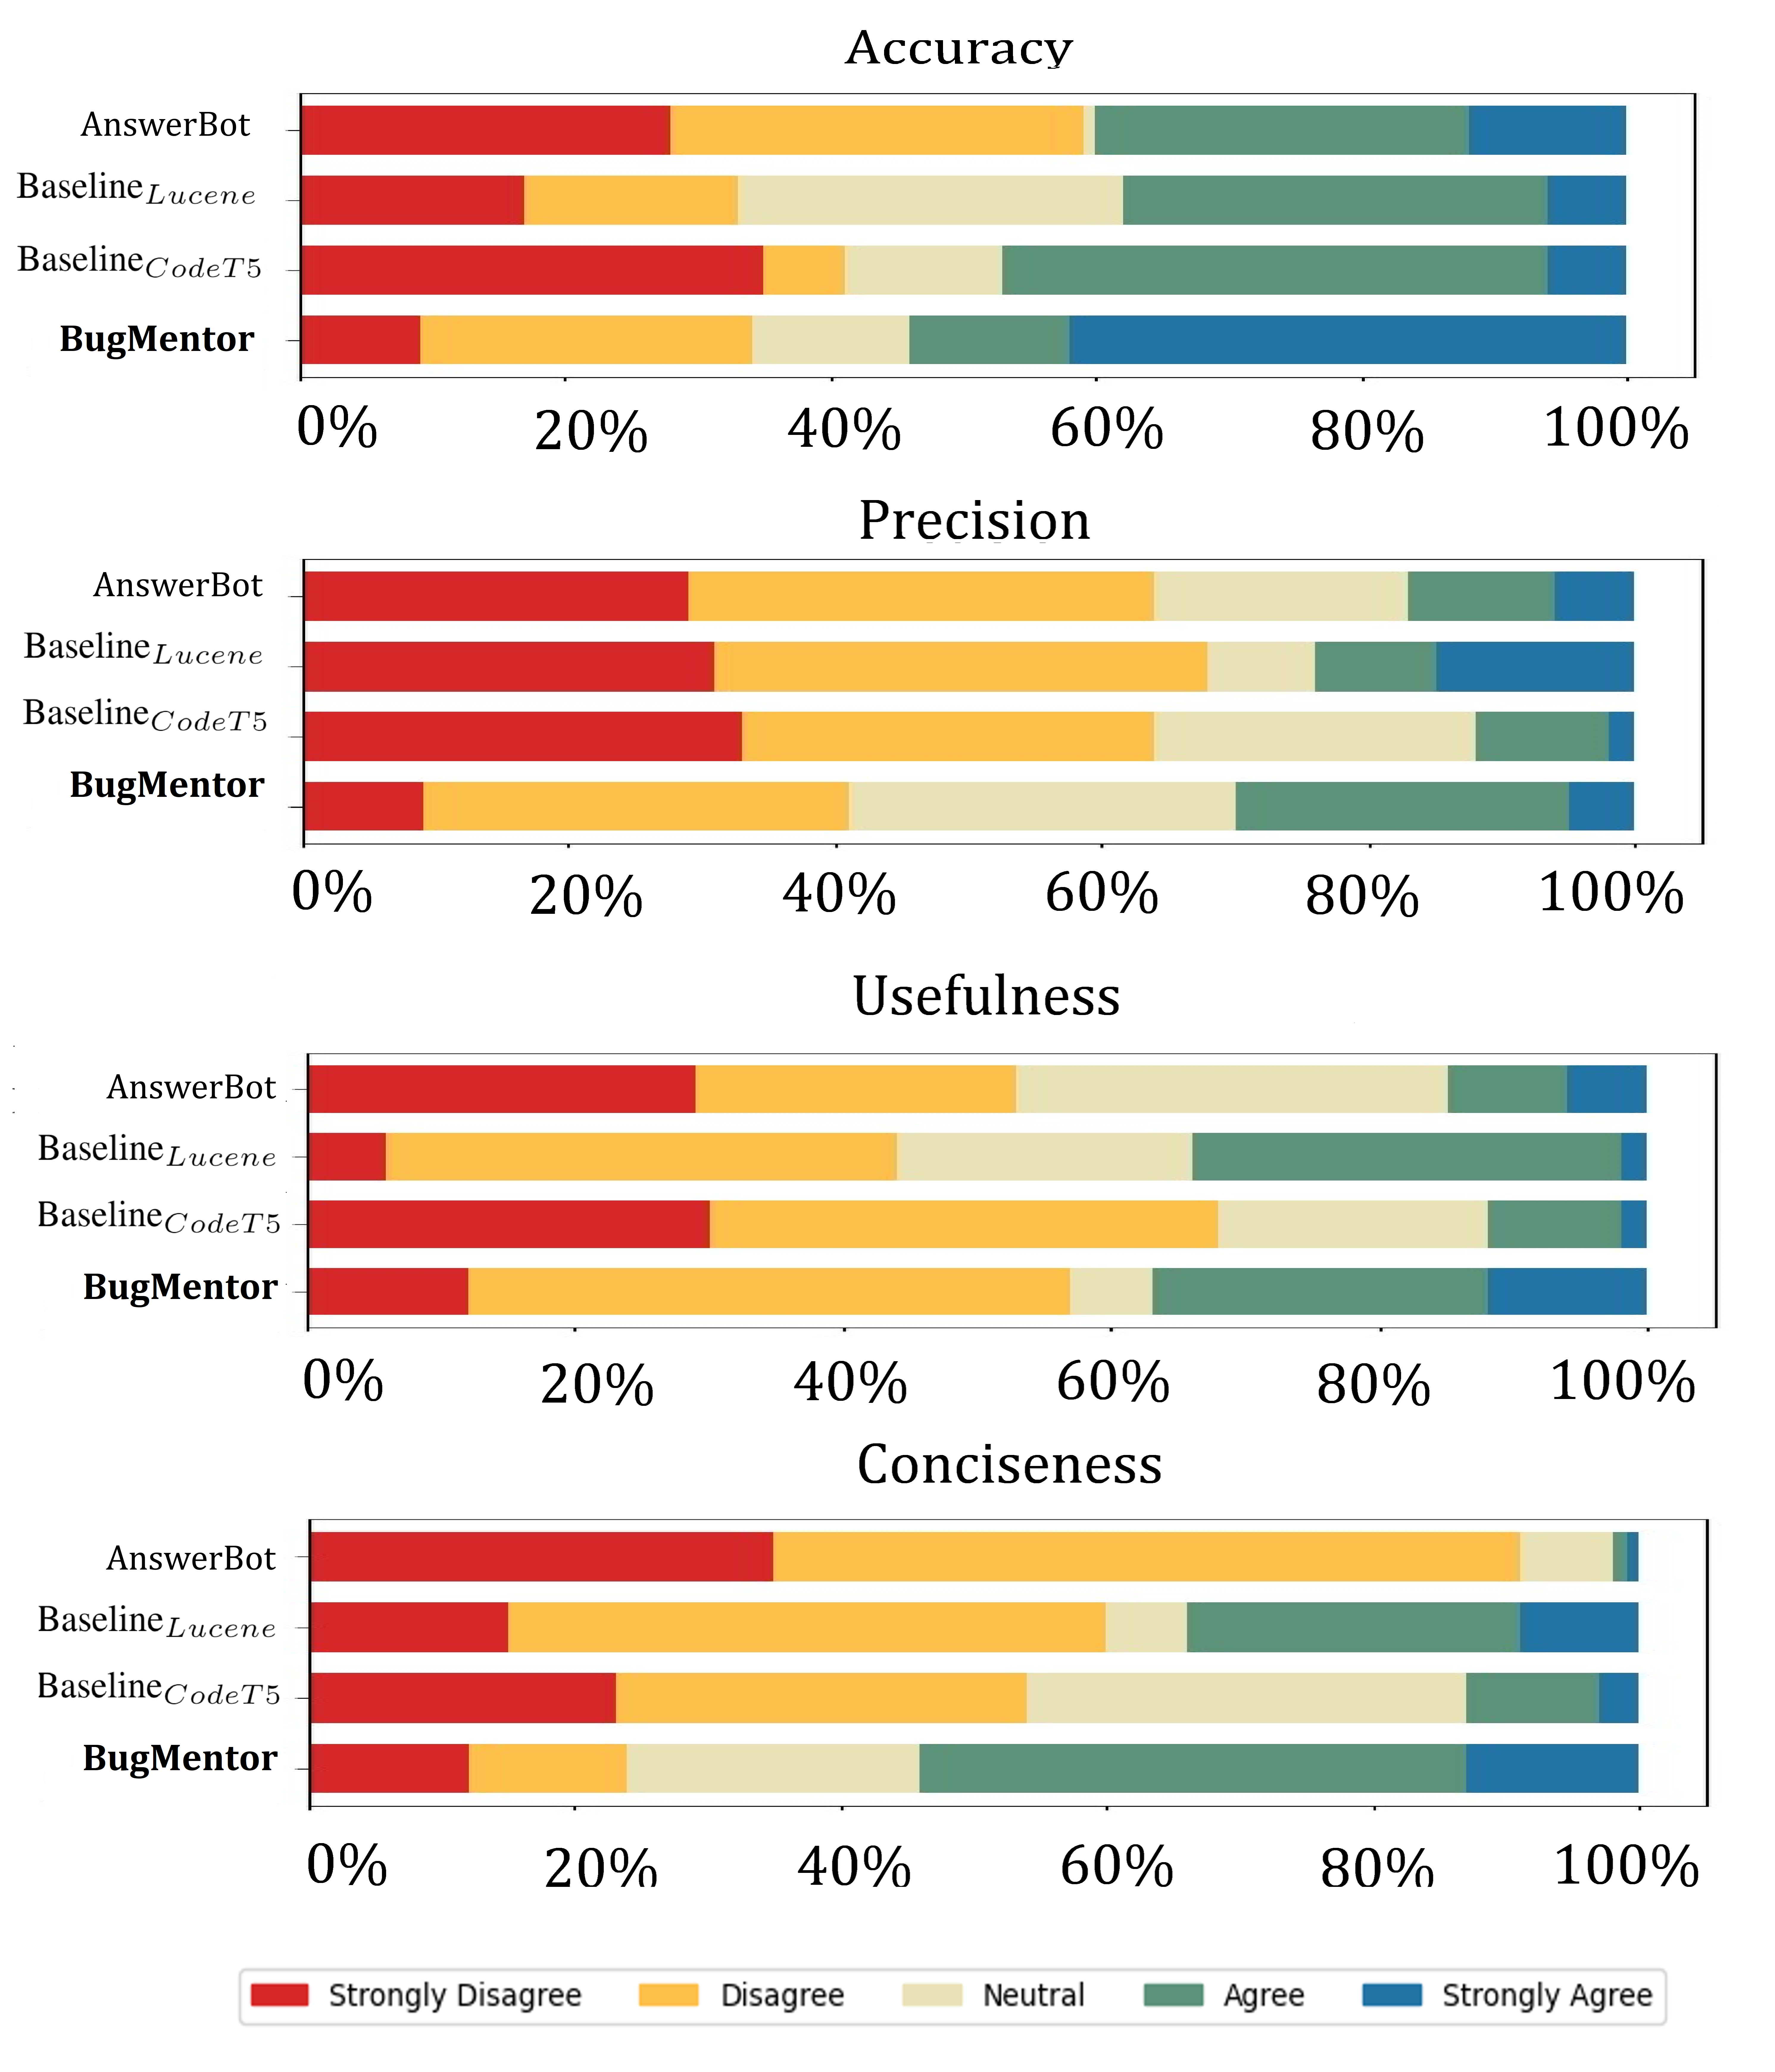
\includegraphics[width=\textwidth,keepaspectratio]{images/user_study_graph.png}
	\caption{Comparison of BugMentor with the baseline techniques using the Likert scores}
	\label{fig:dev}
\end{figure*}

\begin{table}[!ht]
\centering
\caption{Comparison of BugMentor with the Baseline Techniques using a Developer Study}
\label{tab:devstudy}
\renewcommand{\arraystretch}{1.2}
\resizebox{0.6\textwidth}{!}{
\begin{tabular}{|c|l|c|c|}
\hline
\textbf{Quality} & \multicolumn{1}{c|}{\textbf{Model}} & \textbf{Mean} & \textbf{Median} \\ \hline
\multirow{4}{*}{Accurate} & Baseline$_{Lucene}$ & 3.03 & 3 \\ \cline{2-4} 
 & Baseline$_{CodeT5}$ & 2.55 & 3 \\ \cline{2-4} 
 & AnswerBot & 2.65 & 2 \\ \cline{2-4} 
 & \textbf{BugMentor} & \textbf{3.10} & \textbf{3} \\ \hline
\multirow{4}{*}{Precise} & Baseline$_{Lucene}$ & 2.25 & 2 \\ \cline{2-4} 
 & CodeT5 & 2.56 & 3 \\ \cline{2-4} 
 & AnswerBot & 2.34 & 2 \\ \cline{2-4} 
 & \textbf{BugMentor} & \textbf{2.96} & \textbf{3} \\ \hline
\multirow{4}{*}{Useful} & Baseline$_{Lucene}$ & 2.62 & 2 \\ \cline{2-4} 
 & Baseline$_{CodeT5}$ & 2.46 & 2 \\ \cline{2-4} 
 & AnswerBot & 2.4 & 2 \\ \cline{2-4} 
 & \textbf{BugMentor} & \textbf{2.94} & \textbf{3} \\ \hline
\multirow{4}{*}{Concise} & Baseline$_{Lucene}$ & 2.68 & 2 \\ \cline{2-4} 
 & AnswerBot & 1.7 & 2 \\ \cline{2-4} 
 & Baseline$_{CodeT5}$ & 2.95 & 3 \\ \cline{2-4} 
 & \textbf{BugMentor} & \textbf{3.32} & \textbf{4} \\ \hline
\end{tabular}%
}
\end{table}

\textbf{Study Results and Discussion:} 
Table~\ref{tab:devstudy} summarizes our
findings from the developer study. We note that, on average, the participants found the answers from BugMentor to be the most accurate, precise, useful, and concise. Based on the median and mode values, we see that the participants 
agree with our answers the most.
%agree the most with answers from BugMentor. 
Similar to the findings in RQ$\mathbf{_2}$, the participants found the closest competitor of BugMentor to be Baseline$_{Lucene}$ in terms of precision, usefulness and conciseness and Baseline$_{CodeT5}$ in terms of accuracy. According to the median values, the developers agree with AnswerBot, Baseline$_{Lucene}$ and Baseline$_{CodeT5}$ in several cases. However, based on the mode values, we note that the participants disagree with their answers in many more cases.

\looseness=-1
Fig.~\ref{fig:dev} shows the distribution of participants’ agreement levels with different quality aspects of the answers. We see that the participants strongly agree with BugMentor for a substantial part of the time (e.g., $\sim$40\% for accuracy), and strongly disagree only a few times (e.g., $<$20\% times), which none of the baselines achieved. On the other hand, nearly half of the time, the participants disagree with AnswerBot, Baseline$_{Lucene}$ and Baseline$_{CodeT5}$ regarding various quality aspects of their provided answers.\par

\looseness=-1
We also perform Mann-Whitney Wilcoxon test~\cite{cuzick1985wilcoxon} to check if the developers' preferences to Baseline$_{Lucene}$, Baseline$_{CodeT5}$ and AnswerBot are significantly lower than that of BugMentor using BonFerroni Correction~\cite{weisstein2004bonferroni}. We find that the preference levels for BugMentor are significantly higher than all three baselines, i.e., p $=$ 0.0010$<$0.016 for Baseline$_{Lucene}$, p $=$ 0.0016$<$0.016 for  Baseline$_{CodeT5}$, and p $=$ 0.00016$<$0.016 for AnswerBot.

\renewcommand{\arraystretch}{1.2}
\begin{table}[htbp]
\caption{Manual Analysis}
\label{tab:manualanalysis}
\centering
\begin{threeparttable}
\begin{tabular}{|c|c|c|c|c|} \hline
\textbf{Dataset}   & \textbf{AC}    & \textbf{AP}    & \textbf{AP + AddInfo} & \textbf{AddInfo} \\ \hline \hline
Java & 7  & 9  & 12  & 20  \\ \hline
Python & 8  & 9 & 17  & 14  \\ \hline
C++  & 4 & 4 & 16  & 24 \\ \hline
JavaScript & 8  & 5  & 16  & 19  \\ \hline
\textbf{Average\%} & \textbf{14.06} & \textbf{14.06} & \textbf{31.77}        & \textbf{40.10}   \\ \hline
\end{tabular}   
\begin{tablenotes}
  \small
  \item \begin{center}
     \textbf{AC} $=$ Answers Completely, \textbf{AP} $=$ Answers Partially,\\ \textbf{AddInfo} $=$ Additional Information 
  \end{center}
\end{tablenotes}
\end{threeparttable}
\end{table}


\textbf{Manual Analysis:}
\looseness=-1
To further investigate the usefulness of BugMentor's answers, we perform a manual analysis on 192 bug reports (i.e. 48 samples for each programming language). We select these samples from the whole collection with a 95\% confidence level and 4.95\% error margin. We collect the bug reports, follow-up questions, ground truth and generated answers. Table~\ref{tab:manualanalysis} shows the summary of our analysis. \par

\looseness=-1
We analyze our generated answers to the follow-up questions, contrast them against the ground truth, and determine whether they respond to the question completely, partially or simply provide additional information. We find that BugMentor, on average, was able to answer the questions completely for 14.06\% of the cases from each programming language. It was able to answer 14.06\% of the questions partially while adding complementary information to 31.77\% of the answers. Furthermore, in 40\% cases, our technique delivered such answers that did not match with the ground truth answers but were complementary or somewhat relevant to the questions. For example, let us consider the bug report shown below discussing the issue of links in Atom. It does not provide the version of the operating system that the reporter uses. The ground truth answer indicates the OS version and the issue persistence in the safe mode of the browser. We see that BugMentor's answer captures the context and points out that the problem might lie with Ubuntu version rather than other running applications. Thus, BugMentor can provide complementary information that can benefit the developer.


\begin{frshaded}
\noindent
\textbf{Title:} Links do not work in Atom \\
\textbf{Description:} After upgrading to Atom, links no longer open in a new tab in Chrome. For example, clicking on any of the release notes links does nothing. \\
\textbf{Question:} What OS do you experience this issue in safe mode? \\
\textbf{Actual Answer:} Ubuntu; safe mode exhibits the same issue. \\
\textbf{Generated Answer:} Since upgrading to Ubuntu, I've had no issues. However, similar problems with other apps make me suspect it's related to the Ubuntu version. Even in safe mode, Atom still exhibits the problem.
\end{frshaded}

\FrameSep.3em
\begin{frshaded}
	\noindent
        \looseness=-1
	\textbf{Summary of RQ$\mathbf{_4}$:} Developers with professional experience found the answers of BugMentor to be accurate, precise, concise, and useful, with respect to the ground truth answers. Their preference levels for BugMentor were also higher than those of the three baseline techniques by a statistically significant margin.  
\end{frshaded}


\section{Related Work} \label{Chap1:RelatedWork}

\looseness=-1
Question Answering (QA) has been an active research topic in both Information Retrieval (IR) and Natural Language Processing (NLP) communities~\cite{ravichandran2002learning, brill2002analysis,waltz1978english, iyyer2014neural,asaduzzaman2013answering, tian2017apibot, lu2021beat, bansal2021neural, xu2017answerbot, abdellatif2020msrbot}. There also have been several works that focus on question-answering in the context of software engineering. Breu et al.~\cite{breu2010information} first analyzed follow-up questions from bug reports and found that 32.34\% of them were never responded to. Recently, Imran et al.~\cite{imran2021automatically} proposed Bug-AutoQ that recommends follow-up questions against a deficient bug report leveraging development history using information retrieval. However, their technique does not answer the follow-up questions.\par


\looseness=-1
Murgia et al.~\cite{murgia2016among} leverage the search feature of StackOverflow Q\&A site to suggest relevant questions against error messages from a version control system. However, their technique was trained to provide only simple, recurring questions related to Git error messages. Tian et al.~\cite{tian2017apibot} propose APIBot that can answer questions related to an API by analyzing the relevant API documentation. However, their solution was limited to API-related questions only. Bansal et al.~\cite{bansal2021neural} design a context-aware QA system to answer basic questions about subroutines. Lu et al.~\cite{lu2021beat} propose another QA approach that can provide answers by executing structured queries generated from a bug report template. Xu et al.~\cite{xu2017answerbot} designed AnswerBot to synthesize answers for technical, non-factoid questions from StackOverflow. 
However, they only use the title of a question overlooking the detailed problem context (e.g., question body), and thus their answers might be unaware of the problem context. We compare BugMentor with AnswerBot using experiments, and the detailed comparison can be found in Section~\ref{results:rq2}. Abdellatif et al. ~\cite{abdellatif2020msrbot} designed MSRBot to answer the most common questions related to software development and maintenance. However, their answers might be limited by the available information in the mined repositories. Song et al.~\cite{song2022toward} designed BURT to support bug reporters of Android applications, but their approach might not generalize to other software applications.

Recently, Language Model-based approaches (LLMs) such as ChatGPT have emerged as a powerful text generation tool. After conducting a limited qualitative analysis (Section~\ref{results:rq2}), we note that while ChatGPT exhibit an understanding of a given bug report, they often struggle to come up with precise answers to follow-up questions. BugMentor has a better understanding of past bug reports and thus captures a broader context. In the future, we plan on conducting a thorough comparison between BugMentor and contemporary LLM-based approaches like ChatGPT.


In short, existing relevant works focus on improving deficient bug reports and answering specific questions related to API, subroutines and Git error messages. 
To the best of our knowledge, our proposed technique is the first to automatically answer the follow-up questions from bug reports, which makes our work \emph{novel}. We also combine structured information retrieval with neural text generation (e.g., CodeT5) to generate the answers, which were found to be meaningful, accurate, precise, useful, and concise according to two types of evaluation --- automated metrics and developer study. Our technique also outperforms three baselines.  


\section{Threats to Validity} \label{Chap1:Threats}
We identify a few threats to the validity of our findings. In this section, we examine these threats and discuss the steps that were taken to mitigate them.\par

\looseness=-1
\textbf{External Validity:}
Threats to external validity refer to the lack of generalizability in the findings~\cite{ferguson2004external}. One threat could stem from our selection of subject systems. We select 20 software systems written in four programming languages: Python, Java, JavaScript, and C++, which might not represent all systems at GitHub. However, the underlying algorithm of BugMentor is not bound to any programming language and thus can be easily adapted to any other platforms.\par
Another threat stems from the small sample size of the held-out dataset for evaluation (e.g., 550). However, to mitigate this concern, we selected them carefully through random sampling from all four subsets (95\% confidence level, 4.06\% error margin, Section~\ref{sec:groundtruth}). We also maintain diversity in selecting our 20 subject systems (Section~\ref{sec:groundtruth}). 

\looseness=-1
\textbf{Construct Validity:} Construct validity refers to the extent to which the experiment measures what it intends to measure~\cite{smith2005construct}. 
Inappropriate use of evaluation metrics could be a threat to construct validity. However, we chose our evaluation metrics --- BLEU, METEOR, Semantic Similarity, and WMD --- based on relevant literature~\cite{papineni2002bleu,banerjee2005meteor,haque2022semantic,huang2016supervised}. We also chose the four quality aspects of generated answers based on relevant literature~\cite{imran2021automatically,joshi2015likert}. Thus, threats to construct validity might be mitigated.

\looseness=-1
\textbf{Internal Validity:} Threats to internal validity relate to experimental errors and subjective biases~\cite{christ2007experimental}. We use manually annotated ground truth to answer both RQ1 and RQ2, which could be a source of threat. However, to mitigate this, the annotators were given appropriate training for their annotation tasks. We also employ majority voting~\cite{kuhrmann2017pragmatic} for decision-making and calculate Cohen's $\kappa$ to demonstrate the agreement levels between annotators~\cite{kuhrmann2017pragmatic}.
In the developer study, the assessment of answers can be influenced by subjective bias. However, we anonymize the source of all answers to avoid any bias towards any technique.
\looseness=-1
Another source of threat could be the replication of the baseline techniques. For the replication of CodeT5, we collected the pre-trained model from HuggingFace~\cite{huggingface_t5}, and for the replication of Lucene, we used ElasticSearch~\cite{ElasticSearch}, a standard library. To replicate AnswerBot~\cite{xu2017answerbot}, we used the replication package from the original authors~\cite{maxxbw54}. Furthermore, we followed the documentation closely for any customizations. Thus, threats to internal validity might be mitigated.
 
\section{Summary} \label{Chap1:Summary}

To summarize, in this study, we propose BugMentor, a novel technique to answer follow-up questions from deficient bug reports by combining structured information retrieval and neural text generation. Our technique leverages the relevance between past and current bug reports to gather additional context, which helps us generate an appropriate answer to the question. Our evaluation using four performance metrics shows that BugMentor can generate understandable and good answers to follow-up questions, as per Google's Standard. Our technique outperforms three existing baselines. We also evaluate BugMentor using a user study using 10 developers. The developers found the answers from BugMentor to be more accurate, precise, concise and useful compared to the baseline answers. Thus, BugMentor has the potential to support bug resolution with complementary information in the form of answers to follow-up questions. However, newcomers or novice developers often struggle to understand bug reports due to their lack of in-depth knowledge about an application. Thus we perform another study to further improve the quality of bug reports by providing explanations to their domain-specific terms or jargon.

\chapter{BugEnricher: Explaining Domain-specific Terms and Jargon from Bug Reports with Neural Machine Translation} \label{Chap2:BugEnricher}

\looseness=-1
Existing studies have shown that about 78\% of bug reports from open-source projects (e.g., Eclipse, Firefox) include less than 100 words each and claim more time from developers for bug resolution~\cite{zhang2017bug}. Our first study in Chapter \ref{chapter:BugMentor} aims to support the developers by generating answers to follow-up questions from deficient bug reports. While our answers have been found useful, novice developers might need more help in their bug understanding. In this chapter, we propose --- \textit{BugEnricher} --- that can supplement bug reports with meaningful explanations to their domain-specific terms or jargon. Our evaluation using three performance metrics (e.g., BLEU, METEOR, Semantic Similarity) shows that \textit{BugEnricher} can generate understandable and good explanations according to Google’s standard and can outperform existing baselines from the literature. \par

The rest of this chapter is organized as follows. Section~\ref{Chap2:Intro} introduces our study and reports the gap in the literature and our contribution. Section~\ref{Chap2:Motivation} illustrates the usefulness of our technique with a motivating example. Section~\ref{Chap2:Methodology} presents our proposed technique for explaining software-related terms. Section~\ref{Chap2:ExperimentalSetup} discusses our experimental design and datasets.
Section~\ref{Chap2:Results} discusses our evaluation results. Section~\ref{Chap2:RelatedWork} discusses relevant studies from the literature. Section~\ref{Chap2:Threats} identifies possible threats to the validity of our work. Finally, Section~\ref{Chap2:Summary} summarizes this study.


\section{Introduction} \label{Chap2:Intro}

Software bugs are human-made mistakes that prevent a software system from operating as expected.
According to a recent study~\cite{britton2013reversible, zou2018practitioners}, software bugs cause the global economy to suffer enormously and lose billions of dollars every year. Bug finding and corrections take up approximately 50\% of a developer's programming time. Bug resolution is, therefore, one of the most challenging issues in software maintenance~\cite{zou2018practitioners}. Hundreds of software bugs are submitted as \textit{bug reports} to bug-tracking systems such as GitHub and JIRA~\cite{anvik2006should}. The developers then examine and resolve these bugs by carefully analyzing the corresponding bug reports.

% motivation
Given a reported bug, developers need to first understand its root cause and symptom before they come up with a solution~\cite{bohme2017directed}. A recent study suggests that information in the majority of bug reports is incomplete and inaccurate~\cite{davies2014s,bugde2008global}. Zhang et al.~\cite{zhang2017bug} found that up to 78\% of bug reports from four open-source projects (e.g., Eclipse, Mozilla, Firefox, GCC) contain less than 100 words each (a.k.a., short bug reports). These short bug reports, on average, took 121 extra days to get resolved when compared to the well-written bug reports due to the lack of information~\cite{zhang2017bug}. Thus, understanding the bug reports could be a challenge due to incomplete or inaccurate information with complex problem context~\cite{velly2013towards}. This challenge could exacerbate for newcomers or novice developers to a project who need additional assistance to understand or resolve a bug. According to a recent study~\cite{guizani2021long}, even with prior experience, developers often need help to acquire a comprehensive understanding of any application domain and understand the discussions from a bug report. One significant obstacle to bug understanding for novice developers could be the lack of explanation for the domain-specific terms or jargon in the bug reports.\par

% why existing work is not sufficient
\looseness=-1
There have been existing studies to support newcomers or inexperienced developers who may struggle to comprehend the bug reports. An existing survey by Tan et al.~\cite{tan2020first} found that a clear bug description, which does not rely on in-depth domain knowledge, is crucial to assist newcomers in understanding and resolving the bug. Recently, Correa et al.~\cite{correa2013samekana} suggest that including web links in issue tracker discussions can benefit developers by providing external knowledge sources or artifacts. Zhang et al.~\cite{zhang2017bug} recommend complementing bug reports with carefully curated sentences from relevant past bug reports. Dit et al.~\cite{dit2008improving} propose a technique that suggests relevant comments from past bug reports so that developers can make explicit connections between the suggested and existing comments. Including such comments in a bug report can be helpful for the developers to gain a better understanding of the issue. While the above approaches offer complementary information to support bug understanding, they do not focus on domain-specific terms or jargon, which warrants further investigation.\par

% approach
\looseness=-1
In this chapter, we propose a novel technique --- BugEnricher --- that can supplement bug reports by generating explanations for their domain-specific terms and jargon using neural text generation. First,  we construct a vocabulary for two popular programming languages --- Java and Python. We scrape the domain-specific terms or jargon and their explanations from three different sources --- StackOverflow, Glossary, and API documentation. Second, we fine-tune a transformer-based text-generation model (e.g., T5) with the domain-specific terms or jargon and their corresponding explanations collected above. Third, we generate the explanations for domain-specific terms from bug reports using our fine-tuned model and examine their effectiveness using a case study.\par

\looseness=-1
We collect 28,7690 Java, 21,365 Python and 141,567 miscellaneous domain-specific terms or jargon and their explanations from the aforementioned sources for our experiments. We evaluate our technique --- BugEnricher --- using three popular metrics on text generation, namely BLEU score~\cite{papineni2002bleu}, METEOR~\cite{banerjee2005meteor}, Semantic Similarity Score~\cite{haque2022semantic}. We achieve a BLEU score of 28.85, which is understandable to good according to Google AutoML documentation~\cite{automldoc}. Our technique also outperforms two baselines --- AnswerBot~\cite{xu2017answerbot} and T5~\cite{raffel2020exploring} --- in all three metrics. We also conduct a case study using duplicate bug reports and attempt to enrich duplicate bug reports that are textually dissimilar~\cite{jahan2023towards}. We find that the enrichment of bug reports by BugEnricher led to an improvement in the performance of an existing technique for duplicate bug detection. Thus, the empirical findings above suggest that our technique has the potential to enrich a bug report significantly, which could lead to improved bug understanding and management.

% summary
We thus make the following contributions in this study:
\begin{enumerate}
    \item[(a)] A large dataset of 141,567 domain-specific terms and jargon and their corresponding explanations that are carefully curated from Stack Overflow Q\&A site, glossary, and API documentation.
    \item[(b)] A novel approach --- BugEnricher --- that can complement bug reports with meaningful explanations of their domain-specific terms or jargon using neural text generation (e.g., fine-tuned T5).
    \item[(c)] A replication package~\cite{bugenricherreplicationpackage} that includes our working prototype, experimental dataset, and other configuration details for the replication or third-party reuse.
\end{enumerate}    



\section{Motivating Example} \label{Chap2:Motivation}
% url  : https://bugs.eclipse.org/bugs/show_bug.cgi?id=440607
%  url : https://bugs.eclipse.org/bugs/show_bug.cgi?id=497389
\begin{figure}[!htpb]
  \centering
  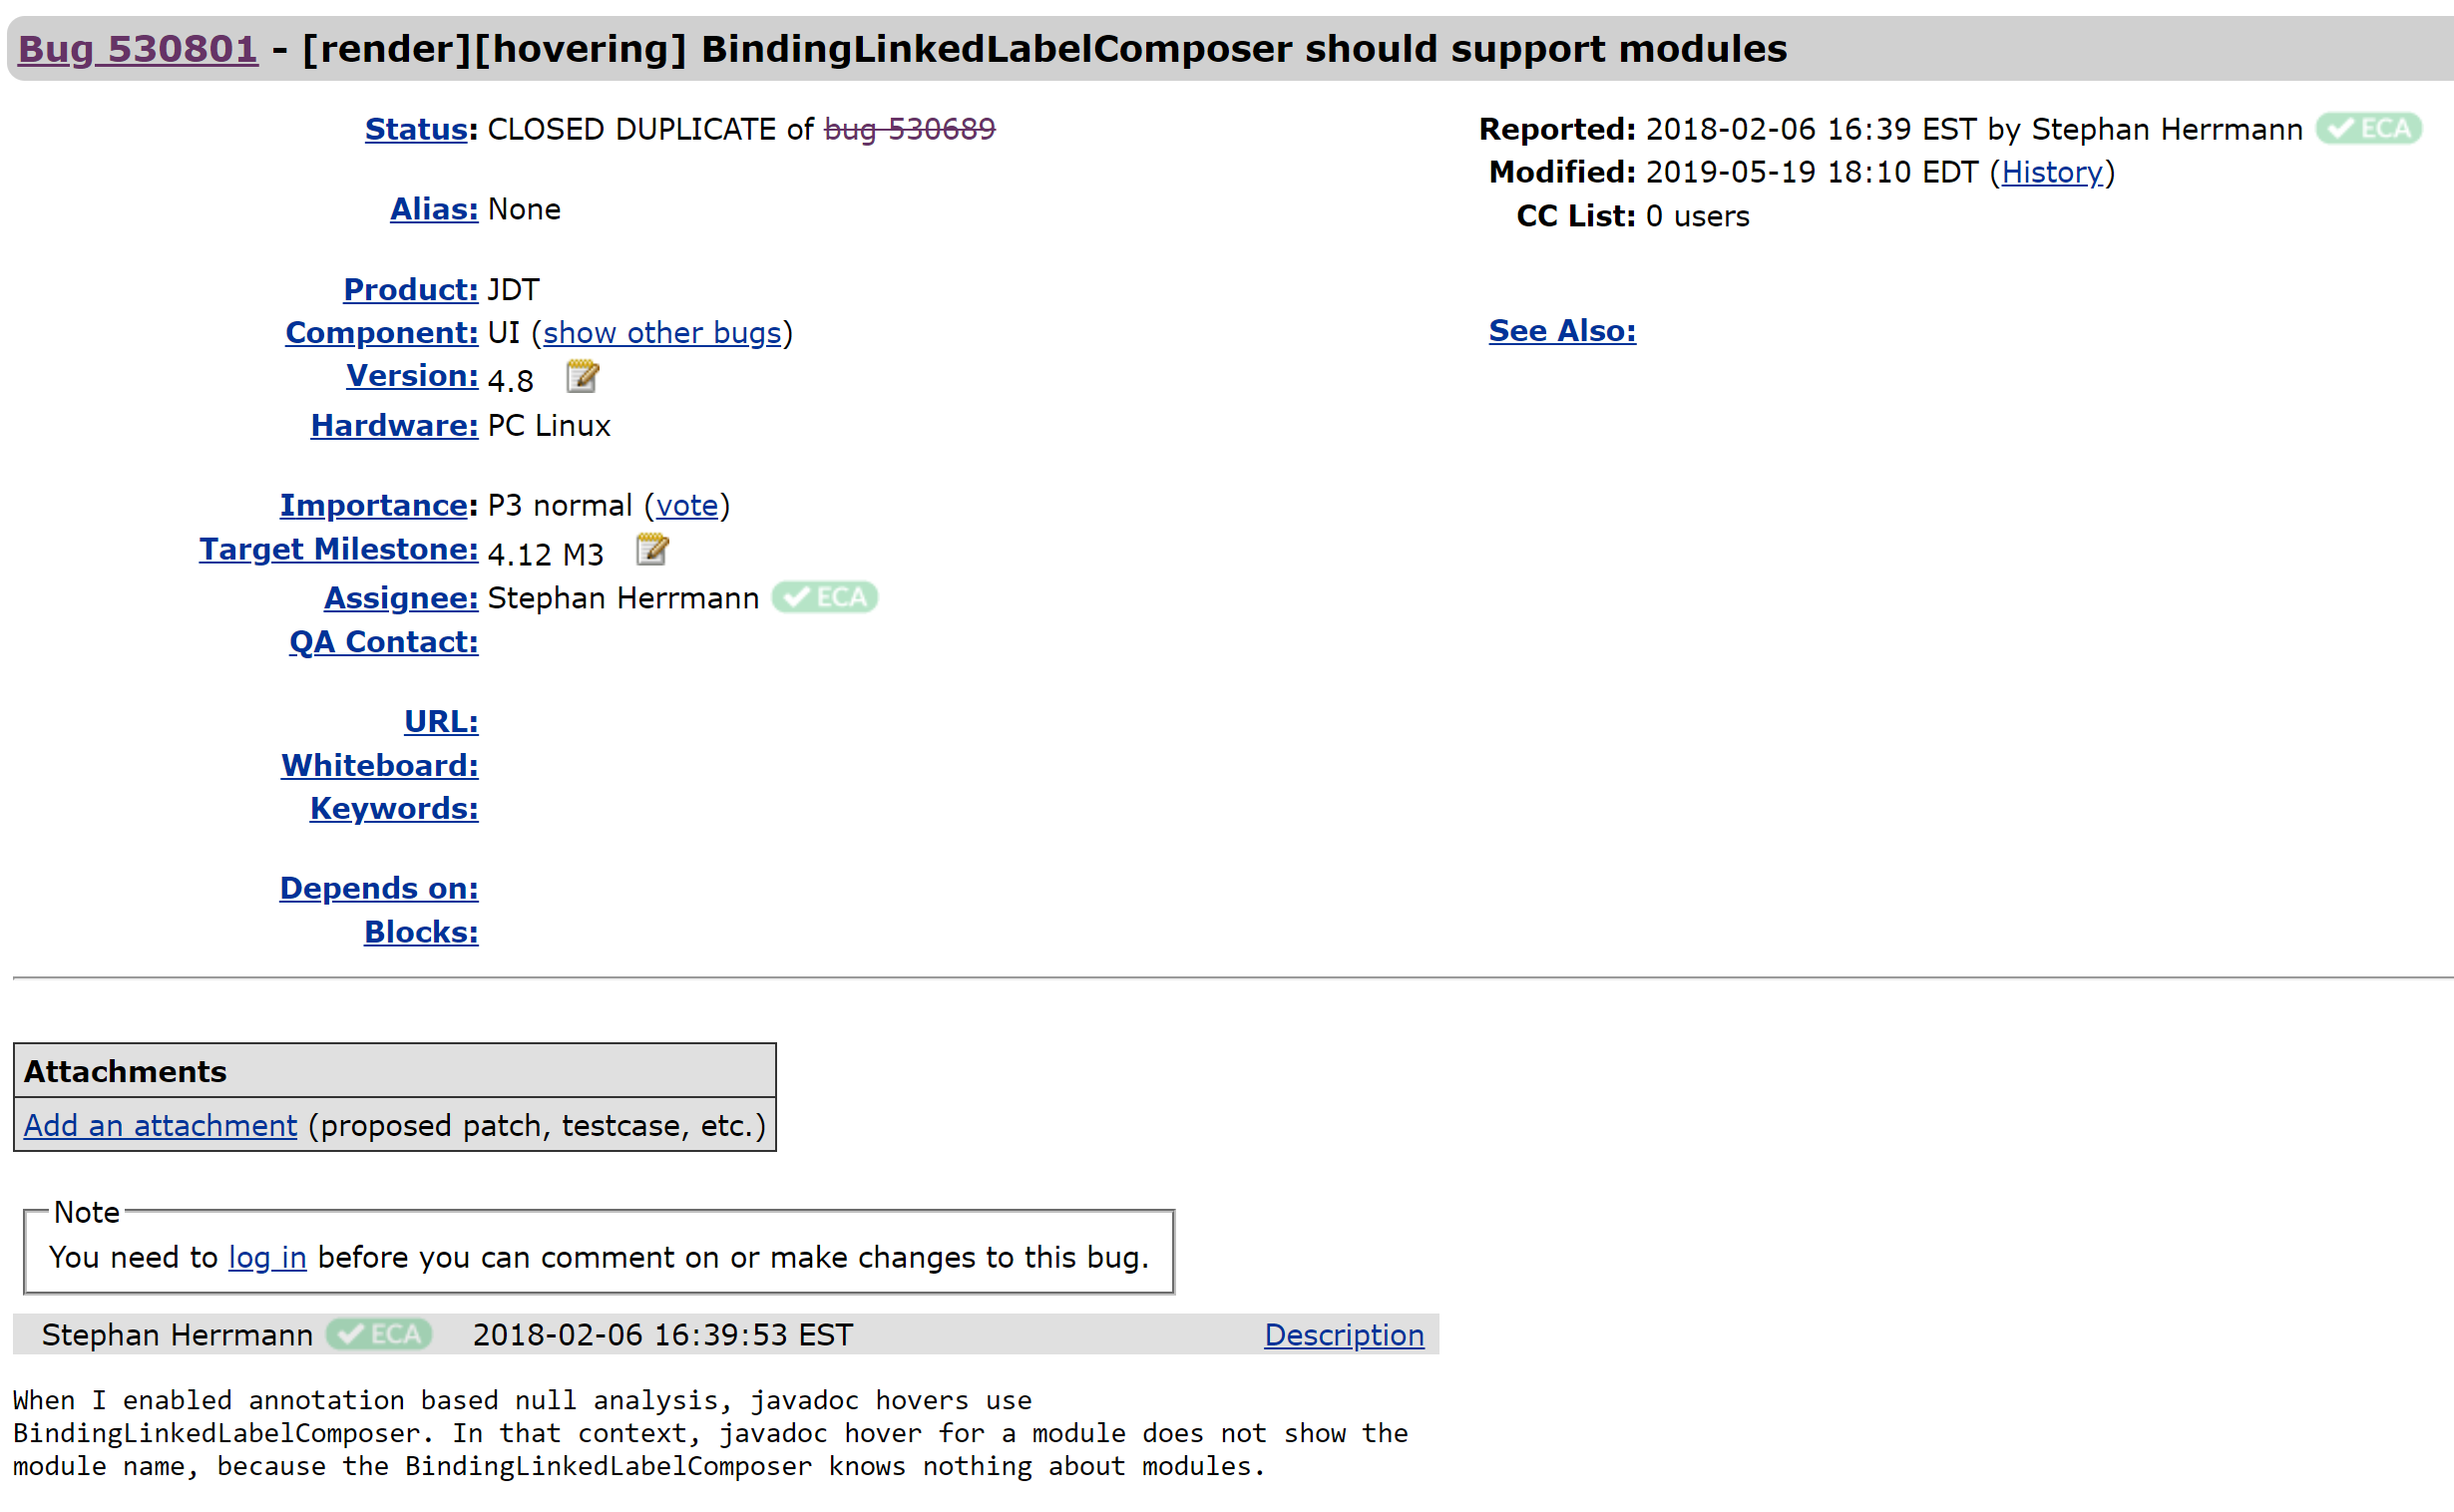
\includegraphics[width=0.9\textwidth]{images/motivatingexampleBE.png}
  \caption{An example of a bug report from BugZilla (ID \#530801)}
  \label{Chap2_fig:motivating_example}
\end{figure}

\begin{table}[!ht]
\centering
\caption{Generated Explanations by BugEnricher}
\label{BugEnricherGeneratedExplanations}
\resizebox{\textwidth}{!}{%
\begin{tabular}{|l|l|}
\hline
\textbf{Domain-Specific Terms or Jargon} & \textbf{Explanations} \\ \hline
Javadoc & It is documentation generated  \\ \hline
BindingLinkedLabelComposer & It is for composing labels \\ \hline
annotation & It is used to describe an annotation object \\ \hline
null-analysis & It is a Java library for analyzing null data \\ \hline
module & It is a unit of Java code \\ \hline
\end{tabular}%
}
\end{table}

\looseness=-1
To demonstrate the potential benefits of our work, let us consider the example bug report in Fig.~\ref{Chap2_fig:motivating_example}. It has been taken from the \emph{Eclipse} project on BugZilla\footnote{\url{https://bugs.eclipse.org/bugs/show_bug.cgi?id=530801}\label{chap2_motivating_example}}. The example report discusses a bug related to BindingLinkedLabelComposer that lacks awareness of modules. The problem stems from Javadoc when using the annotation-based null analysis. Specifically, the module name does not appear when hovering over a module. Table~\ref{BugEnricherGeneratedExplanations} shows the explanations generated by BugEnricher. These explanations were used to enrich the example bug report, and the enriched bug report can be found below.\par

\FrameSep.2em
\begin{frshaded}
\label{enrichedbugreport}
\noindent
 \textbf{Enriched Bug Report} \\
 \looseness=-1
When I enabled annotation (It is used to describe an annotation object) based null analysis (It is a Java library for analyzing null data), Javadoc (It is documentation generated) hovers use BindingLinkedLabelComposer (It is for composing labels). In that context, Javadoc hover for a module (It is a unit of Java code) does not show the module name, because the BindingLinkedLabelComposer knows nothing about modules.
\end{frshaded}

In our case study, the enriched bug report improved the rank of its duplicate report from the 19th to the 13th position in the ranked list when detected by a BM25-based technique~\cite{yang2012duplication,jahan2023towards}. This significant improvement in the ranking highlights the importance of our provided explanations, demonstrating an improvement in the quality of bug reports.

\section{Methodology} \label{Chap2:Methodology}

As input, our technique takes a bug report containing domain-specific terms or jargon that require additional explanation. As output, it generates explanations for those terms. Fig.~\ref{Chap2_fig:schematic} shows the schematic diagram of our proposed technique. In the following sections, we discuss different steps of our approach.\par 

\begin{figure}[!t]
  \centering
  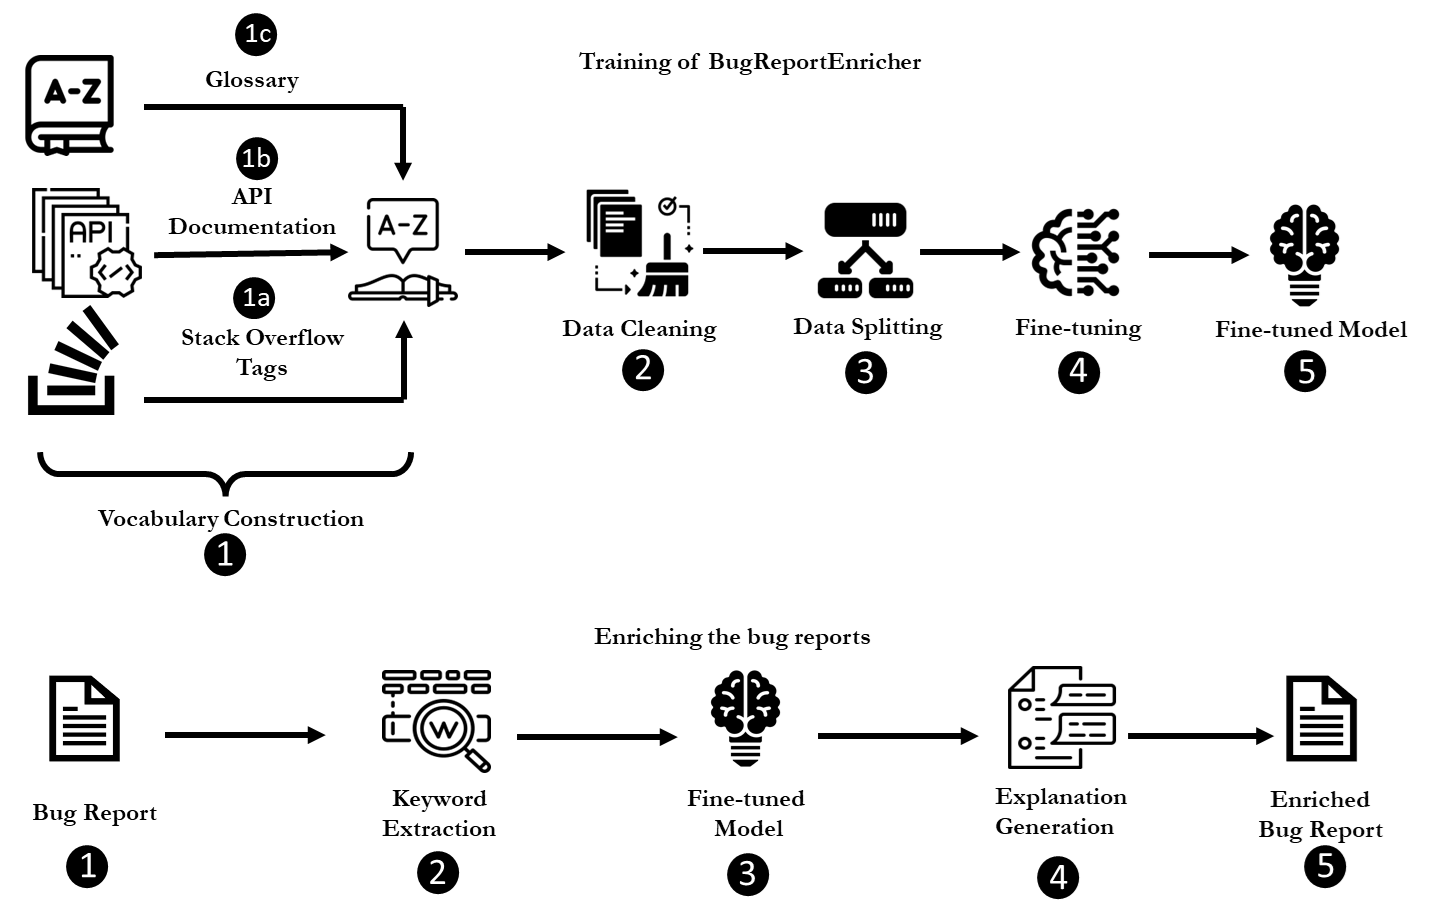
\includegraphics[ width=\textwidth, height=7.5in, keepaspectratio]{images/BugRepEnricherSchematic.png}
  \caption{Schematic diagram of BugEnricher}
  \label{Chap2_fig:schematic}
\end{figure}

\subsection{Vocabulary Construction}
First, we construct a vocabulary of domain-specific terms along with their meanings (a.k.a., explanations) for two popular programming languages --- Python and Java. We collect them from three different sources --- StackOverflow Tags, API Documentation and Glossary.

\subsubsection{(a) StackOverflow Tags}
To collect the domain-specific terms and their meanings, we use StackOverflow as our first source. Each post on StackOverflow consists of several tags that convey the key concepts of the post. The meaning of each tag is defined on StackOverflow. We collect 10,022 Java tags, 9,594 Python tags and 105,822 miscellaneous tags from \acrfull{sede} using the SQL query --- ``select $*$ TagName from Tags". The ``Tags" table contains all the name of the tags in the ``TagName" field. To capture the Java or Python related tags, we collect a list of Tags that contain the keyword ``Java" and ``Python" or "py" in their names. We then scrape the explanations of all the collected Tag names using Beautiful Soup\footnote{\url{https://pypi.org/project/beautifulsoup4/}}. An example of the StackOverflow tag is shown below.\par

\FrameSep.2em
\begin{frshaded}
\label{sotag}
\noindent
\textbf{Tag and Explanation at StackOverflow}\\
\textbf{Tag}: google-chrome-extension \\
\textbf{Explanation}: Extension development for the Google Chrome web browser. You write them using web technologies such as HTML, JavaScript, and CSS.
\end{frshaded}

\FrameSep.2em
\begin{frshaded}
\label{sotag2}
\noindent
\textbf{Java related Tag and Explanation at StackOverflow}\\
\textbf{Tag}: javafx-11 \\
\textbf{Explanation}: The JavaFX platform enables developers to create client applications based on JavaSE that behave consistently across multiple platforms. Built on Java technology since JavaFX 2.0, it was part of the default JDK since JDK 1.8, but starting Java 11, JavaFX is offered as a component separate from the core JDK.
\end{frshaded}

\FrameSep.2em
\begin{frshaded}
\label{sotag3}
\noindent
\textbf{Python related Tag and Explanation at StackOverflow}\\
\textbf{Tag}: python-mode \\
\looseness=-1
\textbf{Explanation}: Python-mode is a vim plugin that helps you to create Python code very quickly by utilizing libraries including pylint, rope, pydoc, pyflakes, pep8, and mccabe for features like static analysis, refactoring, folding, completion, documentation, and more.
\end{frshaded}

\looseness=-1
\subsubsection{(b) API Documentation}
We collect the API documentation of the most recent stable version of both Python (3.11) and Java (17) programming languages from their official documentation~\cite{pythonDocumentation,javaDocumentation}. We use Beautiful Soup\footnote{\url{https://pypi.org/project/beautifulsoup4/}} and Request\footnote{\url{https://pypi.org/project/requests/}} libraries for all our scraping.\par
First, we scrape the overview page from the official documentation containing the names of all the modules, their explanations and the URLs to further description of the defined packages and services. We store these module names and their explanations. Then, from the URLs collected in the previous step, we further scrape the package and service names, their explanations, and the URLs to further description of the defined classes and interfaces. Similarly, from the URLs collected in the previous step, we collect the classes and interfaces names, their explanations, and the URLs to the fields, methods and constructors names and their explanations. In total, we collect 18,738 Java and 11,771 Python terms and their explanations from the API documentation. An example of the terms and corresponding explanations from Java 17 and Python 3.11 API documentation is shown below.\par 

\FrameSep.2em
\begin{frshaded}
\label{apitagjava}
\noindent
\textbf{Term and Explanation from Java 17 API Documentation}\\
\textbf{java.io:} Provides for system input and output through data streams,
 serialization and the file system.\\
\textbf{java.lang:} Provides classes that are fundamental to the design of the Java
 programming language.
 \end{frshaded}

\FrameSep.2em
\begin{frshaded}
\label{apitagpython}
\noindent
\textbf{Term and Explanation from Python 3.11 API Documentation}\\
\textbf{str.splitlines:} Return a copy of the string with the leading and trailing characters removed.\\
\textbf{int.bit$\_$count:} Return the number of ones in the binary representation of the absolute value of the integer. This is also known as the population count.
 \end{frshaded}

\subsubsection{(c) Glossary}
As our third source, we collect 126 Java and 244 Python language-specific terms defined in the glossary. For Java we scrape from the oracle glossary \footnote{\url{https://www.oracle.com/java/technologies/glossary.html}\label{java-glossary}} and for python we scrape from the python glossary\footnote{\url{https://docs.python.org/3.11/glossary.html}\label{python-glossary}}.\par 
\FrameSep.2em
\begin{frshaded}
\label{glossarytag}
\noindent
\textbf{Term and Explanation from Java and Python Glossary}\\
\textbf{Python:} \\
\textbf{DOM:} Document Object Model. A tree of objects with interfaces for traversing the tree and writing an XML version of it, as defined by the W3C specification.\\
\textbf{Java:} \\ 
\textbf{immutable:} An object with a fixed value. Immutable objects include numbers, strings and tuples. Such an object cannot be altered.  A new object has to be created if a different value has to be stored.  They play an important role in places where a constant hash value is needed, for example, as a key in a dictionary.
 \end{frshaded}

After collecting the data from the three data sources, we discard any duplicates based on their terms and explanations. We divide the data into three different subsets --- Java, Python and Miscellaneous. The miscellaneous subset consists of terms and explanations from different programming languages. Table~\ref{tab:dataset} contains the descriptive statistics of our dataset. We find that the average length of each domain-specific term is approximately 13 characters, and their explanations have an average length of approximately 188 characters. \par

\renewcommand{\arraystretch}{1.4}
\begin{table}[htbp]
\centering
% \begin{threeparttable}
\caption{Dataset Details}
\label{tab:dataset}
\resizebox{\textwidth}{!}{%
\begin{tabular}{|c|c|c|c|c|c|}
    \hline
    \textbf{PL} & \textbf{Source} & \textbf{Size} & \begin{tabular}[c]{@{}c@{}}\textbf{ATL}\\ \textbf{(characters)}\end{tabular} & \begin{tabular}[c]{@{}c@{}}\textbf{AEL}\\ \textbf{(characters)}\end{tabular} & \textbf{Complete Size} \\ \hline \hline
    \multirow{3}{*}{Python} & Stack Overflow & 10,022 & 10.58 & 115.27 & \multirow{3}{*}{28,760} \\ \cline{2-5}
     & API Documentation & 18,738 & 16.72 & 360.10 &  \\ \cline{2-5}
     & Glossary & 126 & 14.31 & 361.40 &  \\ \hline
    \multirow{3}{*}{Java} & Stack Overflow & 9,594 & 11.88 & 121.38 & \multirow{3}{*}{21,365} \\ \cline{2-5}
     & API Documentation & 11,771 & 15.90 & 89.61 &  \\ \cline{2-5}
     & Glossary & 244 & 10.87 & 154.19 &  \\ \hline
    Micellaneous & Stack Overflow & 105,822 & 11.55 & 114.02 & 105,822 \\ \hline
    \end{tabular}
    }
    \vspace{-0.1cm}
\begin{threeparttable}
\begin{tablenotes}[flushleft]
  \small
  \item \begin{center}
      \item \textbf{PL} $=$ Programming Language, \textbf{ATL} $=$ Average Term Length,
      \item \textbf{AEL} $=$ Average Explanation Length
  \end{center} 
\end{tablenotes}
\end{threeparttable}
\end{table}

\subsection{Data Cleaning}
We use standard natural language pre-processing techniques to clean the domain-specific terms or jargon and their explanations. First, we remove the noisy elements like --- HTML tags and URLs. Second, we use the \textit{``pyspellchecker''}, a spell-checking library\footnote{\url{https://pypi.org/project/pyspellchecker/}\label{spellchecker}} to correct the spellings of any misspelled words. We then perform lemmatization on all items in our corpus. This step ensures that words are transformed into their root forms, facilitating better analysis~\cite{pramana2022systematic}.\par

\subsection{Data Splitting}
\label{Chap2:Methodology_datasplitting}

After we obtain the cleaned data from the previous step, we split each subset of terms and explanations into training, validation and test sets. We split each subset of our dataset (Java, Python, Miscellaneous) into training, validation and testing with the following ratios: 80\% training, 10\% validation, and 10\% testing data.

\subsection{Fine Tuning the Model}
\looseness=-1
\textbf{Model Input, Output and Structures:} 
We fine-tune the T5 model from HuggingFace\footnote{\url{https://huggingface.co/t5-base}} on the T5ForConditionalGeneration variant~\cite{huggingface_t5}, with our collected data. We use domain-specific terms or jargon as input (a.k.a., source sentence) and their explanations as output (a.k.a., target sentence). We train the T5 model with its associated encoder and tokenizer~\cite{raffel2020exploring}. The model has a 512-dimensional embedding size, a 6-layer encoder, and eight attention heads per layer. The model also has positional embeddings for sequences up to 512 tokens, contributing to its ability to handle diverse input lengths.

\textbf{Hyperparameter Tuning:} 
Applying grid search for hyper-parameter tuning is not feasible due to the large number of parameters in a T5 model (e.g., 60M to 220M parameters)~\cite{palivela2021optimization}. We thus perform heuristic-based hyperparameter tuning. We fine-tuned the T5 model through multiple iterations until it reached a stable BLEU score by tuning parameters such as learning rate, maximum sequence length, training batch size, and number of training epochs. We also repeat our training with ten random splits of the Java, Python and Miscellaneous datasets using scikit-learn's library~\cite{scikit} and report the average performance. We set the following parameters for our model training --- the train and valid batch sizes are both 8; the learning rate is $1e-4$; the maximum source and target text lengths are 128 and 512 tokens, respectively; and a random seed of 42 for reproducibility. Further details about the hyperparameters can be found in the replication package~\cite{bugenricherreplicationpackage}.

\textbf{Model Optimization and Regularization:} In configuring the model architecture, the feed-forward dimension is set to 2048, and dropout with a rate of 0.1 is applied for regularization. We also use the AdamW optimizer~\cite{loshchilov2017decoupled}, a variant of the Adam optimizer that corrects the weight decay regularization. The T5 model is trained on the Colossal Clean Crawled Corpus (C4), a large collection of approximately 750GB of English texts sourced from Common Crawl for text generation tasks. Thus, we did not pre-train it for our task since our dataset consists of natural language English language texts~\cite{raffel2020exploring}. \par

\looseness=-1
\textbf{Hardware Configuration and Training Time:} Our experiments are run on one NVidia A100 GPU with 40GB of memory. For the Java Dataset, the average model training time was approximately 30 hours, and the model was trained for 18 epochs. The average model training time for the Python dataset was approximately 30 hours, and the model was trained for 16 epochs. In the case of the Miscellaneous Dataset, a more extended training period is required. The average model training time for this dataset was approximately 120 hours, and the model is trained for 12 epochs.

% We use a batch size of 8 in each step. The average model training time for the Java and Python datasets is 30 hours for 18 and 16 epochs, respectively, and 120 hours for the miscellaneous dataset for 12 epochs.

\section{Experiment} \label{Chap2:ExperimentalSetup}
We evaluate our technique using three datasets containing domain-specific terms or jargon and their corresponding explanations using appropriate metrics from the relevant literature –-- \acrshort{BLEU} score~\cite{papineni2002bleu}, \acrfull{Semantic Similarity}~\cite{haque2022semantic}, and \acrshort{METEOR}~\cite{banerjee2005meteor}. Our datasets are based on Stack Overflow posts, API documentation, and glossary from two programming languages (Table~\ref{tab:dataset}). To place our work in the literature, we also compare our technique with two baseline techniques. Through our experiments, we answer three research questions as follows:
\begin{enumerate}
\item[(a)] \textbf{RQ$\mathbf{_1}$}: How does our technique perform in explaining domain-specific terms or jargon according to the automatic evaluation metrics?

\item[(b)] \textbf{RQ$\mathbf{_2}$}: Can our technique outperform the existing baseline techniques in generating explanations to domain-specific terms or jargon?

\item[(c)]\textbf{RQ$\mathbf{_3}$}: Does our enrichment of bug reports help improve an existing technique for duplicate bug report detection?
\end{enumerate}


\subsection{Dataset Construction}
To evaluate different aspects of our technique through experiments, we construct two datasets as follows:

\subsubsection{(a) Test Vocabulary} To answer RQ$\mathbf{_1}$ and RQ$\mathbf{_2}$, we reuse the dataset that we constructed earlier (Section~\ref{Chap2:Methodology}) and perform splitting to get 10\% testing data. Our test dataset contains 2,876 Java, 2,136 Python and 10,582 Miscellaneous terms and their explanations. We call them Java$_{TEST}$, Python$_{TEST}$, and Miscellaneous$_{TEST}$ respectively.

\subsubsection{(b) Bug Report Vocabulary} To answer RQ$\mathbf{_3}$, we collect 92,854 bug reports from an existing benchmark constructed from three open-source systems --- Eclipse, Firefox and Mobile~\cite{jahan2023towards}. We follow the approach of Jahan et al.~\cite{jahan2023towards} and apply standard natural language pre-processing techniques to each bug report. We discard stopwords since it does not capture any semantic meaning. We then split the bug report into tokens and remove noisy elements such as non-alphanumeric characters, numbers, HTML tags, and URLs. Lastly, we convert each bug report into lowercase text.

To obtain the infrequent, domain-specific terms or jargon from a bug report, we apply \acrshort{TF-IDF} based scoring to its content. We then collect the top 10 least frequent terms as domain-specific keywords from each bug report for explanation generation.

\subsection{Generating Explanations and Enriching Bug Report}\label{bugenricher:testdataset}
Using our fine-tuned T5 model, we generate the explanations for each of the domain-specific terms or jargon that are obtained from the previous step as follows. 

\subsubsection{(a) Test Vocabulary:} We generate an explanation for each term from all three datasets --- Java$_{TEST}$, Python$_{TEST}$, and Miscellaneous$_{TEST}$. We thus collect 2,876 Java, 2,136 Python and 10,582 Miscellaneous terms and generated explanations.

\subsubsection{(b) Bug Report Vocabulary:}
Using our fine-tuned model, we also generate explanations for the top 10 domain-specific terms or jargon from each bug report. The explanations are then injected into relevant places (see Section ~\ref{Chap2:Motivation}) within the texts to construct the enriched bug reports. We repeat this for all three subject systems --- Eclipse, Firefox and Mobile. We call these enriched bug reports --- Eclipse$_{Enriched}$, Firefox$_{Enriched}$ and Mobile$_{Enriched}$ and use them to answer RQ$\mathbf{_3}$. 

\subsection{Evaluation Metrics}
To evaluate the explanations from BugEnricher (a.k.a., fine-tuned T5 model) against the ground truth, we use three relevant metrics from literature --- BLEU Score~\cite{papineni2002bleu}, METEOR Score~\cite{banerjee2005meteor}, and Semantic Similarity metric~\cite{haque2022semantic}. They are defined as follows:

\subsubsection{\emph{\textit{BLEU --- Bi-Lingual Evaluation of Understudy} }}
BLEU score is a commonly used metric for evaluating translation~\cite{papineni2002bleu}, which has found application in many software engineering tasks (e.g., comment generation~\cite{hu2018deep}, text summarization~\cite{shi2022evaluation}). It compares a candidate text to a reference text and determines how similar they are based on the matching of their n-grams. The BLEU score is calculated as follows:
\begin{equation}
BLEU = BP \cdot exp \left ( \sum_{n=1}^{N}w_{n}log(p_{n}) \right )
\end{equation}
where $N$ is the maximum n-gram order, $w\textsubscript{n}$ is the weight assigned to the n-gram order, $BP$ is the brevity penalty --- a factor that penalizes the BLEU score when the candidate text is shorter than the reference text, and $p\textsubscript{n}$ is the modified n-gram precision, which measures the ratio of the overlapping n-grams (between the candidate text and the reference text), and the total number of n-grams in the candidate text.

\subsubsection{\emph{\textit{SS --- Semantic Similarity}}}
\looseness=-1
In a recent work, Haque et al.~\cite{haque2022semantic} investigate which metric best reflects human similarity assessment. They suggest that Sentence-BERT~\cite{reimers2019sentence} provides semantically meaningful sentence embeddings. Thus, when a candidate text is compared with the reference text based on these embeddings using cosine similarity, it has the highest correlation with human-evaluated similarity. The semantic similarity score is computed as follows:
\begin{equation}
SemSim(ref, gen) = \cos(\text{sbert}(ref), \text{sbert}(gen))  
\end{equation}
where $sbert(ref)$, and $sbert(gen)$ are the numerical representations from Sentence-BERT for the reference text and generated text, respectively.

\subsubsection{\emph{\textit{METEOR --- Metric for Evaluation of Translation with Explicit ORdering }}}
The \acrshort{METEOR} score is a metric for evaluating the quality of machine translation output based on both lexical and syntactic information~\cite{banerjee2005meteor}. It measures the similarity between a candidate text and the reference text by sequentially applying exact match, stemmed match and wordnet-based synonym match between the texts. 


\section{Evaluation of BugEnricher} \label{Chap2:Results}

\subsection{Answering RQ$\mathbf{_1}$ --- How does our technique perform in explaining domain-specific terms or jargon according to automatic evaluation metrics?} \label{Chap2:RQ1}

In this experiment, we analyze the performance of BugEnricher using three evaluation metrics - \acrshort{BLEU} score~\cite{papineni2002bleu}, \acrlong{Semantic Similarity} ~\cite{haque2022semantic} and \acrshort{METEOR} score~\cite{banerjee2005meteor}. We evaluate our fine-tuned model using a total of 15,594 domain-specific terms or jargon from three datasets --- Java$_{TEST}$, Python$_{TEST}$, and Miscellaneous$_{TEST}$ (Section~\ref{bugenricher:testdataset}). We collect explanations from BugEnricher for each of these terms and compare them against the ground truth explanations. Table~\ref{Tab:BugEnricherPerf} shows the performance details of BugEnricher. It should be noted that a higher value for \acrshort{BLEU}, \acrshort{METEOR}, and \acrlong{Semantic Similarity} is desirable in our experiments. \par

\looseness=-1
BugEnricher achieves a maximum \acrshort{BLEU} score of 28.85 for Java and 24.63 for Python, which are considered \textit{understandable to good} according to Google’s AutoML Translation documentation~\cite{automldoc}. This shows that the explanations from our model have a significant overlap with the ground truth in terms of individual words and phrases. However, the \acrshort{BLEU} score emphasizes capturing the precision of a response against the ground truth. Thus, we also evaluate our answers using the \acrshort{METEOR} score, which takes into account additional information such as synonyms, word forms, and sentence structure when capturing recall~\cite{banerjee2005meteor}.\par

\looseness=-1
In Table~\ref{Tab:BugEnricherPerf}, we find that our model achieves a maximum \acrshort{METEOR} score of 0.27 for Java and 0.23 for Python. This shows that BugEnricher was able to produce a significant part of the ground truth texts in its generated explanations. However, since \acrshort{BLEU} and \acrshort{METEOR} scores rely on keyword matching between a generated explanation and the ground truth explanation, they may not capture the semantic relevance between them. Hence, we also evaluate our generated explanations using \acrfull{Semantic Similarity} metric. Explanations from BugEnricher achieve a maximum of 53.26\% \acrfull{Semantic Similarity} for Java and 48.85\% for Python, which indicates a major semantic overlap with the ground truth explanations.

\renewcommand{\arraystretch}{1.1}
\begin{table}[!t]
\centering
\caption{Performance of BugEnricher}
\label{Tab:BugEnricherPerf}
\resizebox{0.7\textwidth}{!}{%
\begin{tabular}{|c|c|c|c|}
\hline
\textbf{Model} & \textbf{BLEU} & \textbf{METEOR} & \textbf{SS} \\ \hline \hline
\begin{tabular}[c]{@{}c@{}}BugEnricher$_{Python}$\end{tabular} & 24.63 & 0.23 & 48.85 \\ \hline
\begin{tabular}[c]{@{}c@{}}BugEnricher$_{Java}$\end{tabular} & 28.85 & 0.27 & 53.26 \\ \hline
\begin{tabular}[c]{@{}c@{}}BugEnricher$_{Miscellaneous}$\end{tabular} & 24.27 & 0.18 & 41.57 \\ \hline
\end{tabular}}
\end{table}

In Table~\ref{Tab:BugEnricherPerf}, we also report the performance of BugEnricher in cross-language settings (a.k.a, BugEnricher$_{Miscellaneous}$) where the domain terms or jargon are related to multiple programming languages and general software engineering. The goal was to determine the generality of our technique. We collect an explanation for each term from the Miscellaneous$_{TEST}$ dataset that contains 10,522 domain-specific terms or jargon and compare them against the ground truth explanation. We find that BugEnricher achieves a maximum \acrshort{BLEU} score of 24.27, \acrshort{METEOR} of 0.18 and \acrfull{Semantic Similarity} of 41.57\%. This shows that the generated and ground truth explanations are semantically and contextually similar even with this dataset. Despite the performance drop, BugEnricher can offer reasonable explanations across different programming languages, which is promising.\par

\FrameSep.3em
\begin{frshaded}
	\noindent
	\textbf{Summary of RQ$\mathbf{_1}$:} BugEnricher can generate meaningful explanations for domain-specific terms or jargon in Python and Java. The generated explanations are \textit{understandable} to \textit{good} according to Google's Standard, and they achieve a maximum BLEU score of 28.85, METEOR score of 0.27 and Semantic Similarity score of 53.26, which are promising.
\end{frshaded}


\subsection{Answering RQ$\mathbf{_2}$ --- Can our technique outperform the existing baseline techniques in generating explanations to domain-specific terms or jargon?}\label{Chap2:RQ2}

In this experiment, we compare our technique with two existing baselines in terms of evaluation metrics. To the best of our knowledge, there exists no work that automatically generates relevant explanations against domain-specific terms or jargon from a bug report. However, two existing question-answering techniques could be closely relevant to ours. AnswerBot~\cite{xu2017answerbot} can synthesize answers for Java-related technical, non-factoid questions from StackOverflow. T5~\cite{raffel2020exploring} is an encoder-decoder model trained on a large natural language corpus and has found numerous applications, including Question Answering. We thus consider these two techniques as our baselines for the comparison. We call them Baseline$_{AnswerBot}$, and Baseline$_{T5}$ respectively. Table~\ref{Chap2:Tab-baseline} shows the comparison details between BugEnricher and these baselines.\par


To implement Baseline$_{AnswerBot}$, we use the replication package provided by the authors~\cite{xu2017answerbot, maxxbw54}. To adapt it to our task, we append ``What is" as a prefix to each domain-specific term in the Java$_{TEST}$ dataset (Section~\ref{bugenricher:testdataset}) to construct the question. We use the author-provided corpus to capture answers (a.k.a., explanations) from this baseline. We observe that Baseline$_{AnswerBot}$ performs significantly poorly compared to BugEnricher but performs better than Baseline$_{T5}$. For example, Baseline$_{AnswerBot}$ achieves a maximum BLEU score of 15.23, METEOR score of 0.16 and Semantic Similarity of 32.47, which are lower than the corresponding measures of BugEnricher. BugEnricher achieves an overall performance gain~\cite{wattanakriengkrai2020predicting} of 72.12\%  across all three metrics compared to Baseline$_{AnswerBot}$.

\renewcommand{\arraystretch}{1.2}
\begin{table}[!t]
\centering
\caption{Baseline Performances}
\resizebox{0.5\textwidth}{!}
\end{table}

To implement  Baseline$_{T5}$, we use the T5-base model on HuggingFace~\cite{huggingface_t5}. We provide the model with the domain-specific terms from the Java$_{TEST}$ (Section~\ref{bugenricher:testdataset}) for our experiment. We use the T5ForConditionalGeneration implementation~\cite{huggingface_t5} of the baseline and capture explanations for each domain-specific terms or jargon. From Table~\ref{Chap2:Tab-baseline}, we observe that  Baseline$_{T5}$ performs poorly compared to Baseline$_{AnswerBot}$ and BugEnricher in generating explanations. For example, Baseline$_{T5}$ achieves a BLEU score of 10.62, a METEOR score of 0.13 and a Semantic Similarity of 27.89. This shows very limited contextual or semantic overlap between the generated explanation and the ground truth. Overall, BugEnricher achieves a performance gain~\cite{wattanakriengkrai2020predicting} of 88.34\% across all three metrics, compared to Baseline$_{T5}$.
% \vspace{-0.2cm}

\FrameSep.3em
\begin{frshaded}
	\noindent
	\textbf{Summary of RQ$\mathbf{_2}$:} BugEnricher performs better in generating explanations than both baselines in terms of three evaluation metrics. BugEnricher outperforms both baselines Baseline$_{T5}$ and Baseline$_{AnswerBot}$ by 72.12\% and 88.34\% respectively, across all three metrics.
\end{frshaded}

\subsection{ Case Study: Answering RQ$\mathbf{_3}$ --- Does our enrichment of bug reports help improve an existing technique for duplicate bug report detection?}\label{Chap2:RQ3}

Textually dissimilar duplicate bug reports differ from textually similar duplicate bug reports in terms of their underlying semantics and structures. For instance, textually dissimilar duplicate bug reports often have missing components (e.g., observed behaviours) or components that are written differently, which could lead to their overall textual differences~\cite{jahan2023towards}.\par

In this experiment, we examine whether our enrichment of bug reports with meaningful explanations can improve the detection of textually dissimilar but duplicate bug reports~\cite{jahan2023towards}. We use a popular IR-based technique --- BM25 --- to detect duplicate bug reports, as chosen by an existing work~\cite{jahan2023towards}. First, we extract the top ten infrequent terms from each bug report using TF-IDF (See Section~\ref{background:TF-IDF}). Then, we generate their explanations using BugEnricher and inject these explanations within the bug report. We call the datasets containing enriched bug reports --- Eclipse$_{Enriched}$, Firefox$_{Enriched}$ and Mobile$_{Enriched}$ in our experiment. Please check Section~\ref{Chap2:ExperimentalSetup} for further details on the experimental setup. We calculate, the Recall-rate@K of BM25 technique~\cite{yang2012duplication} performance metric for k = 1, 5, 10 and 100, as shown in Table~\ref{Table:EnrichedBugReports}.\par

We observe that the Recall-rate@K of the IR-based technique improves for the enriched bug reports across the three subject systems --- Eclipse$_{Enriched}$, Firefox$_{Enriched}$ and Mobile$_{Enriched}$. Interestingly, it performs better with Eclipse$_{Enriched}$ compared to Firefox$_{Enriched}$ and Mobile$_{Enriched}$. We also conduct the Mann-Whitney Wilcoxon test~\cite{cuzick1985wilcoxon} to check if the performance metrics with Eclipse$_{Enriched}$, Firefox$_{Enriched}$ and Mobile$_{Enriched}$ are significantly higher. We find that the performance improves by a statistically significant margin (p-value = 0.0004 $<$ 0.05). Thus, according to the above evidence, BugEnricher was able to offer complementary information to the bug reports through the explanations of domain-specific terms or jargon.

\renewcommand{\arraystretch}{1.6}
\begin{table}[!t]
\caption{Performance of a Duplicate Bug Report Detection technique using Enriched Bug Reports}
\label{Table:EnrichedBugReports}
\centering
\resizebox{0.8\textwidth}{!}{
\begin{tabularx}{\textwidth}{|>{\centering\arraybackslash}X|*{4}{>{\centering\arraybackslash}X|}}
\hline
\multicolumn{5}{|c|}{\textbf{BM25 for Duplicate Bug Report Detection}} \\ \hline
\multirow{2}{*}{\textbf{Dataset}} & \multicolumn{4}{c|}{\textbf{Textually Dissimilar Duplicates (Recall-rate@k)\%}} \\
\cline{2-5}
& \textbf{k=1} & \textbf{k=5} & \textbf{k=10} & \textbf{k=100} \\ \hline \hline
Eclipse & 21.83 & 37.5 & 41.27 & 52.58 \\ \hline
Eclipse$_{Enriched}$ & 28.16 & 40.24 & 44.94 & 56.17 \\ \hline
Firefox & 11.64 & 20.82 & 26.56 & 46.72 \\ \hline
Firefox$_{Enriched}$ & 15.47 & 21.05 & 26.71 & 49.63\\ \hline
Mobile & 15.73 & 28.09 & 35.96 & 59.55 \\ \hline
Mobile$_{Enriched}$ & 24.14 & 28.16 & 38.22 & 61.24 \\ \hline
\end{tabularx}}
\end{table}

\FrameSep.3em
\begin{frshaded}
	\noindent
	\textbf{Summary of RQ$\mathbf{_3}$:} BugEnricher is able to offer complementary information to textually dissimilar duplicate bug reports and enrich them through its explanations for domain-specific terms or jargon. These enriched bug reports were also found to improve the performance of an existing duplicate bug report detection technique by a statistically significant margin.
\end{frshaded}


\section{Related Work}\label{Chap2:RelatedWork}
\looseness=-1
Several existing studies attempt to help newcomers comprehend bug reports by complementing them with additional information. Correa et al.~\cite{correa2013samekana} proposed the inclusion of web links in issue tracker discussions that can benefit developers by providing external knowledge sources or artifacts. Zhang et al.~\cite{zhang2017bug} suggest enhancing bug reports with ranked sentences extracted from historical bug reports using information retrieval. Dit et al.~\cite{dit2008improving} introduce a technique that recommends relevant comments to help developers establish explicit connections between the recommended comments and existing comments. Moran et al.~\cite{moran2018enhancing} proposed FUSION, a tool for enhancing Android bug reports with reproduction steps of an Android bug. Mattia et al. ~\cite{fazzini2022enhancing} proposed EBUG that can provide a real-time understanding of reproduction steps in software bug reports. Xu et al.~\cite{xu2017answerbot} developed AnswerBot to generate responses for technical, non-factoid questions from StackOverflow. We compare BugEnricher with AnswerBot~\cite{xu2017answerbot} using experiments. The detailed comparison can be found in Section~\ref{Chap2:RQ2}.

In short, existing techniques provide additional information to complement bug reports through external resources and past relevant bug reports. However, they do not address the challenges novice or newcomer developers face in comprehending bug reports. To the best of our knowledge, our technique is the first to enrich bug reports with domain-specific terms or jargon explanations using neural text generation, which makes our work \textit{novel}. We found that the generated explanations from our technique outperform two existing baselines according to automated metrics. We also found that the enrichment of textually dissimilar bug reports with explanations for domain-specific terms or jargon improved the performance of an existing duplicate bug detection.

\section{Threats to Validity} \label{Chap2:Threats}
We identify a few threats to the validity of our findings. In this section, we examine these threats and discuss the steps that were taken to mitigate them.\par

\looseness=-1
\textbf{External Validity:}
Threats to external validity refer to the lack of generalizability in the findings~\cite{ferguson2004external}. One threat could stem from our selection of data sources. We select the API documentation and glossary of two programming languages and the Stack Overflow tags, which might not represent all relevant sources for software-specific terms or jargon. However, the underlying algorithm of BugEnricher is not bound to any programming language and thus can be easily adapted to any other data sources.\par 

\looseness=-1
\textbf{Construct Validity:} Construct validity refers to the extent to which the experiment measures what it intends to measure~\cite{smith2005construct}. 
Inappropriate use of evaluation metrics could be a threat to construct validity. However, we chose our evaluation metrics --- BLEU, METEOR, and Semantic Similarity --- based on relevant literature~\cite{papineni2002bleu,banerjee2005meteor,haque2022semantic,huang2016supervised}. Thus, threats to construct validity might be mitigated.\par

\looseness=-1
\textbf{Internal Validity:}
Threats to internal validity relate to experimental errors and subjective biases~\cite{christ2007experimental}. A source of threat could be the replication of the baseline techniques. For the replication of T5~\cite{raffel2020exploring}, we collected the pre-trained model from HuggingFace~\cite{huggingface_t5}. To replicate AnswerBot~\cite{xu2017answerbot}, we used the replication package from the original authors~\cite{maxxbw54}. Furthermore, we followed the documentation closely for any customizations. Thus, threats to internal validity might be mitigated.

\textbf{Limitation:} Our study contributes to explaining domain-specific terms or jargon that can be valuable to a developer in comprehending the bug report. However, it is essential to acknowledge certain limitations that may impact the generalizability and interpretation of the findings. Our selection of data could also introduce sampling bias. In future, we will consider more sources for domain-terms and jargon.\\
\textit{(a) Generalizability of Data:} In our study, we only use three different sources for collecting our data --- StackOverflow, Glossary and API documentation. However, they may not capture all domain-specific terms or jargon that could be present on a bug report.Our selection of data could also introduce sampling bias. In future, we will consider more sources for domain-terms and jargon.\\
\textit{(b) Dependency on Pre-trained Models:}
Our study utilizes pre-trained models such as T5 for generating explanations. The effectiveness of these models is contingent upon the quality and representativeness of the pre-training data. Issues such as biases present in the pre-trained models or their limited understanding of certain domain-specific nuances could impact the accuracy of explanations generated for bug reports.
\section{Summary} \label{Chap2:Summary}
Our previous study (Chapter 3) provides missing information to deficient bug reports by answering their follow-up questions. In this chapter, we propose BugEnricher that generates explanations to software-specific terms by learning from thousands of domain-specific terms and their explanations from Stack Overflow, official API documentation, and an online glossary. Our evaluation using three performance metrics shows that BugEnricher is able to generate understandable to good explanations to the domain-specific terms when compared against the ground truth as per Google's standards. Our technique was also able to outperform two existing baselines across three metrics. Furthermore, we also conduct a case study using duplicate bug reports and attempt to enrich duplicate bug reports that are textually dissimilar. We find that the enrichment of bug reports by BugEnricher improved the performance of an existing technique for duplicate bug detection. Thus, the empirical findings above suggest that our technique has the potential to enrich a bug report significantly, which could lead to improved bug understanding and management.
\chapter{Conclusion and Future Work}

\section{Conclusion}
Missing information in bug reports makes bug resolution challenging for developers~\cite{zou2018practitioners}. Bug reports often do not contain all the required information for reproducing or resolving the bug~\cite{zhang2017bug}. Developers pose follow-up questions to bug reporters seeking missing information. However, bug reporters often fail to provide answers in a timely fashion. Furthermore, complex contextual information in bug reports could make bug understanding challenging. Newcomers or novice developers of a project might thus need additional help to understand or resolve a bug accurately. First, there have been several existing studies that provide complementary information to bug reports using automated techniques~\cite{imran2021automatically, tian2017apibot,bansal2021neural, lu2021beat,breu2010information}. However, there has been little research investigating the follow-up questions from bug reports or their answers. Second, existing studies offer complementary information to support bug understanding, leveraging external resources and past relevant bug reports~\cite{correa2013samekana,zhang2017bug,dit2008improving,moran2018enhancing,fazzini2022enhancing,xu2017answerbot}. However, they do not focus on the domain-specific terms or jargon, which warrants for further investigation. This thesis addresses the issue of missing information by complementing deficient bug reports with additional information. Thus, we conduct two separate but complementary studies (Chapter~\ref{chapter:BugMentor}) and Chapter~\ref{Chap2:BugEnricher}), and we have the following outcomes. \par

\begin{itemize}
    \item The first study (Chapter~\ref{chapter:BugMentor}) proposes a novel technique --- BugMentor --- that can offer relevant answers to follow-up questions from bug reports by combining structured information retrieval and neural text generation. We evaluate our technique on top 20 (5 Java, 5 Python, 5 C++ and 5 JavaScript) GitHub projects and four evaluation metrics (i.e., BLEU, Semantic Similarity, WMD and METEOR). Our evaluation using four performance metrics shows that BugMentor can generate understandable and good answers to follow-up questions, as per Google's Standard. Our technique was also able to outperform three existing baselines across all four metrics. We also evaluate BugMentor using a user study using 10 developers. The developers found the answers from BugMentor to be more accurate, precise, concise and useful compared to the baseline answers. Thus, BugMentor has the potential to support bug resolution with complementary information in the form of answers to follow-up questions. 

    \item The second study (Chapter~\ref{Chap2:BugEnricher}) proposes a novel technique --- BugEnricher --- that generates explanations to software-specific terms by learning from thousands of domain-specific terms and their explanations from Stack Overflow, official API documentation, and an online glossary. We evaluate our technique on Python, Java, and Miscellaneous (a.k.a., cross-language) and three evaluation metrics (i.e., BLEU, Semantic Similarity, and METEOR). BugEnricher is able to generate understandable to good explanations to the domain-specific terms when compared against the ground truth as per Google's standards. Our technique was also able to outperform two existing baselines across three metrics. Furthermore, we also conduct a case study using duplicate bug reports and attempt to enrich duplicate bug reports that are textually dissimilar. We find that the enrichment of bug reports by BugEnricher improved the performance of an existing technique for duplicate bug detection.
\end{itemize}

\section{Future Work}
We have several directions for future research from both our studies. We present the potential future work for each study below.

\subsection{BugMentor}
There are several avenues for future work from BugMentor. First, we plan to design a tool that can be integrated with real-world platforms like GitHub or JIRA to assist the bug reporters and the developers in their work. In particular, real-time feedback from the stakeholders can be leveraged to improve our retrieval algorithm.
Second, BugMentor does not use a fine-tuned version of CodeT5. If the labelled dataset (Refer to Section~\ref{sec:groundtruth} for details) can be extended, it can be used to fine-tune the CodeT5 model, which could lead to better answers.

\subsection{BugEnricher}
In the future, there are numerous potential directions for BugEnircher. First, we plan to investigate how image and video data attached to the bug report can provide additional context to the bug report. Second, we plan on fine-tuning BugEnricher with vocabulary from popular libraries from both Python and Java and improving the explanations further to generate code examples and investigate if these enriched bug reports can improve existing automated bug localization techniques.
 


\printbibliography

\appendix
\chapter{Complementary Materials}
\section{Replication Package}
\subsection{BugMentor}
\textbf{GitLab Repository:} https://git.cs.dal.ca/umukherjee/bugmentor

\subsection{BugEnricher}
\textbf{GitLab Repository:} https://git.cs.dal.ca/umukherjee/bugenricher

\end{document}
